\documentclass[twoside]{book}

% Packages required by doxygen
\usepackage{fixltx2e}
\usepackage{calc}
\usepackage{doxygen}
\usepackage[export]{adjustbox} % also loads graphicx
\usepackage{graphicx}
\usepackage[utf8]{inputenc}
\usepackage{makeidx}
\usepackage{multicol}
\usepackage{multirow}
\PassOptionsToPackage{warn}{textcomp}
\usepackage{textcomp}
\usepackage[nointegrals]{wasysym}
\usepackage[table]{xcolor}

% Font selection
\usepackage[T1]{fontenc}
\usepackage[scaled=.90]{helvet}
\usepackage{courier}
\usepackage{amssymb}
\usepackage{sectsty}
\renewcommand{\familydefault}{\sfdefault}
\allsectionsfont{%
  \fontseries{bc}\selectfont%
  \color{darkgray}%
}
\renewcommand{\DoxyLabelFont}{%
  \fontseries{bc}\selectfont%
  \color{darkgray}%
}
\newcommand{\+}{\discretionary{\mbox{\scriptsize$\hookleftarrow$}}{}{}}

% Page & text layout
\usepackage{geometry}
\geometry{%
  a4paper,%
  top=2.5cm,%
  bottom=2.5cm,%
  left=2.5cm,%
  right=2.5cm%
}
\tolerance=750
\hfuzz=15pt
\hbadness=750
\setlength{\emergencystretch}{15pt}
\setlength{\parindent}{0cm}
\setlength{\parskip}{3ex plus 2ex minus 2ex}
\makeatletter
\renewcommand{\paragraph}{%
  \@startsection{paragraph}{4}{0ex}{-1.0ex}{1.0ex}{%
    \normalfont\normalsize\bfseries\SS@parafont%
  }%
}
\renewcommand{\subparagraph}{%
  \@startsection{subparagraph}{5}{0ex}{-1.0ex}{1.0ex}{%
    \normalfont\normalsize\bfseries\SS@subparafont%
  }%
}
\makeatother

% Headers & footers
\usepackage{fancyhdr}
\pagestyle{fancyplain}
\fancyhead[LE]{\fancyplain{}{\bfseries\thepage}}
\fancyhead[CE]{\fancyplain{}{}}
\fancyhead[RE]{\fancyplain{}{\bfseries\leftmark}}
\fancyhead[LO]{\fancyplain{}{\bfseries\rightmark}}
\fancyhead[CO]{\fancyplain{}{}}
\fancyhead[RO]{\fancyplain{}{\bfseries\thepage}}
\fancyfoot[LE]{\fancyplain{}{}}
\fancyfoot[CE]{\fancyplain{}{}}
\fancyfoot[RE]{\fancyplain{}{\bfseries\scriptsize Generated by Doxygen }}
\fancyfoot[LO]{\fancyplain{}{\bfseries\scriptsize Generated by Doxygen }}
\fancyfoot[CO]{\fancyplain{}{}}
\fancyfoot[RO]{\fancyplain{}{}}
\renewcommand{\footrulewidth}{0.4pt}
\renewcommand{\chaptermark}[1]{%
  \markboth{#1}{}%
}
\renewcommand{\sectionmark}[1]{%
  \markright{\thesection\ #1}%
}

% Indices & bibliography
\usepackage{natbib}
\usepackage[titles]{tocloft}
\setcounter{tocdepth}{3}
\setcounter{secnumdepth}{5}
\makeindex

% Hyperlinks (required, but should be loaded last)
\usepackage{ifpdf}
\ifpdf
  \usepackage[pdftex,pagebackref=true]{hyperref}
\else
  \usepackage[ps2pdf,pagebackref=true]{hyperref}
\fi
\hypersetup{%
  colorlinks=true,%
  linkcolor=blue,%
  citecolor=blue,%
  unicode%
}

% Custom commands
\newcommand{\clearemptydoublepage}{%
  \newpage{\pagestyle{empty}\cleardoublepage}%
}

\usepackage{caption}
\captionsetup{labelsep=space,justification=centering,font={bf},singlelinecheck=off,skip=4pt,position=top}

%===== C O N T E N T S =====

\begin{document}

% Titlepage & ToC
\hypersetup{pageanchor=false,
             bookmarksnumbered=true,
             pdfencoding=unicode
            }
\pagenumbering{alph}
\begin{titlepage}
\vspace*{7cm}
\begin{center}%
{\Large 809Y Final Project (Novak, Pittman, Smith) \\[1ex]\large 1.\+0 }\\
\vspace*{1cm}
{\large Generated by Doxygen 1.8.13}\\
\end{center}
\end{titlepage}
\clearemptydoublepage
\pagenumbering{roman}
\tableofcontents
\clearemptydoublepage
\pagenumbering{arabic}
\hypersetup{pageanchor=true}

%--- Begin generated contents ---
\chapter{final\+\_\+project}
\label{md__r_e_a_d_m_e}
\Hypertarget{md__r_e_a_d_m_e}
Non-\/complete package for the final project for\+: E\+N\+P\+M809Y Fall 2021


\begin{DoxyItemize}
\item The {\ttfamily doc} folder contains the instructions.
\item The {\ttfamily script} folder contains install.\+bash to install required packages. 
\end{DoxyItemize}
\chapter{Namespace Index}
\section{Namespace List}
Here is a list of all namespaces with brief descriptions\+:\begin{DoxyCompactList}
\item\contentsline{section}{\hyperlink{namespace__setup__util}{\+\_\+setup\+\_\+util} }{\pageref{namespace__setup__util}}{}
\item\contentsline{section}{\hyperlink{namespacegenerate__cached__setup}{generate\+\_\+cached\+\_\+setup} }{\pageref{namespacegenerate__cached__setup}}{}
\item\contentsline{section}{\hyperlink{namespaceorder__packages}{order\+\_\+packages} }{\pageref{namespaceorder__packages}}{}
\item\contentsline{section}{\hyperlink{namespacepkg}{pkg} }{\pageref{namespacepkg}}{}
\end{DoxyCompactList}

\chapter{Class Index}
\section{Class List}
Here are the classes, structs, unions and interfaces with brief descriptions\+:\begin{DoxyCompactList}
\item\contentsline{section}{\hyperlink{class_bot___controller}{Bot\+\_\+\+Controller} \\*Controller class to drive a turtlebot }{\pageref{class_bot___controller}}{}
\item\contentsline{section}{\hyperlink{class_explorer}{Explorer} \\*A class that inherits from Bot\+\_\+contreoller to control the explorer and exploration algorithm }{\pageref{class_explorer}}{}
\item\contentsline{section}{\hyperlink{class_follower}{Follower} \\*\hyperlink{class_follower}{Follower} Class \hyperlink{class_explorer}{Explorer} }{\pageref{class_follower}}{}
\end{DoxyCompactList}

\chapter{File Index}
\section{File List}
Here is a list of all files with brief descriptions\+:\begin{DoxyCompactList}
\item\contentsline{section}{include/explorer/\hyperlink{aruco__confirm_8h}{aruco\+\_\+confirm.\+h} }{\pageref{aruco__confirm_8h}}{}
\item\contentsline{section}{include/explorer/\hyperlink{explorer_8h}{explorer.\+h} }{\pageref{explorer_8h}}{}
\item\contentsline{section}{include/follower/\hyperlink{follower_8h}{follower.\+h} }{\pageref{follower_8h}}{}
\item\contentsline{section}{src/\hyperlink{aruco__confirm_8cpp}{aruco\+\_\+confirm.\+cpp} }{\pageref{aruco__confirm_8cpp}}{}
\item\contentsline{section}{src/\hyperlink{explorer_8cpp}{explorer.\+cpp} \\*\hyperlink{class_aruco_node}{Aruco\+Node} }{\pageref{explorer_8cpp}}{}
\item\contentsline{section}{src/\hyperlink{follower_8cpp}{follower.\+cpp} \\*\hyperlink{class_follower}{Follower} Robot }{\pageref{follower_8cpp}}{}
\item\contentsline{section}{src/\hyperlink{main_8cpp}{main.\+cpp} \\*809Y Final Project Group 5 }{\pageref{main_8cpp}}{}
\end{DoxyCompactList}

\chapter{Namespace Documentation}
\hypertarget{namespace__setup__util}{}\section{\+\_\+setup\+\_\+util Namespace Reference}
\label{namespace__setup__util}\index{\+\_\+setup\+\_\+util@{\+\_\+setup\+\_\+util}}
\subsection*{Functions}
\begin{DoxyCompactItemize}
\item 
def \hyperlink{namespace__setup__util_af3030db6102b5aa35cd354a2fb6cca03}{rollback\+\_\+env\+\_\+variables} (\hyperlink{namespace__setup__util_a9a935bdd9ee1aa0327161025bb18c136}{environ}, env\+\_\+var\+\_\+subfolders)
\item 
def \hyperlink{namespace__setup__util_a832417d18b85bd1d276a87547e86f860}{prepend\+\_\+env\+\_\+variables} (\hyperlink{namespace__setup__util_a9a935bdd9ee1aa0327161025bb18c136}{environ}, env\+\_\+var\+\_\+subfolders, workspaces)
\item 
def \hyperlink{namespace__setup__util_ad56c24837fa4eddc63c03fbc7035628f}{assignment} (key, value)
\item 
def \hyperlink{namespace__setup__util_abe8c95c4cfe8b1374dacd5f91d984353}{comment} (msg)
\item 
def \hyperlink{namespace__setup__util_ae78d86b2c4279f5b8b1acaa146c35802}{prepend} (\hyperlink{namespace__setup__util_a9a935bdd9ee1aa0327161025bb18c136}{environ}, key, prefix)
\item 
def \hyperlink{namespace__setup__util_a73de35ca77f260af6691470342ab49ce}{find\+\_\+env\+\_\+hooks} (\hyperlink{namespace__setup__util_a9a935bdd9ee1aa0327161025bb18c136}{environ}, cmake\+\_\+prefix\+\_\+path)
\end{DoxyCompactItemize}
\subsection*{Variables}
\begin{DoxyCompactItemize}
\item 
string \hyperlink{namespace__setup__util_a3fa0ca5a460a71a43cbc3d4954ab1f10}{C\+A\+T\+K\+I\+N\+\_\+\+M\+A\+R\+K\+E\+R\+\_\+\+F\+I\+LE} = \textquotesingle{}.catkin\textquotesingle{}
\item 
\hyperlink{namespace__setup__util_ae9fca6a80a6923f4580be72f68fee325}{system} = platform.\+system()
\item 
tuple \hyperlink{namespace__setup__util_aecbb100ce6f94bb3c7e16d58fde05f96}{I\+S\+\_\+\+D\+A\+R\+W\+IN} = (\hyperlink{namespace__setup__util_ae9fca6a80a6923f4580be72f68fee325}{system} == \textquotesingle{}Darwin\textquotesingle{})
\item 
tuple \hyperlink{namespace__setup__util_a6fe69c2dbd92959b6651a28cbb846e6e}{I\+S\+\_\+\+W\+I\+N\+D\+O\+WS} = (\hyperlink{namespace__setup__util_ae9fca6a80a6923f4580be72f68fee325}{system} == \textquotesingle{}Windows\textquotesingle{})
\item 
list \hyperlink{namespace__setup__util_a7de27b8c021c888c6288a885f1e9afa9}{P\+A\+T\+H\+\_\+\+T\+O\+\_\+\+A\+D\+D\+\_\+\+S\+U\+F\+F\+IX} = \mbox{[}\textquotesingle{}bin\textquotesingle{}\mbox{]}
\item 
dictionary \hyperlink{namespace__setup__util_aa31804f1be8660156ce9394b33c68dc4}{E\+N\+V\+\_\+\+V\+A\+R\+\_\+\+S\+U\+B\+F\+O\+L\+D\+E\+RS}
\item 
def \hyperlink{namespace__setup__util_a831491331b0650d492585147f04d6615}{args} = \+\_\+parse\+\_\+arguments()
\item 
\hyperlink{namespace__setup__util_acdce690b925de33d6249bbbfa1109d61}{e}
\item 
\hyperlink{namespace__setup__util_aea63a1b32cc79bc3d872ab7cb30dd07e}{file}
\item 
string \hyperlink{namespace__setup__util_a2a6756158bb4094ed7d259eb564d0578}{C\+M\+A\+K\+E\+\_\+\+P\+R\+E\+F\+I\+X\+\_\+\+P\+A\+TH} = r\textquotesingle{}/home/jerry/catkin\+\_\+ws/devel;/opt/ros/melodic\textquotesingle{}.split(\textquotesingle{};\textquotesingle{})
\item 
\hyperlink{namespace__setup__util_a83d25140acd7788bbcb95843fe38e639}{base\+\_\+path} = os.\+path.\+dirname(\+\_\+\+\_\+file\+\_\+\+\_\+)
\item 
\hyperlink{namespace__setup__util_a9a935bdd9ee1aa0327161025bb18c136}{environ} = dict(os.\+environ)
\item 
list \hyperlink{namespace__setup__util_a8618d8be5f729d4c9696daa5e083a001}{lines} = \mbox{[}$\,$\mbox{]}
\end{DoxyCompactItemize}


\subsection{Function Documentation}
\mbox{\Hypertarget{namespace__setup__util_ad56c24837fa4eddc63c03fbc7035628f}\label{namespace__setup__util_ad56c24837fa4eddc63c03fbc7035628f}} 
\index{\+\_\+setup\+\_\+util@{\+\_\+setup\+\_\+util}!assignment@{assignment}}
\index{assignment@{assignment}!\+\_\+setup\+\_\+util@{\+\_\+setup\+\_\+util}}
\subsubsection{\texorpdfstring{assignment()}{assignment()}}
{\footnotesize\ttfamily def \+\_\+setup\+\_\+util.\+assignment (\begin{DoxyParamCaption}\item[{}]{key,  }\item[{}]{value }\end{DoxyParamCaption})}



Definition at line 182 of file \+\_\+setup\+\_\+util.\+py.

\mbox{\Hypertarget{namespace__setup__util_abe8c95c4cfe8b1374dacd5f91d984353}\label{namespace__setup__util_abe8c95c4cfe8b1374dacd5f91d984353}} 
\index{\+\_\+setup\+\_\+util@{\+\_\+setup\+\_\+util}!comment@{comment}}
\index{comment@{comment}!\+\_\+setup\+\_\+util@{\+\_\+setup\+\_\+util}}
\subsubsection{\texorpdfstring{comment()}{comment()}}
{\footnotesize\ttfamily def \+\_\+setup\+\_\+util.\+comment (\begin{DoxyParamCaption}\item[{}]{msg }\end{DoxyParamCaption})}



Definition at line 189 of file \+\_\+setup\+\_\+util.\+py.

\mbox{\Hypertarget{namespace__setup__util_a73de35ca77f260af6691470342ab49ce}\label{namespace__setup__util_a73de35ca77f260af6691470342ab49ce}} 
\index{\+\_\+setup\+\_\+util@{\+\_\+setup\+\_\+util}!find\+\_\+env\+\_\+hooks@{find\+\_\+env\+\_\+hooks}}
\index{find\+\_\+env\+\_\+hooks@{find\+\_\+env\+\_\+hooks}!\+\_\+setup\+\_\+util@{\+\_\+setup\+\_\+util}}
\subsubsection{\texorpdfstring{find\+\_\+env\+\_\+hooks()}{find\_env\_hooks()}}
{\footnotesize\ttfamily def \+\_\+setup\+\_\+util.\+find\+\_\+env\+\_\+hooks (\begin{DoxyParamCaption}\item[{}]{environ,  }\item[{}]{cmake\+\_\+prefix\+\_\+path }\end{DoxyParamCaption})}

\begin{DoxyVerb}Generate shell code with found environment hooks for the all workspaces.\end{DoxyVerb}
 

Definition at line 205 of file \+\_\+setup\+\_\+util.\+py.

\mbox{\Hypertarget{namespace__setup__util_ae78d86b2c4279f5b8b1acaa146c35802}\label{namespace__setup__util_ae78d86b2c4279f5b8b1acaa146c35802}} 
\index{\+\_\+setup\+\_\+util@{\+\_\+setup\+\_\+util}!prepend@{prepend}}
\index{prepend@{prepend}!\+\_\+setup\+\_\+util@{\+\_\+setup\+\_\+util}}
\subsubsection{\texorpdfstring{prepend()}{prepend()}}
{\footnotesize\ttfamily def \+\_\+setup\+\_\+util.\+prepend (\begin{DoxyParamCaption}\item[{}]{environ,  }\item[{}]{key,  }\item[{}]{prefix }\end{DoxyParamCaption})}



Definition at line 196 of file \+\_\+setup\+\_\+util.\+py.

\mbox{\Hypertarget{namespace__setup__util_a832417d18b85bd1d276a87547e86f860}\label{namespace__setup__util_a832417d18b85bd1d276a87547e86f860}} 
\index{\+\_\+setup\+\_\+util@{\+\_\+setup\+\_\+util}!prepend\+\_\+env\+\_\+variables@{prepend\+\_\+env\+\_\+variables}}
\index{prepend\+\_\+env\+\_\+variables@{prepend\+\_\+env\+\_\+variables}!\+\_\+setup\+\_\+util@{\+\_\+setup\+\_\+util}}
\subsubsection{\texorpdfstring{prepend\+\_\+env\+\_\+variables()}{prepend\_env\_variables()}}
{\footnotesize\ttfamily def \+\_\+setup\+\_\+util.\+prepend\+\_\+env\+\_\+variables (\begin{DoxyParamCaption}\item[{}]{environ,  }\item[{}]{env\+\_\+var\+\_\+subfolders,  }\item[{}]{workspaces }\end{DoxyParamCaption})}

\begin{DoxyVerb}Generate shell code to prepend environment variables for the all workspaces.\end{DoxyVerb}
 

Definition at line 137 of file \+\_\+setup\+\_\+util.\+py.

\mbox{\Hypertarget{namespace__setup__util_af3030db6102b5aa35cd354a2fb6cca03}\label{namespace__setup__util_af3030db6102b5aa35cd354a2fb6cca03}} 
\index{\+\_\+setup\+\_\+util@{\+\_\+setup\+\_\+util}!rollback\+\_\+env\+\_\+variables@{rollback\+\_\+env\+\_\+variables}}
\index{rollback\+\_\+env\+\_\+variables@{rollback\+\_\+env\+\_\+variables}!\+\_\+setup\+\_\+util@{\+\_\+setup\+\_\+util}}
\subsubsection{\texorpdfstring{rollback\+\_\+env\+\_\+variables()}{rollback\_env\_variables()}}
{\footnotesize\ttfamily def \+\_\+setup\+\_\+util.\+rollback\+\_\+env\+\_\+variables (\begin{DoxyParamCaption}\item[{}]{environ,  }\item[{}]{env\+\_\+var\+\_\+subfolders }\end{DoxyParamCaption})}

\begin{DoxyVerb}Generate shell code to reset environment variables.

by unrolling modifications based on all workspaces in CMAKE_PREFIX_PATH.
This does not cover modifications performed by environment hooks.
\end{DoxyVerb}
 

Definition at line 69 of file \+\_\+setup\+\_\+util.\+py.



\subsection{Variable Documentation}
\mbox{\Hypertarget{namespace__setup__util_a831491331b0650d492585147f04d6615}\label{namespace__setup__util_a831491331b0650d492585147f04d6615}} 
\index{\+\_\+setup\+\_\+util@{\+\_\+setup\+\_\+util}!args@{args}}
\index{args@{args}!\+\_\+setup\+\_\+util@{\+\_\+setup\+\_\+util}}
\subsubsection{\texorpdfstring{args}{args}}
{\footnotesize\ttfamily def \+\_\+setup\+\_\+util.\+args = \+\_\+parse\+\_\+arguments()}



Definition at line 264 of file \+\_\+setup\+\_\+util.\+py.

\mbox{\Hypertarget{namespace__setup__util_a83d25140acd7788bbcb95843fe38e639}\label{namespace__setup__util_a83d25140acd7788bbcb95843fe38e639}} 
\index{\+\_\+setup\+\_\+util@{\+\_\+setup\+\_\+util}!base\+\_\+path@{base\+\_\+path}}
\index{base\+\_\+path@{base\+\_\+path}!\+\_\+setup\+\_\+util@{\+\_\+setup\+\_\+util}}
\subsubsection{\texorpdfstring{base\+\_\+path}{base\_path}}
{\footnotesize\ttfamily \+\_\+setup\+\_\+util.\+base\+\_\+path = os.\+path.\+dirname(\+\_\+\+\_\+file\+\_\+\+\_\+)}



Definition at line 276 of file \+\_\+setup\+\_\+util.\+py.

\mbox{\Hypertarget{namespace__setup__util_a3fa0ca5a460a71a43cbc3d4954ab1f10}\label{namespace__setup__util_a3fa0ca5a460a71a43cbc3d4954ab1f10}} 
\index{\+\_\+setup\+\_\+util@{\+\_\+setup\+\_\+util}!C\+A\+T\+K\+I\+N\+\_\+\+M\+A\+R\+K\+E\+R\+\_\+\+F\+I\+LE@{C\+A\+T\+K\+I\+N\+\_\+\+M\+A\+R\+K\+E\+R\+\_\+\+F\+I\+LE}}
\index{C\+A\+T\+K\+I\+N\+\_\+\+M\+A\+R\+K\+E\+R\+\_\+\+F\+I\+LE@{C\+A\+T\+K\+I\+N\+\_\+\+M\+A\+R\+K\+E\+R\+\_\+\+F\+I\+LE}!\+\_\+setup\+\_\+util@{\+\_\+setup\+\_\+util}}
\subsubsection{\texorpdfstring{C\+A\+T\+K\+I\+N\+\_\+\+M\+A\+R\+K\+E\+R\+\_\+\+F\+I\+LE}{CATKIN\_MARKER\_FILE}}
{\footnotesize\ttfamily string \+\_\+setup\+\_\+util.\+C\+A\+T\+K\+I\+N\+\_\+\+M\+A\+R\+K\+E\+R\+\_\+\+F\+I\+LE = \textquotesingle{}.catkin\textquotesingle{}}



Definition at line 47 of file \+\_\+setup\+\_\+util.\+py.

\mbox{\Hypertarget{namespace__setup__util_a2a6756158bb4094ed7d259eb564d0578}\label{namespace__setup__util_a2a6756158bb4094ed7d259eb564d0578}} 
\index{\+\_\+setup\+\_\+util@{\+\_\+setup\+\_\+util}!C\+M\+A\+K\+E\+\_\+\+P\+R\+E\+F\+I\+X\+\_\+\+P\+A\+TH@{C\+M\+A\+K\+E\+\_\+\+P\+R\+E\+F\+I\+X\+\_\+\+P\+A\+TH}}
\index{C\+M\+A\+K\+E\+\_\+\+P\+R\+E\+F\+I\+X\+\_\+\+P\+A\+TH@{C\+M\+A\+K\+E\+\_\+\+P\+R\+E\+F\+I\+X\+\_\+\+P\+A\+TH}!\+\_\+setup\+\_\+util@{\+\_\+setup\+\_\+util}}
\subsubsection{\texorpdfstring{C\+M\+A\+K\+E\+\_\+\+P\+R\+E\+F\+I\+X\+\_\+\+P\+A\+TH}{CMAKE\_PREFIX\_PATH}}
{\footnotesize\ttfamily list \+\_\+setup\+\_\+util.\+C\+M\+A\+K\+E\+\_\+\+P\+R\+E\+F\+I\+X\+\_\+\+P\+A\+TH = r\textquotesingle{}/home/jerry/catkin\+\_\+ws/devel;/opt/ros/melodic\textquotesingle{}.split(\textquotesingle{};\textquotesingle{})}



Definition at line 271 of file \+\_\+setup\+\_\+util.\+py.

\mbox{\Hypertarget{namespace__setup__util_acdce690b925de33d6249bbbfa1109d61}\label{namespace__setup__util_acdce690b925de33d6249bbbfa1109d61}} 
\index{\+\_\+setup\+\_\+util@{\+\_\+setup\+\_\+util}!e@{e}}
\index{e@{e}!\+\_\+setup\+\_\+util@{\+\_\+setup\+\_\+util}}
\subsubsection{\texorpdfstring{e}{e}}
{\footnotesize\ttfamily \+\_\+setup\+\_\+util.\+e}



Definition at line 266 of file \+\_\+setup\+\_\+util.\+py.

\mbox{\Hypertarget{namespace__setup__util_aa31804f1be8660156ce9394b33c68dc4}\label{namespace__setup__util_aa31804f1be8660156ce9394b33c68dc4}} 
\index{\+\_\+setup\+\_\+util@{\+\_\+setup\+\_\+util}!E\+N\+V\+\_\+\+V\+A\+R\+\_\+\+S\+U\+B\+F\+O\+L\+D\+E\+RS@{E\+N\+V\+\_\+\+V\+A\+R\+\_\+\+S\+U\+B\+F\+O\+L\+D\+E\+RS}}
\index{E\+N\+V\+\_\+\+V\+A\+R\+\_\+\+S\+U\+B\+F\+O\+L\+D\+E\+RS@{E\+N\+V\+\_\+\+V\+A\+R\+\_\+\+S\+U\+B\+F\+O\+L\+D\+E\+RS}!\+\_\+setup\+\_\+util@{\+\_\+setup\+\_\+util}}
\subsubsection{\texorpdfstring{E\+N\+V\+\_\+\+V\+A\+R\+\_\+\+S\+U\+B\+F\+O\+L\+D\+E\+RS}{ENV\_VAR\_SUBFOLDERS}}
{\footnotesize\ttfamily dictionary \+\_\+setup\+\_\+util.\+E\+N\+V\+\_\+\+V\+A\+R\+\_\+\+S\+U\+B\+F\+O\+L\+D\+E\+RS}

{\bfseries Initial value\+:}
\begin{DoxyCode}
1 =  \{
2     \textcolor{stringliteral}{'CMAKE\_PREFIX\_PATH'}: \textcolor{stringliteral}{''},
3     \textcolor{stringliteral}{'LD\_LIBRARY\_PATH'} \textcolor{keywordflow}{if} \textcolor{keywordflow}{not} IS\_DARWIN \textcolor{keywordflow}{else} \textcolor{stringliteral}{'DYLD\_LIBRARY\_PATH'}: [\textcolor{stringliteral}{'lib'}, os.path.join(\textcolor{stringliteral}{'lib'}, \textcolor{stringliteral}{'
      x86\_64-linux-gnu'})],
4     \textcolor{stringliteral}{'PATH'}: PATH\_TO\_ADD\_SUFFIX,
5     \textcolor{stringliteral}{'PKG\_CONFIG\_PATH'}: [os.path.join(\textcolor{stringliteral}{'lib'}, \textcolor{stringliteral}{'pkgconfig'}), os.path.join(\textcolor{stringliteral}{'lib'}, \textcolor{stringliteral}{'x86\_64-linux-gnu'}, \textcolor{stringliteral}{'
      pkgconfig'})],
6     \textcolor{stringliteral}{'PYTHONPATH'}: \textcolor{stringliteral}{'lib/python2.7/dist-packages'},
7 \}
\end{DoxyCode}


Definition at line 60 of file \+\_\+setup\+\_\+util.\+py.

\mbox{\Hypertarget{namespace__setup__util_a9a935bdd9ee1aa0327161025bb18c136}\label{namespace__setup__util_a9a935bdd9ee1aa0327161025bb18c136}} 
\index{\+\_\+setup\+\_\+util@{\+\_\+setup\+\_\+util}!environ@{environ}}
\index{environ@{environ}!\+\_\+setup\+\_\+util@{\+\_\+setup\+\_\+util}}
\subsubsection{\texorpdfstring{environ}{environ}}
{\footnotesize\ttfamily \+\_\+setup\+\_\+util.\+environ = dict(os.\+environ)}



Definition at line 286 of file \+\_\+setup\+\_\+util.\+py.

\mbox{\Hypertarget{namespace__setup__util_aea63a1b32cc79bc3d872ab7cb30dd07e}\label{namespace__setup__util_aea63a1b32cc79bc3d872ab7cb30dd07e}} 
\index{\+\_\+setup\+\_\+util@{\+\_\+setup\+\_\+util}!file@{file}}
\index{file@{file}!\+\_\+setup\+\_\+util@{\+\_\+setup\+\_\+util}}
\subsubsection{\texorpdfstring{file}{file}}
{\footnotesize\ttfamily \+\_\+setup\+\_\+util.\+file}



Definition at line 266 of file \+\_\+setup\+\_\+util.\+py.

\mbox{\Hypertarget{namespace__setup__util_aecbb100ce6f94bb3c7e16d58fde05f96}\label{namespace__setup__util_aecbb100ce6f94bb3c7e16d58fde05f96}} 
\index{\+\_\+setup\+\_\+util@{\+\_\+setup\+\_\+util}!I\+S\+\_\+\+D\+A\+R\+W\+IN@{I\+S\+\_\+\+D\+A\+R\+W\+IN}}
\index{I\+S\+\_\+\+D\+A\+R\+W\+IN@{I\+S\+\_\+\+D\+A\+R\+W\+IN}!\+\_\+setup\+\_\+util@{\+\_\+setup\+\_\+util}}
\subsubsection{\texorpdfstring{I\+S\+\_\+\+D\+A\+R\+W\+IN}{IS\_DARWIN}}
{\footnotesize\ttfamily tuple \+\_\+setup\+\_\+util.\+I\+S\+\_\+\+D\+A\+R\+W\+IN = (\hyperlink{namespace__setup__util_ae9fca6a80a6923f4580be72f68fee325}{system} == \textquotesingle{}Darwin\textquotesingle{})}



Definition at line 50 of file \+\_\+setup\+\_\+util.\+py.

\mbox{\Hypertarget{namespace__setup__util_a6fe69c2dbd92959b6651a28cbb846e6e}\label{namespace__setup__util_a6fe69c2dbd92959b6651a28cbb846e6e}} 
\index{\+\_\+setup\+\_\+util@{\+\_\+setup\+\_\+util}!I\+S\+\_\+\+W\+I\+N\+D\+O\+WS@{I\+S\+\_\+\+W\+I\+N\+D\+O\+WS}}
\index{I\+S\+\_\+\+W\+I\+N\+D\+O\+WS@{I\+S\+\_\+\+W\+I\+N\+D\+O\+WS}!\+\_\+setup\+\_\+util@{\+\_\+setup\+\_\+util}}
\subsubsection{\texorpdfstring{I\+S\+\_\+\+W\+I\+N\+D\+O\+WS}{IS\_WINDOWS}}
{\footnotesize\ttfamily tuple \+\_\+setup\+\_\+util.\+I\+S\+\_\+\+W\+I\+N\+D\+O\+WS = (\hyperlink{namespace__setup__util_ae9fca6a80a6923f4580be72f68fee325}{system} == \textquotesingle{}Windows\textquotesingle{})}



Definition at line 51 of file \+\_\+setup\+\_\+util.\+py.

\mbox{\Hypertarget{namespace__setup__util_a8618d8be5f729d4c9696daa5e083a001}\label{namespace__setup__util_a8618d8be5f729d4c9696daa5e083a001}} 
\index{\+\_\+setup\+\_\+util@{\+\_\+setup\+\_\+util}!lines@{lines}}
\index{lines@{lines}!\+\_\+setup\+\_\+util@{\+\_\+setup\+\_\+util}}
\subsubsection{\texorpdfstring{lines}{lines}}
{\footnotesize\ttfamily list \+\_\+setup\+\_\+util.\+lines = \mbox{[}$\,$\mbox{]}}



Definition at line 287 of file \+\_\+setup\+\_\+util.\+py.

\mbox{\Hypertarget{namespace__setup__util_a7de27b8c021c888c6288a885f1e9afa9}\label{namespace__setup__util_a7de27b8c021c888c6288a885f1e9afa9}} 
\index{\+\_\+setup\+\_\+util@{\+\_\+setup\+\_\+util}!P\+A\+T\+H\+\_\+\+T\+O\+\_\+\+A\+D\+D\+\_\+\+S\+U\+F\+F\+IX@{P\+A\+T\+H\+\_\+\+T\+O\+\_\+\+A\+D\+D\+\_\+\+S\+U\+F\+F\+IX}}
\index{P\+A\+T\+H\+\_\+\+T\+O\+\_\+\+A\+D\+D\+\_\+\+S\+U\+F\+F\+IX@{P\+A\+T\+H\+\_\+\+T\+O\+\_\+\+A\+D\+D\+\_\+\+S\+U\+F\+F\+IX}!\+\_\+setup\+\_\+util@{\+\_\+setup\+\_\+util}}
\subsubsection{\texorpdfstring{P\+A\+T\+H\+\_\+\+T\+O\+\_\+\+A\+D\+D\+\_\+\+S\+U\+F\+F\+IX}{PATH\_TO\_ADD\_SUFFIX}}
{\footnotesize\ttfamily list \+\_\+setup\+\_\+util.\+P\+A\+T\+H\+\_\+\+T\+O\+\_\+\+A\+D\+D\+\_\+\+S\+U\+F\+F\+IX = \mbox{[}\textquotesingle{}bin\textquotesingle{}\mbox{]}}



Definition at line 53 of file \+\_\+setup\+\_\+util.\+py.

\mbox{\Hypertarget{namespace__setup__util_ae9fca6a80a6923f4580be72f68fee325}\label{namespace__setup__util_ae9fca6a80a6923f4580be72f68fee325}} 
\index{\+\_\+setup\+\_\+util@{\+\_\+setup\+\_\+util}!system@{system}}
\index{system@{system}!\+\_\+setup\+\_\+util@{\+\_\+setup\+\_\+util}}
\subsubsection{\texorpdfstring{system}{system}}
{\footnotesize\ttfamily \+\_\+setup\+\_\+util.\+system = platform.\+system()}



Definition at line 49 of file \+\_\+setup\+\_\+util.\+py.


\hypertarget{namespacegenerate__cached__setup}{}\section{generate\+\_\+cached\+\_\+setup Namespace Reference}
\label{namespacegenerate__cached__setup}\index{generate\+\_\+cached\+\_\+setup@{generate\+\_\+cached\+\_\+setup}}
\subsection*{Variables}
\begin{DoxyCompactItemize}
\item 
\hyperlink{namespacegenerate__cached__setup_a72579fd01529a79bab20d99291889d3f}{python\+\_\+path} = os.\+path.\+join(workspace, \textquotesingle{}lib/python2.\+7/dist-\/packages\textquotesingle{})
\item 
\hyperlink{namespacegenerate__cached__setup_a52601295006f2366a311c4453d8f2f2e}{code} = generate\+\_\+environment\+\_\+script(\textquotesingle{}/home/jerry/catkin\+\_\+ws/src/809\+Y\+\_\+final\+\_\+project\+\_\+\+Group\+\_\+5/build/devel/env.\+sh\textquotesingle{})
\item 
string \hyperlink{namespacegenerate__cached__setup_a0265aee5075ee1eb701ff69c98ad6793}{output\+\_\+filename} = \textquotesingle{}/home/jerry/catkin\+\_\+ws/src/809\+Y\+\_\+final\+\_\+project\+\_\+\+Group\+\_\+5/build/catkin\+\_\+generated/setup\+\_\+cached.\+sh\textquotesingle{}
\item 
\hyperlink{namespacegenerate__cached__setup_a10081e5abedae9bd46dd91202096e789}{mode} = os.\+stat(\hyperlink{namespacegenerate__cached__setup_a0265aee5075ee1eb701ff69c98ad6793}{output\+\_\+filename}).st\+\_\+mode
\end{DoxyCompactItemize}


\subsection{Variable Documentation}
\mbox{\Hypertarget{namespacegenerate__cached__setup_a52601295006f2366a311c4453d8f2f2e}\label{namespacegenerate__cached__setup_a52601295006f2366a311c4453d8f2f2e}} 
\index{generate\+\_\+cached\+\_\+setup@{generate\+\_\+cached\+\_\+setup}!code@{code}}
\index{code@{code}!generate\+\_\+cached\+\_\+setup@{generate\+\_\+cached\+\_\+setup}}
\subsubsection{\texorpdfstring{code}{code}}
{\footnotesize\ttfamily generate\+\_\+cached\+\_\+setup.\+code = generate\+\_\+environment\+\_\+script(\textquotesingle{}/home/jerry/catkin\+\_\+ws/src/809\+Y\+\_\+final\+\_\+project\+\_\+\+Group\+\_\+5/build/devel/env.\+sh\textquotesingle{})}



Definition at line 22 of file generate\+\_\+cached\+\_\+setup.\+py.

\mbox{\Hypertarget{namespacegenerate__cached__setup_a10081e5abedae9bd46dd91202096e789}\label{namespacegenerate__cached__setup_a10081e5abedae9bd46dd91202096e789}} 
\index{generate\+\_\+cached\+\_\+setup@{generate\+\_\+cached\+\_\+setup}!mode@{mode}}
\index{mode@{mode}!generate\+\_\+cached\+\_\+setup@{generate\+\_\+cached\+\_\+setup}}
\subsubsection{\texorpdfstring{mode}{mode}}
{\footnotesize\ttfamily generate\+\_\+cached\+\_\+setup.\+mode = os.\+stat(\hyperlink{namespacegenerate__cached__setup_a0265aee5075ee1eb701ff69c98ad6793}{output\+\_\+filename}).st\+\_\+mode}



Definition at line 29 of file generate\+\_\+cached\+\_\+setup.\+py.

\mbox{\Hypertarget{namespacegenerate__cached__setup_a0265aee5075ee1eb701ff69c98ad6793}\label{namespacegenerate__cached__setup_a0265aee5075ee1eb701ff69c98ad6793}} 
\index{generate\+\_\+cached\+\_\+setup@{generate\+\_\+cached\+\_\+setup}!output\+\_\+filename@{output\+\_\+filename}}
\index{output\+\_\+filename@{output\+\_\+filename}!generate\+\_\+cached\+\_\+setup@{generate\+\_\+cached\+\_\+setup}}
\subsubsection{\texorpdfstring{output\+\_\+filename}{output\_filename}}
{\footnotesize\ttfamily string generate\+\_\+cached\+\_\+setup.\+output\+\_\+filename = \textquotesingle{}/home/jerry/catkin\+\_\+ws/src/809\+Y\+\_\+final\+\_\+project\+\_\+\+Group\+\_\+5/build/catkin\+\_\+generated/setup\+\_\+cached.\+sh\textquotesingle{}}



Definition at line 24 of file generate\+\_\+cached\+\_\+setup.\+py.

\mbox{\Hypertarget{namespacegenerate__cached__setup_a72579fd01529a79bab20d99291889d3f}\label{namespacegenerate__cached__setup_a72579fd01529a79bab20d99291889d3f}} 
\index{generate\+\_\+cached\+\_\+setup@{generate\+\_\+cached\+\_\+setup}!python\+\_\+path@{python\+\_\+path}}
\index{python\+\_\+path@{python\+\_\+path}!generate\+\_\+cached\+\_\+setup@{generate\+\_\+cached\+\_\+setup}}
\subsubsection{\texorpdfstring{python\+\_\+path}{python\_path}}
{\footnotesize\ttfamily generate\+\_\+cached\+\_\+setup.\+python\+\_\+path = os.\+path.\+join(workspace, \textquotesingle{}lib/python2.\+7/dist-\/packages\textquotesingle{})}



Definition at line 16 of file generate\+\_\+cached\+\_\+setup.\+py.


\hypertarget{namespaceorder__packages}{}\section{order\+\_\+packages Namespace Reference}
\label{namespaceorder__packages}\index{order\+\_\+packages@{order\+\_\+packages}}
\subsection*{Variables}
\begin{DoxyCompactItemize}
\item 
string \hyperlink{namespaceorder__packages_aff4fd297841de7fbddc2c0c33a6bab21}{source\+\_\+root\+\_\+dir} = \textquotesingle{}/home/jerry/catkin\+\_\+ws/src/809\+Y\+\_\+final\+\_\+project\+\_\+\+Group\+\_\+5\textquotesingle{}
\item 
string \hyperlink{namespaceorder__packages_a84450a73e77dbf3689293b97dcb697a4}{whitelisted\+\_\+packages} = \textquotesingle{}\textquotesingle{} else \mbox{[}$\,$\mbox{]}
\item 
string \hyperlink{namespaceorder__packages_a29ea913f00c5a0e81d3c7688e7375507}{blacklisted\+\_\+packages} = \textquotesingle{}\textquotesingle{} else \mbox{[}$\,$\mbox{]}
\item 
string \hyperlink{namespaceorder__packages_a11d102ff09fd2977b9075c4c722015d2}{underlay\+\_\+workspaces} = \textquotesingle{}\textquotesingle{} else \mbox{[}$\,$\mbox{]}
\end{DoxyCompactItemize}


\subsection{Variable Documentation}
\mbox{\Hypertarget{namespaceorder__packages_a29ea913f00c5a0e81d3c7688e7375507}\label{namespaceorder__packages_a29ea913f00c5a0e81d3c7688e7375507}} 
\index{order\+\_\+packages@{order\+\_\+packages}!blacklisted\+\_\+packages@{blacklisted\+\_\+packages}}
\index{blacklisted\+\_\+packages@{blacklisted\+\_\+packages}!order\+\_\+packages@{order\+\_\+packages}}
\subsubsection{\texorpdfstring{blacklisted\+\_\+packages}{blacklisted\_packages}}
{\footnotesize\ttfamily string order\+\_\+packages.\+blacklisted\+\_\+packages = \textquotesingle{}\textquotesingle{} else \mbox{[}$\,$\mbox{]}}



Definition at line 4 of file order\+\_\+packages.\+py.

\mbox{\Hypertarget{namespaceorder__packages_aff4fd297841de7fbddc2c0c33a6bab21}\label{namespaceorder__packages_aff4fd297841de7fbddc2c0c33a6bab21}} 
\index{order\+\_\+packages@{order\+\_\+packages}!source\+\_\+root\+\_\+dir@{source\+\_\+root\+\_\+dir}}
\index{source\+\_\+root\+\_\+dir@{source\+\_\+root\+\_\+dir}!order\+\_\+packages@{order\+\_\+packages}}
\subsubsection{\texorpdfstring{source\+\_\+root\+\_\+dir}{source\_root\_dir}}
{\footnotesize\ttfamily string order\+\_\+packages.\+source\+\_\+root\+\_\+dir = \textquotesingle{}/home/jerry/catkin\+\_\+ws/src/809\+Y\+\_\+final\+\_\+project\+\_\+\+Group\+\_\+5\textquotesingle{}}



Definition at line 2 of file order\+\_\+packages.\+py.

\mbox{\Hypertarget{namespaceorder__packages_a11d102ff09fd2977b9075c4c722015d2}\label{namespaceorder__packages_a11d102ff09fd2977b9075c4c722015d2}} 
\index{order\+\_\+packages@{order\+\_\+packages}!underlay\+\_\+workspaces@{underlay\+\_\+workspaces}}
\index{underlay\+\_\+workspaces@{underlay\+\_\+workspaces}!order\+\_\+packages@{order\+\_\+packages}}
\subsubsection{\texorpdfstring{underlay\+\_\+workspaces}{underlay\_workspaces}}
{\footnotesize\ttfamily string order\+\_\+packages.\+underlay\+\_\+workspaces = \textquotesingle{}\textquotesingle{} else \mbox{[}$\,$\mbox{]}}



Definition at line 5 of file order\+\_\+packages.\+py.

\mbox{\Hypertarget{namespaceorder__packages_a84450a73e77dbf3689293b97dcb697a4}\label{namespaceorder__packages_a84450a73e77dbf3689293b97dcb697a4}} 
\index{order\+\_\+packages@{order\+\_\+packages}!whitelisted\+\_\+packages@{whitelisted\+\_\+packages}}
\index{whitelisted\+\_\+packages@{whitelisted\+\_\+packages}!order\+\_\+packages@{order\+\_\+packages}}
\subsubsection{\texorpdfstring{whitelisted\+\_\+packages}{whitelisted\_packages}}
{\footnotesize\ttfamily string order\+\_\+packages.\+whitelisted\+\_\+packages = \textquotesingle{}\textquotesingle{} else \mbox{[}$\,$\mbox{]}}



Definition at line 3 of file order\+\_\+packages.\+py.


\hypertarget{namespacepkg}{}\section{pkg Namespace Reference}
\label{namespacepkg}\index{pkg@{pkg}}
\subsection*{Variables}
\begin{DoxyCompactItemize}
\item 
string \hyperlink{namespacepkg_ae26c7a5a06b7d738f4d210ca449e6bee}{C\+A\+T\+K\+I\+N\+\_\+\+P\+A\+C\+K\+A\+G\+E\+\_\+\+P\+R\+E\+F\+IX} = \char`\"{}\char`\"{}
\item 
string \hyperlink{namespacepkg_a2760bf8266ff58da440f65ee91b203ab}{P\+R\+O\+J\+E\+C\+T\+\_\+\+P\+K\+G\+\_\+\+C\+O\+N\+F\+I\+G\+\_\+\+I\+N\+C\+L\+U\+D\+E\+\_\+\+D\+I\+RS} = \char`\"{}\char`\"{} else \mbox{[}$\,$\mbox{]}
\item 
string \hyperlink{namespacepkg_a17c18447fad253ee1c0d76deec88028c}{P\+R\+O\+J\+E\+C\+T\+\_\+\+C\+A\+T\+K\+I\+N\+\_\+\+D\+E\+P\+E\+N\+DS} = \char`\"{}actionlib\+\_\+msgs;geometry\+\_\+msgs;message\+\_\+generation;message\+\_\+runtime;std\+\_\+msgs;fiducial\+\_\+msgs\char`\"{}.replace(\textquotesingle{};\textquotesingle{}, \textquotesingle{} \textquotesingle{})
\item 
string \hyperlink{namespacepkg_a433e30cecb4a0123a7c4b384d168e336}{P\+K\+G\+\_\+\+C\+O\+N\+F\+I\+G\+\_\+\+L\+I\+B\+R\+A\+R\+I\+E\+S\+\_\+\+W\+I\+T\+H\+\_\+\+P\+R\+E\+F\+IX} = \char`\"{}\char`\"{} else \mbox{[}$\,$\mbox{]}
\item 
string \hyperlink{namespacepkg_a7dfbe99257c26f5e4a3a5483995d9ddc}{P\+R\+O\+J\+E\+C\+T\+\_\+\+N\+A\+ME} = \char`\"{}final\+\_\+project\char`\"{}
\item 
string \hyperlink{namespacepkg_a3f0f1b4bc03c596525e025539ca4332f}{P\+R\+O\+J\+E\+C\+T\+\_\+\+S\+P\+A\+C\+E\+\_\+\+D\+IR} = \char`\"{}/home/jerry/catkin\+\_\+ws/src/809\+Y\+\_\+final\+\_\+project\+\_\+\+Group\+\_\+5/build/devel\char`\"{}
\item 
string \hyperlink{namespacepkg_ab1037914b9286bb61855131c06149648}{P\+R\+O\+J\+E\+C\+T\+\_\+\+V\+E\+R\+S\+I\+ON} = \char`\"{}0.\+0.\+0\char`\"{}
\end{DoxyCompactItemize}


\subsection{Variable Documentation}
\mbox{\Hypertarget{namespacepkg_ae26c7a5a06b7d738f4d210ca449e6bee}\label{namespacepkg_ae26c7a5a06b7d738f4d210ca449e6bee}} 
\index{pkg@{pkg}!C\+A\+T\+K\+I\+N\+\_\+\+P\+A\+C\+K\+A\+G\+E\+\_\+\+P\+R\+E\+F\+IX@{C\+A\+T\+K\+I\+N\+\_\+\+P\+A\+C\+K\+A\+G\+E\+\_\+\+P\+R\+E\+F\+IX}}
\index{C\+A\+T\+K\+I\+N\+\_\+\+P\+A\+C\+K\+A\+G\+E\+\_\+\+P\+R\+E\+F\+IX@{C\+A\+T\+K\+I\+N\+\_\+\+P\+A\+C\+K\+A\+G\+E\+\_\+\+P\+R\+E\+F\+IX}!pkg@{pkg}}
\subsubsection{\texorpdfstring{C\+A\+T\+K\+I\+N\+\_\+\+P\+A\+C\+K\+A\+G\+E\+\_\+\+P\+R\+E\+F\+IX}{CATKIN\_PACKAGE\_PREFIX}}
{\footnotesize\ttfamily string pkg.\+C\+A\+T\+K\+I\+N\+\_\+\+P\+A\+C\+K\+A\+G\+E\+\_\+\+P\+R\+E\+F\+IX = \char`\"{}\char`\"{}}



Definition at line 2 of file pkg.\+develspace.\+context.\+pc.\+py.

\mbox{\Hypertarget{namespacepkg_a433e30cecb4a0123a7c4b384d168e336}\label{namespacepkg_a433e30cecb4a0123a7c4b384d168e336}} 
\index{pkg@{pkg}!P\+K\+G\+\_\+\+C\+O\+N\+F\+I\+G\+\_\+\+L\+I\+B\+R\+A\+R\+I\+E\+S\+\_\+\+W\+I\+T\+H\+\_\+\+P\+R\+E\+F\+IX@{P\+K\+G\+\_\+\+C\+O\+N\+F\+I\+G\+\_\+\+L\+I\+B\+R\+A\+R\+I\+E\+S\+\_\+\+W\+I\+T\+H\+\_\+\+P\+R\+E\+F\+IX}}
\index{P\+K\+G\+\_\+\+C\+O\+N\+F\+I\+G\+\_\+\+L\+I\+B\+R\+A\+R\+I\+E\+S\+\_\+\+W\+I\+T\+H\+\_\+\+P\+R\+E\+F\+IX@{P\+K\+G\+\_\+\+C\+O\+N\+F\+I\+G\+\_\+\+L\+I\+B\+R\+A\+R\+I\+E\+S\+\_\+\+W\+I\+T\+H\+\_\+\+P\+R\+E\+F\+IX}!pkg@{pkg}}
\subsubsection{\texorpdfstring{P\+K\+G\+\_\+\+C\+O\+N\+F\+I\+G\+\_\+\+L\+I\+B\+R\+A\+R\+I\+E\+S\+\_\+\+W\+I\+T\+H\+\_\+\+P\+R\+E\+F\+IX}{PKG\_CONFIG\_LIBRARIES\_WITH\_PREFIX}}
{\footnotesize\ttfamily string pkg.\+P\+K\+G\+\_\+\+C\+O\+N\+F\+I\+G\+\_\+\+L\+I\+B\+R\+A\+R\+I\+E\+S\+\_\+\+W\+I\+T\+H\+\_\+\+P\+R\+E\+F\+IX = \char`\"{}\char`\"{} else \mbox{[}$\,$\mbox{]}}



Definition at line 5 of file pkg.\+develspace.\+context.\+pc.\+py.

\mbox{\Hypertarget{namespacepkg_a17c18447fad253ee1c0d76deec88028c}\label{namespacepkg_a17c18447fad253ee1c0d76deec88028c}} 
\index{pkg@{pkg}!P\+R\+O\+J\+E\+C\+T\+\_\+\+C\+A\+T\+K\+I\+N\+\_\+\+D\+E\+P\+E\+N\+DS@{P\+R\+O\+J\+E\+C\+T\+\_\+\+C\+A\+T\+K\+I\+N\+\_\+\+D\+E\+P\+E\+N\+DS}}
\index{P\+R\+O\+J\+E\+C\+T\+\_\+\+C\+A\+T\+K\+I\+N\+\_\+\+D\+E\+P\+E\+N\+DS@{P\+R\+O\+J\+E\+C\+T\+\_\+\+C\+A\+T\+K\+I\+N\+\_\+\+D\+E\+P\+E\+N\+DS}!pkg@{pkg}}
\subsubsection{\texorpdfstring{P\+R\+O\+J\+E\+C\+T\+\_\+\+C\+A\+T\+K\+I\+N\+\_\+\+D\+E\+P\+E\+N\+DS}{PROJECT\_CATKIN\_DEPENDS}}
{\footnotesize\ttfamily string pkg.\+P\+R\+O\+J\+E\+C\+T\+\_\+\+C\+A\+T\+K\+I\+N\+\_\+\+D\+E\+P\+E\+N\+DS = \char`\"{}actionlib\+\_\+msgs;geometry\+\_\+msgs;message\+\_\+generation;message\+\_\+runtime;std\+\_\+msgs;fiducial\+\_\+msgs\char`\"{}.replace(\textquotesingle{};\textquotesingle{}, \textquotesingle{} \textquotesingle{})}



Definition at line 4 of file pkg.\+develspace.\+context.\+pc.\+py.

\mbox{\Hypertarget{namespacepkg_a7dfbe99257c26f5e4a3a5483995d9ddc}\label{namespacepkg_a7dfbe99257c26f5e4a3a5483995d9ddc}} 
\index{pkg@{pkg}!P\+R\+O\+J\+E\+C\+T\+\_\+\+N\+A\+ME@{P\+R\+O\+J\+E\+C\+T\+\_\+\+N\+A\+ME}}
\index{P\+R\+O\+J\+E\+C\+T\+\_\+\+N\+A\+ME@{P\+R\+O\+J\+E\+C\+T\+\_\+\+N\+A\+ME}!pkg@{pkg}}
\subsubsection{\texorpdfstring{P\+R\+O\+J\+E\+C\+T\+\_\+\+N\+A\+ME}{PROJECT\_NAME}}
{\footnotesize\ttfamily string pkg.\+P\+R\+O\+J\+E\+C\+T\+\_\+\+N\+A\+ME = \char`\"{}final\+\_\+project\char`\"{}}



Definition at line 6 of file pkg.\+develspace.\+context.\+pc.\+py.

\mbox{\Hypertarget{namespacepkg_a2760bf8266ff58da440f65ee91b203ab}\label{namespacepkg_a2760bf8266ff58da440f65ee91b203ab}} 
\index{pkg@{pkg}!P\+R\+O\+J\+E\+C\+T\+\_\+\+P\+K\+G\+\_\+\+C\+O\+N\+F\+I\+G\+\_\+\+I\+N\+C\+L\+U\+D\+E\+\_\+\+D\+I\+RS@{P\+R\+O\+J\+E\+C\+T\+\_\+\+P\+K\+G\+\_\+\+C\+O\+N\+F\+I\+G\+\_\+\+I\+N\+C\+L\+U\+D\+E\+\_\+\+D\+I\+RS}}
\index{P\+R\+O\+J\+E\+C\+T\+\_\+\+P\+K\+G\+\_\+\+C\+O\+N\+F\+I\+G\+\_\+\+I\+N\+C\+L\+U\+D\+E\+\_\+\+D\+I\+RS@{P\+R\+O\+J\+E\+C\+T\+\_\+\+P\+K\+G\+\_\+\+C\+O\+N\+F\+I\+G\+\_\+\+I\+N\+C\+L\+U\+D\+E\+\_\+\+D\+I\+RS}!pkg@{pkg}}
\subsubsection{\texorpdfstring{P\+R\+O\+J\+E\+C\+T\+\_\+\+P\+K\+G\+\_\+\+C\+O\+N\+F\+I\+G\+\_\+\+I\+N\+C\+L\+U\+D\+E\+\_\+\+D\+I\+RS}{PROJECT\_PKG\_CONFIG\_INCLUDE\_DIRS}}
{\footnotesize\ttfamily string pkg.\+P\+R\+O\+J\+E\+C\+T\+\_\+\+P\+K\+G\+\_\+\+C\+O\+N\+F\+I\+G\+\_\+\+I\+N\+C\+L\+U\+D\+E\+\_\+\+D\+I\+RS = \char`\"{}\char`\"{} else \mbox{[}$\,$\mbox{]}}



Definition at line 3 of file pkg.\+develspace.\+context.\+pc.\+py.

\mbox{\Hypertarget{namespacepkg_a3f0f1b4bc03c596525e025539ca4332f}\label{namespacepkg_a3f0f1b4bc03c596525e025539ca4332f}} 
\index{pkg@{pkg}!P\+R\+O\+J\+E\+C\+T\+\_\+\+S\+P\+A\+C\+E\+\_\+\+D\+IR@{P\+R\+O\+J\+E\+C\+T\+\_\+\+S\+P\+A\+C\+E\+\_\+\+D\+IR}}
\index{P\+R\+O\+J\+E\+C\+T\+\_\+\+S\+P\+A\+C\+E\+\_\+\+D\+IR@{P\+R\+O\+J\+E\+C\+T\+\_\+\+S\+P\+A\+C\+E\+\_\+\+D\+IR}!pkg@{pkg}}
\subsubsection{\texorpdfstring{P\+R\+O\+J\+E\+C\+T\+\_\+\+S\+P\+A\+C\+E\+\_\+\+D\+IR}{PROJECT\_SPACE\_DIR}}
{\footnotesize\ttfamily string pkg.\+P\+R\+O\+J\+E\+C\+T\+\_\+\+S\+P\+A\+C\+E\+\_\+\+D\+IR = \char`\"{}/home/jerry/catkin\+\_\+ws/src/809\+Y\+\_\+final\+\_\+project\+\_\+\+Group\+\_\+5/build/devel\char`\"{}}



Definition at line 7 of file pkg.\+develspace.\+context.\+pc.\+py.

\mbox{\Hypertarget{namespacepkg_ab1037914b9286bb61855131c06149648}\label{namespacepkg_ab1037914b9286bb61855131c06149648}} 
\index{pkg@{pkg}!P\+R\+O\+J\+E\+C\+T\+\_\+\+V\+E\+R\+S\+I\+ON@{P\+R\+O\+J\+E\+C\+T\+\_\+\+V\+E\+R\+S\+I\+ON}}
\index{P\+R\+O\+J\+E\+C\+T\+\_\+\+V\+E\+R\+S\+I\+ON@{P\+R\+O\+J\+E\+C\+T\+\_\+\+V\+E\+R\+S\+I\+ON}!pkg@{pkg}}
\subsubsection{\texorpdfstring{P\+R\+O\+J\+E\+C\+T\+\_\+\+V\+E\+R\+S\+I\+ON}{PROJECT\_VERSION}}
{\footnotesize\ttfamily string pkg.\+P\+R\+O\+J\+E\+C\+T\+\_\+\+V\+E\+R\+S\+I\+ON = \char`\"{}0.\+0.\+0\char`\"{}}



Definition at line 8 of file pkg.\+develspace.\+context.\+pc.\+py.


\chapter{Class Documentation}
\hypertarget{class_aruco_node}{}\section{Aruco\+Node Class Reference}
\label{class_aruco_node}\index{Aruco\+Node@{Aruco\+Node}}


A class that detects the Aruco Marker.  




{\ttfamily \#include $<$aruco\+\_\+confirm.\+h$>$}

\subsection*{Public Member Functions}
\begin{DoxyCompactItemize}
\item 
\hyperlink{class_aruco_node_ad539e5027a1d41e9e62f354db9ec40aa}{Aruco\+Node} (ros\+::\+Node\+Handle $\ast$nodehandle)
\begin{DoxyCompactList}\small\item\em Construct a new Aruco Node object. \end{DoxyCompactList}\item 
void \hyperlink{class_aruco_node_af68c583d73a36c483d28b96a6fd22713}{fiducial\+\_\+callback} (const fiducial\+\_\+msgs\+::\+Fiducial\+Transform\+Array\+::\+Const\+Ptr \&msg)
\begin{DoxyCompactList}\small\item\em Broadcaster for ar\+Uco Markers. \end{DoxyCompactList}\item 
void \hyperlink{class_aruco_node_ad79fd951057c9a40f34fc159363fbd94}{marker\+\_\+listen} (tf2\+\_\+ros\+::\+Buffer \&tf\+Buffer, int count)
\begin{DoxyCompactList}\small\item\em listener for ar\+Uco markers \end{DoxyCompactList}\item 
void \hyperlink{class_aruco_node_a38f5977cae0f0cc0d30449db22b2e9d6}{aruco\+\_\+exists\+\_\+callback} (const fiducial\+\_\+msgs\+::\+Fiducial\+Transform\+Array\+::\+Const\+Ptr \&msg)
\begin{DoxyCompactList}\small\item\em Does ar\+Uco marker exist. \end{DoxyCompactList}\item 
void \hyperlink{class_aruco_node_a21fe5af1a16e884424a4065ca6dd608f}{aruco\+\_\+seen} ()
\begin{DoxyCompactList}\small\item\em Is Ar\+Uco marker seen? \end{DoxyCompactList}\item 
\hyperlink{class_aruco_node_a134694163a28530a800198e2c039eb25}{$\sim$\+Aruco\+Node} ()
\begin{DoxyCompactList}\small\item\em Destroy the Aruco Node object. \end{DoxyCompactList}\end{DoxyCompactItemize}
\subsection*{Public Attributes}
\begin{DoxyCompactItemize}
\item 
std\+::array$<$ int, 4 $>$ \hyperlink{class_aruco_node_aa64bc8aad47d7569e315f5045ecaa7ac}{fid\+\_\+ids} \{0,0,0,0\}
\begin{DoxyCompactList}\small\item\em Fiducial I\+Ds storage. \end{DoxyCompactList}\item 
std\+::array$<$ std\+::array$<$ double, 2 $>$, 4 $>$ \hyperlink{class_aruco_node_ab410bc0b655071ee67e7ba63b4edf256}{transformed\+\_\+locs}
\begin{DoxyCompactList}\small\item\em Transformed locations. \end{DoxyCompactList}\item 
int \hyperlink{class_aruco_node_ac9561321e855855ccc8f643cc139a638}{temp\+\_\+id}
\item 
int \hyperlink{class_aruco_node_a454cdb8d15fa07e7913887a1b2029600}{m\+\_\+count} \{0\}
\item 
bool \hyperlink{class_aruco_node_a21fe489a4ab6a73e807e74a5c1de466d}{marker\+\_\+seen} \{false\}
\end{DoxyCompactItemize}


\subsection{Detailed Description}
A class that detects the Aruco Marker. 

Definition at line 24 of file aruco\+\_\+confirm.\+h.



\subsection{Constructor \& Destructor Documentation}
\mbox{\Hypertarget{class_aruco_node_ad539e5027a1d41e9e62f354db9ec40aa}\label{class_aruco_node_ad539e5027a1d41e9e62f354db9ec40aa}} 
\index{Aruco\+Node@{Aruco\+Node}!Aruco\+Node@{Aruco\+Node}}
\index{Aruco\+Node@{Aruco\+Node}!Aruco\+Node@{Aruco\+Node}}
\subsubsection{\texorpdfstring{Aruco\+Node()}{ArucoNode()}}
{\footnotesize\ttfamily Aruco\+Node\+::\+Aruco\+Node (\begin{DoxyParamCaption}\item[{ros\+::\+Node\+Handle $\ast$}]{nodehandle }\end{DoxyParamCaption})}



Construct a new Aruco Node object. 


\begin{DoxyParams}{Parameters}
{\em nodehandle} & \\
\hline
\end{DoxyParams}


Definition at line 13 of file aruco\+\_\+confirm.\+cpp.

\mbox{\Hypertarget{class_aruco_node_a134694163a28530a800198e2c039eb25}\label{class_aruco_node_a134694163a28530a800198e2c039eb25}} 
\index{Aruco\+Node@{Aruco\+Node}!````~Aruco\+Node@{$\sim$\+Aruco\+Node}}
\index{````~Aruco\+Node@{$\sim$\+Aruco\+Node}!Aruco\+Node@{Aruco\+Node}}
\subsubsection{\texorpdfstring{$\sim$\+Aruco\+Node()}{~ArucoNode()}}
{\footnotesize\ttfamily Aruco\+Node\+::$\sim$\+Aruco\+Node (\begin{DoxyParamCaption}{ }\end{DoxyParamCaption})\hspace{0.3cm}{\ttfamily [inline]}}



Destroy the Aruco Node object. 



Definition at line 82 of file aruco\+\_\+confirm.\+h.



\subsection{Member Function Documentation}
\mbox{\Hypertarget{class_aruco_node_a38f5977cae0f0cc0d30449db22b2e9d6}\label{class_aruco_node_a38f5977cae0f0cc0d30449db22b2e9d6}} 
\index{Aruco\+Node@{Aruco\+Node}!aruco\+\_\+exists\+\_\+callback@{aruco\+\_\+exists\+\_\+callback}}
\index{aruco\+\_\+exists\+\_\+callback@{aruco\+\_\+exists\+\_\+callback}!Aruco\+Node@{Aruco\+Node}}
\subsubsection{\texorpdfstring{aruco\+\_\+exists\+\_\+callback()}{aruco\_exists\_callback()}}
{\footnotesize\ttfamily void Aruco\+Node\+::aruco\+\_\+exists\+\_\+callback (\begin{DoxyParamCaption}\item[{const fiducial\+\_\+msgs\+::\+Fiducial\+Transform\+Array\+::\+Const\+Ptr \&}]{msg }\end{DoxyParamCaption})}



Does ar\+Uco marker exist. 


\begin{DoxyParams}{Parameters}
{\em msg} & \\
\hline
\end{DoxyParams}


Definition at line 74 of file aruco\+\_\+confirm.\+cpp.

\mbox{\Hypertarget{class_aruco_node_a21fe5af1a16e884424a4065ca6dd608f}\label{class_aruco_node_a21fe5af1a16e884424a4065ca6dd608f}} 
\index{Aruco\+Node@{Aruco\+Node}!aruco\+\_\+seen@{aruco\+\_\+seen}}
\index{aruco\+\_\+seen@{aruco\+\_\+seen}!Aruco\+Node@{Aruco\+Node}}
\subsubsection{\texorpdfstring{aruco\+\_\+seen()}{aruco\_seen()}}
{\footnotesize\ttfamily void Aruco\+Node\+::aruco\+\_\+seen (\begin{DoxyParamCaption}{ }\end{DoxyParamCaption})}



Is Ar\+Uco marker seen? 



Definition at line 79 of file aruco\+\_\+confirm.\+cpp.

\mbox{\Hypertarget{class_aruco_node_af68c583d73a36c483d28b96a6fd22713}\label{class_aruco_node_af68c583d73a36c483d28b96a6fd22713}} 
\index{Aruco\+Node@{Aruco\+Node}!fiducial\+\_\+callback@{fiducial\+\_\+callback}}
\index{fiducial\+\_\+callback@{fiducial\+\_\+callback}!Aruco\+Node@{Aruco\+Node}}
\subsubsection{\texorpdfstring{fiducial\+\_\+callback()}{fiducial\_callback()}}
{\footnotesize\ttfamily void Aruco\+Node\+::fiducial\+\_\+callback (\begin{DoxyParamCaption}\item[{const fiducial\+\_\+msgs\+::\+Fiducial\+Transform\+Array\+::\+Const\+Ptr \&}]{msg }\end{DoxyParamCaption})}



Broadcaster for ar\+Uco Markers. 


\begin{DoxyParams}{Parameters}
{\em msg} & \\
\hline
\end{DoxyParams}


Definition at line 20 of file aruco\+\_\+confirm.\+cpp.

\mbox{\Hypertarget{class_aruco_node_ad79fd951057c9a40f34fc159363fbd94}\label{class_aruco_node_ad79fd951057c9a40f34fc159363fbd94}} 
\index{Aruco\+Node@{Aruco\+Node}!marker\+\_\+listen@{marker\+\_\+listen}}
\index{marker\+\_\+listen@{marker\+\_\+listen}!Aruco\+Node@{Aruco\+Node}}
\subsubsection{\texorpdfstring{marker\+\_\+listen()}{marker\_listen()}}
{\footnotesize\ttfamily void Aruco\+Node\+::marker\+\_\+listen (\begin{DoxyParamCaption}\item[{tf2\+\_\+ros\+::\+Buffer \&}]{tf\+Buffer,  }\item[{int}]{count }\end{DoxyParamCaption})}



listener for ar\+Uco markers 


\begin{DoxyParams}{Parameters}
{\em tf\+Buffer} & \\
\hline
{\em count} & \\
\hline
\end{DoxyParams}


Definition at line 49 of file aruco\+\_\+confirm.\+cpp.



\subsection{Member Data Documentation}
\mbox{\Hypertarget{class_aruco_node_aa64bc8aad47d7569e315f5045ecaa7ac}\label{class_aruco_node_aa64bc8aad47d7569e315f5045ecaa7ac}} 
\index{Aruco\+Node@{Aruco\+Node}!fid\+\_\+ids@{fid\+\_\+ids}}
\index{fid\+\_\+ids@{fid\+\_\+ids}!Aruco\+Node@{Aruco\+Node}}
\subsubsection{\texorpdfstring{fid\+\_\+ids}{fid\_ids}}
{\footnotesize\ttfamily std\+::array$<$int,4$>$ Aruco\+Node\+::fid\+\_\+ids \{0,0,0,0\}}



Fiducial I\+Ds storage. 



Definition at line 65 of file aruco\+\_\+confirm.\+h.

\mbox{\Hypertarget{class_aruco_node_a454cdb8d15fa07e7913887a1b2029600}\label{class_aruco_node_a454cdb8d15fa07e7913887a1b2029600}} 
\index{Aruco\+Node@{Aruco\+Node}!m\+\_\+count@{m\+\_\+count}}
\index{m\+\_\+count@{m\+\_\+count}!Aruco\+Node@{Aruco\+Node}}
\subsubsection{\texorpdfstring{m\+\_\+count}{m\_count}}
{\footnotesize\ttfamily int Aruco\+Node\+::m\+\_\+count \{0\}}



Definition at line 74 of file aruco\+\_\+confirm.\+h.

\mbox{\Hypertarget{class_aruco_node_a21fe489a4ab6a73e807e74a5c1de466d}\label{class_aruco_node_a21fe489a4ab6a73e807e74a5c1de466d}} 
\index{Aruco\+Node@{Aruco\+Node}!marker\+\_\+seen@{marker\+\_\+seen}}
\index{marker\+\_\+seen@{marker\+\_\+seen}!Aruco\+Node@{Aruco\+Node}}
\subsubsection{\texorpdfstring{marker\+\_\+seen}{marker\_seen}}
{\footnotesize\ttfamily bool Aruco\+Node\+::marker\+\_\+seen \{false\}}



Definition at line 76 of file aruco\+\_\+confirm.\+h.

\mbox{\Hypertarget{class_aruco_node_ac9561321e855855ccc8f643cc139a638}\label{class_aruco_node_ac9561321e855855ccc8f643cc139a638}} 
\index{Aruco\+Node@{Aruco\+Node}!temp\+\_\+id@{temp\+\_\+id}}
\index{temp\+\_\+id@{temp\+\_\+id}!Aruco\+Node@{Aruco\+Node}}
\subsubsection{\texorpdfstring{temp\+\_\+id}{temp\_id}}
{\footnotesize\ttfamily int Aruco\+Node\+::temp\+\_\+id}



Definition at line 73 of file aruco\+\_\+confirm.\+h.

\mbox{\Hypertarget{class_aruco_node_ab410bc0b655071ee67e7ba63b4edf256}\label{class_aruco_node_ab410bc0b655071ee67e7ba63b4edf256}} 
\index{Aruco\+Node@{Aruco\+Node}!transformed\+\_\+locs@{transformed\+\_\+locs}}
\index{transformed\+\_\+locs@{transformed\+\_\+locs}!Aruco\+Node@{Aruco\+Node}}
\subsubsection{\texorpdfstring{transformed\+\_\+locs}{transformed\_locs}}
{\footnotesize\ttfamily std\+::array$<$std\+::array$<$double,2$>$,4$>$ Aruco\+Node\+::transformed\+\_\+locs}



Transformed locations. 



Definition at line 71 of file aruco\+\_\+confirm.\+h.



The documentation for this class was generated from the following files\+:\begin{DoxyCompactItemize}
\item 
include/explorer/\hyperlink{aruco__confirm_8h}{aruco\+\_\+confirm.\+h}\item 
src/\hyperlink{aruco__confirm_8cpp}{aruco\+\_\+confirm.\+cpp}\end{DoxyCompactItemize}

\hypertarget{class_explorer}{}\section{Explorer Class Reference}
\label{class_explorer}\index{Explorer@{Explorer}}


A class that inherits from Bot\+\_\+contreoller to control the explorer and exploration algorithm.  




{\ttfamily \#include $<$explorer.\+h$>$}

\subsection*{Public Member Functions}
\begin{DoxyCompactItemize}
\item 
\hyperlink{class_explorer_aafe6b7c3b9c2e24815aa14a731f31890}{Explorer} (ros\+::\+Node\+Handle $\ast$nodehandle, const std\+::string \&robot\+\_\+name)
\item 
void \hyperlink{class_explorer_a8ffef25585ef957b9df4407366723787}{publish\+\_\+velocities} (const geometry\+\_\+msgs\+::\+Twist \&msg)
\item 
void \hyperlink{class_explorer_ab4ca9f16c48a60fc4d0e426b6fd9e9a0}{drive\+\_\+straight} (double distance, bool direction)
\item 
void \hyperlink{class_explorer_ac8e3a980fd3929734fb3a4b0b2e0a7e0}{rotate} (double angle\+\_\+to\+\_\+rotate, bool direction, double final\+\_\+angle)
\item 
bool \hyperlink{class_explorer_aa1e259feaac1114adb0f24588428e8ef}{go\+\_\+to\+\_\+goal} (double x, double y)
\item 
void \hyperlink{class_explorer_a0e4a623ff30d1886cc9f57ec081c527f}{stop} ()
\item 
double \hyperlink{class_explorer_a02c37b93448ed474f1bf0d03e2758ca2}{compute\+\_\+expected\+\_\+final\+\_\+yaw} (bool direction, double angle\+\_\+to\+\_\+rotate)
\item 
double \hyperlink{class_explorer_a670cdffdb8c3173c300590cfc45ab6d2}{compute\+\_\+yaw\+\_\+deg} ()
\item 
double \hyperlink{class_explorer_ac5b91cd64189a60ffe62535cb5bc093a}{compute\+\_\+yaw\+\_\+rad} ()
\item 
double \hyperlink{class_explorer_ac3a5c9368647dd9d2c36d12497bd889e}{convert\+\_\+rad\+\_\+to\+\_\+deg} (double angle)
\item 
\hyperlink{class_explorer_aa1b0a71e92e003e9162a5ba99d843392}{$\sim$\+Explorer} ()
\item 
void \hyperlink{class_explorer_a2b0c1e46e1a17e99f4156edf5a93b691}{move\+\_\+next\+\_\+loc} (std\+::array$<$ double, 2 $>$ goal\+\_\+loc)
\item 
std\+::array$<$ std\+::array$<$ double, 2 $>$, 4 $>$ \hyperlink{class_explorer_a847e3ad2e7233d493a8dcfdd7139cb58}{get\+\_\+goals} ()
\end{DoxyCompactItemize}
\subsection*{Public Attributes}
\begin{DoxyCompactItemize}
\item 
std\+::array$<$ std\+::array$<$ int, 3 $>$, 4 $>$ \hyperlink{class_explorer_acda1856f421dfe836f39de446415b969}{goal\+\_\+list} \{\}
\item 
std\+::array$<$ int, 3 $>$ \hyperlink{class_explorer_af1aee46522a58db39d3643f2138c76fa}{start\+\_\+place} \{\}
\end{DoxyCompactItemize}


\subsection{Detailed Description}
A class that inherits from Bot\+\_\+contreoller to control the explorer and exploration algorithm. 

Definition at line 10 of file explorer.\+h.



\subsection{Constructor \& Destructor Documentation}
\mbox{\Hypertarget{class_explorer_aafe6b7c3b9c2e24815aa14a731f31890}\label{class_explorer_aafe6b7c3b9c2e24815aa14a731f31890}} 
\index{Explorer@{Explorer}!Explorer@{Explorer}}
\index{Explorer@{Explorer}!Explorer@{Explorer}}
\subsubsection{\texorpdfstring{Explorer()}{Explorer()}}
{\footnotesize\ttfamily Explorer\+::\+Explorer (\begin{DoxyParamCaption}\item[{ros\+::\+Node\+Handle $\ast$}]{nodehandle,  }\item[{const std\+::string \&}]{robot\+\_\+name }\end{DoxyParamCaption})}



Definition at line 13 of file explorer.\+cpp.

\mbox{\Hypertarget{class_explorer_aa1b0a71e92e003e9162a5ba99d843392}\label{class_explorer_aa1b0a71e92e003e9162a5ba99d843392}} 
\index{Explorer@{Explorer}!````~Explorer@{$\sim$\+Explorer}}
\index{````~Explorer@{$\sim$\+Explorer}!Explorer@{Explorer}}
\subsubsection{\texorpdfstring{$\sim$\+Explorer()}{~Explorer()}}
{\footnotesize\ttfamily Explorer\+::$\sim$\+Explorer (\begin{DoxyParamCaption}{ }\end{DoxyParamCaption})\hspace{0.3cm}{\ttfamily [inline]}}



Definition at line 24 of file explorer.\+h.



\subsection{Member Function Documentation}
\mbox{\Hypertarget{class_explorer_a02c37b93448ed474f1bf0d03e2758ca2}\label{class_explorer_a02c37b93448ed474f1bf0d03e2758ca2}} 
\index{Explorer@{Explorer}!compute\+\_\+expected\+\_\+final\+\_\+yaw@{compute\+\_\+expected\+\_\+final\+\_\+yaw}}
\index{compute\+\_\+expected\+\_\+final\+\_\+yaw@{compute\+\_\+expected\+\_\+final\+\_\+yaw}!Explorer@{Explorer}}
\subsubsection{\texorpdfstring{compute\+\_\+expected\+\_\+final\+\_\+yaw()}{compute\_expected\_final\_yaw()}}
{\footnotesize\ttfamily double Explorer\+::compute\+\_\+expected\+\_\+final\+\_\+yaw (\begin{DoxyParamCaption}\item[{bool}]{direction,  }\item[{double}]{angle\+\_\+to\+\_\+rotate }\end{DoxyParamCaption})}



Definition at line 132 of file explorer.\+cpp.

\mbox{\Hypertarget{class_explorer_a670cdffdb8c3173c300590cfc45ab6d2}\label{class_explorer_a670cdffdb8c3173c300590cfc45ab6d2}} 
\index{Explorer@{Explorer}!compute\+\_\+yaw\+\_\+deg@{compute\+\_\+yaw\+\_\+deg}}
\index{compute\+\_\+yaw\+\_\+deg@{compute\+\_\+yaw\+\_\+deg}!Explorer@{Explorer}}
\subsubsection{\texorpdfstring{compute\+\_\+yaw\+\_\+deg()}{compute\_yaw\_deg()}}
{\footnotesize\ttfamily double Explorer\+::compute\+\_\+yaw\+\_\+deg (\begin{DoxyParamCaption}{ }\end{DoxyParamCaption})}



Definition at line 144 of file explorer.\+cpp.

\mbox{\Hypertarget{class_explorer_ac5b91cd64189a60ffe62535cb5bc093a}\label{class_explorer_ac5b91cd64189a60ffe62535cb5bc093a}} 
\index{Explorer@{Explorer}!compute\+\_\+yaw\+\_\+rad@{compute\+\_\+yaw\+\_\+rad}}
\index{compute\+\_\+yaw\+\_\+rad@{compute\+\_\+yaw\+\_\+rad}!Explorer@{Explorer}}
\subsubsection{\texorpdfstring{compute\+\_\+yaw\+\_\+rad()}{compute\_yaw\_rad()}}
{\footnotesize\ttfamily double Explorer\+::compute\+\_\+yaw\+\_\+rad (\begin{DoxyParamCaption}{ }\end{DoxyParamCaption})}



Definition at line 156 of file explorer.\+cpp.

\mbox{\Hypertarget{class_explorer_ac3a5c9368647dd9d2c36d12497bd889e}\label{class_explorer_ac3a5c9368647dd9d2c36d12497bd889e}} 
\index{Explorer@{Explorer}!convert\+\_\+rad\+\_\+to\+\_\+deg@{convert\+\_\+rad\+\_\+to\+\_\+deg}}
\index{convert\+\_\+rad\+\_\+to\+\_\+deg@{convert\+\_\+rad\+\_\+to\+\_\+deg}!Explorer@{Explorer}}
\subsubsection{\texorpdfstring{convert\+\_\+rad\+\_\+to\+\_\+deg()}{convert\_rad\_to\_deg()}}
{\footnotesize\ttfamily double Explorer\+::convert\+\_\+rad\+\_\+to\+\_\+deg (\begin{DoxyParamCaption}\item[{double}]{angle }\end{DoxyParamCaption})}



Definition at line 58 of file explorer.\+cpp.

\mbox{\Hypertarget{class_explorer_ab4ca9f16c48a60fc4d0e426b6fd9e9a0}\label{class_explorer_ab4ca9f16c48a60fc4d0e426b6fd9e9a0}} 
\index{Explorer@{Explorer}!drive\+\_\+straight@{drive\+\_\+straight}}
\index{drive\+\_\+straight@{drive\+\_\+straight}!Explorer@{Explorer}}
\subsubsection{\texorpdfstring{drive\+\_\+straight()}{drive\_straight()}}
{\footnotesize\ttfamily void Explorer\+::drive\+\_\+straight (\begin{DoxyParamCaption}\item[{double}]{distance,  }\item[{bool}]{direction }\end{DoxyParamCaption})}



Definition at line 195 of file explorer.\+cpp.

\mbox{\Hypertarget{class_explorer_a847e3ad2e7233d493a8dcfdd7139cb58}\label{class_explorer_a847e3ad2e7233d493a8dcfdd7139cb58}} 
\index{Explorer@{Explorer}!get\+\_\+goals@{get\+\_\+goals}}
\index{get\+\_\+goals@{get\+\_\+goals}!Explorer@{Explorer}}
\subsubsection{\texorpdfstring{get\+\_\+goals()}{get\_goals()}}
{\footnotesize\ttfamily std\+::array$<$std\+::array$<$double,2$>$,4$>$ Explorer\+::get\+\_\+goals (\begin{DoxyParamCaption}{ }\end{DoxyParamCaption})\hspace{0.3cm}{\ttfamily [inline]}}



Definition at line 33 of file explorer.\+h.

\mbox{\Hypertarget{class_explorer_aa1e259feaac1114adb0f24588428e8ef}\label{class_explorer_aa1e259feaac1114adb0f24588428e8ef}} 
\index{Explorer@{Explorer}!go\+\_\+to\+\_\+goal@{go\+\_\+to\+\_\+goal}}
\index{go\+\_\+to\+\_\+goal@{go\+\_\+to\+\_\+goal}!Explorer@{Explorer}}
\subsubsection{\texorpdfstring{go\+\_\+to\+\_\+goal()}{go\_to\_goal()}}
{\footnotesize\ttfamily bool Explorer\+::go\+\_\+to\+\_\+goal (\begin{DoxyParamCaption}\item[{double}]{x,  }\item[{double}]{y }\end{DoxyParamCaption})}



Definition at line 216 of file explorer.\+cpp.

\mbox{\Hypertarget{class_explorer_a2b0c1e46e1a17e99f4156edf5a93b691}\label{class_explorer_a2b0c1e46e1a17e99f4156edf5a93b691}} 
\index{Explorer@{Explorer}!move\+\_\+next\+\_\+loc@{move\+\_\+next\+\_\+loc}}
\index{move\+\_\+next\+\_\+loc@{move\+\_\+next\+\_\+loc}!Explorer@{Explorer}}
\subsubsection{\texorpdfstring{move\+\_\+next\+\_\+loc()}{move\_next\_loc()}}
{\footnotesize\ttfamily void Explorer\+::move\+\_\+next\+\_\+loc (\begin{DoxyParamCaption}\item[{std\+::array$<$ double, 2 $>$}]{goal\+\_\+loc }\end{DoxyParamCaption})\hspace{0.3cm}{\ttfamily [inline]}}



Definition at line 31 of file explorer.\+h.

\mbox{\Hypertarget{class_explorer_a8ffef25585ef957b9df4407366723787}\label{class_explorer_a8ffef25585ef957b9df4407366723787}} 
\index{Explorer@{Explorer}!publish\+\_\+velocities@{publish\+\_\+velocities}}
\index{publish\+\_\+velocities@{publish\+\_\+velocities}!Explorer@{Explorer}}
\subsubsection{\texorpdfstring{publish\+\_\+velocities()}{publish\_velocities()}}
{\footnotesize\ttfamily void Explorer\+::publish\+\_\+velocities (\begin{DoxyParamCaption}\item[{const geometry\+\_\+msgs\+::\+Twist \&}]{msg }\end{DoxyParamCaption})}

\mbox{\Hypertarget{class_explorer_ac8e3a980fd3929734fb3a4b0b2e0a7e0}\label{class_explorer_ac8e3a980fd3929734fb3a4b0b2e0a7e0}} 
\index{Explorer@{Explorer}!rotate@{rotate}}
\index{rotate@{rotate}!Explorer@{Explorer}}
\subsubsection{\texorpdfstring{rotate()}{rotate()}}
{\footnotesize\ttfamily void Explorer\+::rotate (\begin{DoxyParamCaption}\item[{double}]{angle\+\_\+to\+\_\+rotate,  }\item[{bool}]{direction,  }\item[{double}]{final\+\_\+angle }\end{DoxyParamCaption})}



Definition at line 168 of file explorer.\+cpp.

\mbox{\Hypertarget{class_explorer_a0e4a623ff30d1886cc9f57ec081c527f}\label{class_explorer_a0e4a623ff30d1886cc9f57ec081c527f}} 
\index{Explorer@{Explorer}!stop@{stop}}
\index{stop@{stop}!Explorer@{Explorer}}
\subsubsection{\texorpdfstring{stop()}{stop()}}
{\footnotesize\ttfamily void Explorer\+::stop (\begin{DoxyParamCaption}{ }\end{DoxyParamCaption})}



Definition at line 123 of file explorer.\+cpp.



\subsection{Member Data Documentation}
\mbox{\Hypertarget{class_explorer_acda1856f421dfe836f39de446415b969}\label{class_explorer_acda1856f421dfe836f39de446415b969}} 
\index{Explorer@{Explorer}!goal\+\_\+list@{goal\+\_\+list}}
\index{goal\+\_\+list@{goal\+\_\+list}!Explorer@{Explorer}}
\subsubsection{\texorpdfstring{goal\+\_\+list}{goal\_list}}
{\footnotesize\ttfamily std\+::array$<$std\+::array$<$int,3$>$,4$>$ Explorer\+::goal\+\_\+list \{\}}



Definition at line 27 of file explorer.\+h.

\mbox{\Hypertarget{class_explorer_af1aee46522a58db39d3643f2138c76fa}\label{class_explorer_af1aee46522a58db39d3643f2138c76fa}} 
\index{Explorer@{Explorer}!start\+\_\+place@{start\+\_\+place}}
\index{start\+\_\+place@{start\+\_\+place}!Explorer@{Explorer}}
\subsubsection{\texorpdfstring{start\+\_\+place}{start\_place}}
{\footnotesize\ttfamily std\+::array$<$int,3$>$ Explorer\+::start\+\_\+place \{\}}



Definition at line 28 of file explorer.\+h.



The documentation for this class was generated from the following files\+:\begin{DoxyCompactItemize}
\item 
include/explorer/\hyperlink{explorer_8h}{explorer.\+h}\item 
src/\hyperlink{explorer_8cpp}{explorer.\+cpp}\end{DoxyCompactItemize}

\hypertarget{class_follower}{}\section{Follower Class Reference}
\label{class_follower}\index{Follower@{Follower}}


\hyperlink{class_follower}{Follower} Class for \hyperlink{class_follower}{Follower} bot Goal is to have \hyperlink{class_follower}{Follower} go to Ar\+Uco markers in fiducial ID order.  




{\ttfamily \#include $<$follower.\+h$>$}

\subsection*{Public Member Functions}
\begin{DoxyCompactItemize}
\item 
\hyperlink{class_follower_a6870e654b7cc901944ead12870a6b107}{Follower} (ros\+::\+Node\+Handle $\ast$nodehandle, const std\+::string \&robot\+\_\+name)
\begin{DoxyCompactList}\small\item\em Construct a new \hyperlink{class_follower}{Follower} object. \end{DoxyCompactList}\item 
void \hyperlink{class_follower_aaae1600959a929c269d557d9c09ba777}{publish\+\_\+velocities} (const geometry\+\_\+msgs\+::\+Twist \&msg)
\begin{DoxyCompactList}\small\item\em Publish velocities to odom. \end{DoxyCompactList}\item 
void \hyperlink{class_follower_ad4d1ce6f43ce65c0aa5a560247ca55ad}{drive\+\_\+straight} (double distance, bool direction)
\begin{DoxyCompactList}\small\item\em moves robot straight \end{DoxyCompactList}\item 
void \hyperlink{class_follower_abf8ec0da50295140bf750d30906a726b}{rotate} (double angle\+\_\+to\+\_\+rotate, bool direction, double final\+\_\+angle)
\begin{DoxyCompactList}\small\item\em Rotates robot. \end{DoxyCompactList}\item 
bool \hyperlink{class_follower_a08ab05cb32f0e6653939163dd22f344a}{go\+\_\+to\+\_\+goal} (double x, double y)
\begin{DoxyCompactList}\small\item\em Get robot to goal based on x and y coordinates Error Tolerance of 0.\+05. \end{DoxyCompactList}\item 
void \hyperlink{class_follower_a84c17a75630c27bea4f401c8ab8e45b2}{stop} ()
\item 
double \hyperlink{class_follower_a5573bec72ce4aed99706213154849b65}{compute\+\_\+expected\+\_\+final\+\_\+yaw} (bool direction, double angle\+\_\+to\+\_\+rotate)
\begin{DoxyCompactList}\small\item\em Computes expected final yaw. \end{DoxyCompactList}\item 
double \hyperlink{class_follower_ac988cad87474cb64ef3be7fe197d90a7}{compute\+\_\+yaw\+\_\+deg} ()
\item 
double \hyperlink{class_follower_abde593631e6549062d77fb2169a17c66}{compute\+\_\+yaw\+\_\+rad} ()
\item 
double \hyperlink{class_follower_a670f07466502e1020514d6ba6b928553}{convert\+\_\+rad\+\_\+to\+\_\+deg} (double angle)
\item 
void \hyperlink{class_follower_a9ff755f0d81808c372bfcaac0a45471c}{setup\+\_\+goals} ()
\begin{DoxyCompactList}\small\item\em Setup goals. \end{DoxyCompactList}\item 
\hyperlink{class_follower_a1dd55289af5ded7a57a2874c5477c33d}{$\sim$\+Follower} ()
\begin{DoxyCompactList}\small\item\em Destroy the \hyperlink{class_follower}{Follower} object. \end{DoxyCompactList}\end{DoxyCompactItemize}
\subsection*{Public Attributes}
\begin{DoxyCompactItemize}
\item 
int \hyperlink{class_follower_af53c7dcd8b5a99111bdfe0c8dd2015cf}{m\+\_\+goal\+\_\+count} = 0
\begin{DoxyCompactList}\small\item\em Count goals. \end{DoxyCompactList}\item 
std\+::array$<$ int, 4 $>$ \hyperlink{class_follower_a350054bbd7659d493cccc4b4ad9bc460}{m\+\_\+fid} \{\}
\begin{DoxyCompactList}\small\item\em store fidicual I\+Ds \end{DoxyCompactList}\item 
std\+::array$<$ std\+::array$<$ double, 2 $>$, 4 $>$ \hyperlink{class_follower_a6d4e1ebbe79cc8af601d53cba7aeb30a}{m\+\_\+posit} \{\}
\begin{DoxyCompactList}\small\item\em store marker positions \end{DoxyCompactList}\item 
bool \hyperlink{class_follower_a64e365d54197c51a8d1f777900b09647}{m\+\_\+test} = true
\end{DoxyCompactItemize}


\subsection{Detailed Description}
\hyperlink{class_follower}{Follower} Class for \hyperlink{class_follower}{Follower} bot Goal is to have \hyperlink{class_follower}{Follower} go to Ar\+Uco markers in fiducial ID order. 

Definition at line 33 of file follower.\+h.



\subsection{Constructor \& Destructor Documentation}
\mbox{\Hypertarget{class_follower_a6870e654b7cc901944ead12870a6b107}\label{class_follower_a6870e654b7cc901944ead12870a6b107}} 
\index{Follower@{Follower}!Follower@{Follower}}
\index{Follower@{Follower}!Follower@{Follower}}
\subsubsection{\texorpdfstring{Follower()}{Follower()}}
{\footnotesize\ttfamily Follower\+::\+Follower (\begin{DoxyParamCaption}\item[{ros\+::\+Node\+Handle $\ast$}]{nodehandle,  }\item[{const std\+::string \&}]{robot\+\_\+name }\end{DoxyParamCaption})}



Construct a new \hyperlink{class_follower}{Follower} object. 


\begin{DoxyParams}{Parameters}
{\em nodehandle} & \\
\hline
{\em robot\+\_\+name} & \\
\hline
\end{DoxyParams}


Definition at line 13 of file follower.\+cpp.

\mbox{\Hypertarget{class_follower_a1dd55289af5ded7a57a2874c5477c33d}\label{class_follower_a1dd55289af5ded7a57a2874c5477c33d}} 
\index{Follower@{Follower}!````~Follower@{$\sim$\+Follower}}
\index{````~Follower@{$\sim$\+Follower}!Follower@{Follower}}
\subsubsection{\texorpdfstring{$\sim$\+Follower()}{~Follower()}}
{\footnotesize\ttfamily Follower\+::$\sim$\+Follower (\begin{DoxyParamCaption}{ }\end{DoxyParamCaption})\hspace{0.3cm}{\ttfamily [inline]}}



Destroy the \hyperlink{class_follower}{Follower} object. 



Definition at line 107 of file follower.\+h.



\subsection{Member Function Documentation}
\mbox{\Hypertarget{class_follower_a5573bec72ce4aed99706213154849b65}\label{class_follower_a5573bec72ce4aed99706213154849b65}} 
\index{Follower@{Follower}!compute\+\_\+expected\+\_\+final\+\_\+yaw@{compute\+\_\+expected\+\_\+final\+\_\+yaw}}
\index{compute\+\_\+expected\+\_\+final\+\_\+yaw@{compute\+\_\+expected\+\_\+final\+\_\+yaw}!Follower@{Follower}}
\subsubsection{\texorpdfstring{compute\+\_\+expected\+\_\+final\+\_\+yaw()}{compute\_expected\_final\_yaw()}}
{\footnotesize\ttfamily double Follower\+::compute\+\_\+expected\+\_\+final\+\_\+yaw (\begin{DoxyParamCaption}\item[{bool}]{direction,  }\item[{double}]{angle\+\_\+to\+\_\+rotate }\end{DoxyParamCaption})}



Computes expected final yaw. 


\begin{DoxyParams}{Parameters}
{\em direction} & \\
\hline
{\em angle\+\_\+to\+\_\+rotate} & \\
\hline
\end{DoxyParams}
\begin{DoxyReturn}{Returns}
double 
\end{DoxyReturn}


Definition at line 173 of file follower.\+cpp.

\mbox{\Hypertarget{class_follower_ac988cad87474cb64ef3be7fe197d90a7}\label{class_follower_ac988cad87474cb64ef3be7fe197d90a7}} 
\index{Follower@{Follower}!compute\+\_\+yaw\+\_\+deg@{compute\+\_\+yaw\+\_\+deg}}
\index{compute\+\_\+yaw\+\_\+deg@{compute\+\_\+yaw\+\_\+deg}!Follower@{Follower}}
\subsubsection{\texorpdfstring{compute\+\_\+yaw\+\_\+deg()}{compute\_yaw\_deg()}}
{\footnotesize\ttfamily double Follower\+::compute\+\_\+yaw\+\_\+deg (\begin{DoxyParamCaption}{ }\end{DoxyParamCaption})}



Definition at line 185 of file follower.\+cpp.

\mbox{\Hypertarget{class_follower_abde593631e6549062d77fb2169a17c66}\label{class_follower_abde593631e6549062d77fb2169a17c66}} 
\index{Follower@{Follower}!compute\+\_\+yaw\+\_\+rad@{compute\+\_\+yaw\+\_\+rad}}
\index{compute\+\_\+yaw\+\_\+rad@{compute\+\_\+yaw\+\_\+rad}!Follower@{Follower}}
\subsubsection{\texorpdfstring{compute\+\_\+yaw\+\_\+rad()}{compute\_yaw\_rad()}}
{\footnotesize\ttfamily double Follower\+::compute\+\_\+yaw\+\_\+rad (\begin{DoxyParamCaption}{ }\end{DoxyParamCaption})}



Definition at line 197 of file follower.\+cpp.

\mbox{\Hypertarget{class_follower_a670f07466502e1020514d6ba6b928553}\label{class_follower_a670f07466502e1020514d6ba6b928553}} 
\index{Follower@{Follower}!convert\+\_\+rad\+\_\+to\+\_\+deg@{convert\+\_\+rad\+\_\+to\+\_\+deg}}
\index{convert\+\_\+rad\+\_\+to\+\_\+deg@{convert\+\_\+rad\+\_\+to\+\_\+deg}!Follower@{Follower}}
\subsubsection{\texorpdfstring{convert\+\_\+rad\+\_\+to\+\_\+deg()}{convert\_rad\_to\_deg()}}
{\footnotesize\ttfamily double Follower\+::convert\+\_\+rad\+\_\+to\+\_\+deg (\begin{DoxyParamCaption}\item[{double}]{angle }\end{DoxyParamCaption})}



Definition at line 59 of file follower.\+cpp.

\mbox{\Hypertarget{class_follower_ad4d1ce6f43ce65c0aa5a560247ca55ad}\label{class_follower_ad4d1ce6f43ce65c0aa5a560247ca55ad}} 
\index{Follower@{Follower}!drive\+\_\+straight@{drive\+\_\+straight}}
\index{drive\+\_\+straight@{drive\+\_\+straight}!Follower@{Follower}}
\subsubsection{\texorpdfstring{drive\+\_\+straight()}{drive\_straight()}}
{\footnotesize\ttfamily void Follower\+::drive\+\_\+straight (\begin{DoxyParamCaption}\item[{double}]{distance,  }\item[{bool}]{direction }\end{DoxyParamCaption})}



moves robot straight 


\begin{DoxyParams}{Parameters}
{\em distance} & \\
\hline
{\em direction} & \\
\hline
\end{DoxyParams}
\mbox{\Hypertarget{class_follower_a08ab05cb32f0e6653939163dd22f344a}\label{class_follower_a08ab05cb32f0e6653939163dd22f344a}} 
\index{Follower@{Follower}!go\+\_\+to\+\_\+goal@{go\+\_\+to\+\_\+goal}}
\index{go\+\_\+to\+\_\+goal@{go\+\_\+to\+\_\+goal}!Follower@{Follower}}
\subsubsection{\texorpdfstring{go\+\_\+to\+\_\+goal()}{go\_to\_goal()}}
{\footnotesize\ttfamily bool Follower\+::go\+\_\+to\+\_\+goal (\begin{DoxyParamCaption}\item[{double}]{x,  }\item[{double}]{y }\end{DoxyParamCaption})}



Get robot to goal based on x and y coordinates Error Tolerance of 0.\+05. 


\begin{DoxyParams}{Parameters}
{\em x} & \\
\hline
{\em y} & \\
\hline
\end{DoxyParams}
\begin{DoxyReturn}{Returns}
true 

false 
\end{DoxyReturn}


Definition at line 207 of file follower.\+cpp.

\mbox{\Hypertarget{class_follower_aaae1600959a929c269d557d9c09ba777}\label{class_follower_aaae1600959a929c269d557d9c09ba777}} 
\index{Follower@{Follower}!publish\+\_\+velocities@{publish\+\_\+velocities}}
\index{publish\+\_\+velocities@{publish\+\_\+velocities}!Follower@{Follower}}
\subsubsection{\texorpdfstring{publish\+\_\+velocities()}{publish\_velocities()}}
{\footnotesize\ttfamily void Follower\+::publish\+\_\+velocities (\begin{DoxyParamCaption}\item[{const geometry\+\_\+msgs\+::\+Twist \&}]{msg }\end{DoxyParamCaption})}



Publish velocities to odom. 


\begin{DoxyParams}{Parameters}
{\em msg} & \\
\hline
\end{DoxyParams}
\mbox{\Hypertarget{class_follower_abf8ec0da50295140bf750d30906a726b}\label{class_follower_abf8ec0da50295140bf750d30906a726b}} 
\index{Follower@{Follower}!rotate@{rotate}}
\index{rotate@{rotate}!Follower@{Follower}}
\subsubsection{\texorpdfstring{rotate()}{rotate()}}
{\footnotesize\ttfamily void Follower\+::rotate (\begin{DoxyParamCaption}\item[{double}]{angle\+\_\+to\+\_\+rotate,  }\item[{bool}]{direction,  }\item[{double}]{final\+\_\+angle }\end{DoxyParamCaption})}



Rotates robot. 


\begin{DoxyParams}{Parameters}
{\em angle\+\_\+to\+\_\+rotate} & \\
\hline
{\em direction} & \\
\hline
{\em final\+\_\+angle} & \\
\hline
\end{DoxyParams}
\mbox{\Hypertarget{class_follower_a9ff755f0d81808c372bfcaac0a45471c}\label{class_follower_a9ff755f0d81808c372bfcaac0a45471c}} 
\index{Follower@{Follower}!setup\+\_\+goals@{setup\+\_\+goals}}
\index{setup\+\_\+goals@{setup\+\_\+goals}!Follower@{Follower}}
\subsubsection{\texorpdfstring{setup\+\_\+goals()}{setup\_goals()}}
{\footnotesize\ttfamily void Follower\+::setup\+\_\+goals (\begin{DoxyParamCaption}{ }\end{DoxyParamCaption})}



Setup goals. 



Definition at line 77 of file follower.\+cpp.

\mbox{\Hypertarget{class_follower_a84c17a75630c27bea4f401c8ab8e45b2}\label{class_follower_a84c17a75630c27bea4f401c8ab8e45b2}} 
\index{Follower@{Follower}!stop@{stop}}
\index{stop@{stop}!Follower@{Follower}}
\subsubsection{\texorpdfstring{stop()}{stop()}}
{\footnotesize\ttfamily void Follower\+::stop (\begin{DoxyParamCaption}{ }\end{DoxyParamCaption})}



Definition at line 164 of file follower.\+cpp.



\subsection{Member Data Documentation}
\mbox{\Hypertarget{class_follower_a350054bbd7659d493cccc4b4ad9bc460}\label{class_follower_a350054bbd7659d493cccc4b4ad9bc460}} 
\index{Follower@{Follower}!m\+\_\+fid@{m\+\_\+fid}}
\index{m\+\_\+fid@{m\+\_\+fid}!Follower@{Follower}}
\subsubsection{\texorpdfstring{m\+\_\+fid}{m\_fid}}
{\footnotesize\ttfamily std\+::array$<$int, 4$>$ Follower\+::m\+\_\+fid \{\}}



store fidicual I\+Ds 



Definition at line 113 of file follower.\+h.

\mbox{\Hypertarget{class_follower_af53c7dcd8b5a99111bdfe0c8dd2015cf}\label{class_follower_af53c7dcd8b5a99111bdfe0c8dd2015cf}} 
\index{Follower@{Follower}!m\+\_\+goal\+\_\+count@{m\+\_\+goal\+\_\+count}}
\index{m\+\_\+goal\+\_\+count@{m\+\_\+goal\+\_\+count}!Follower@{Follower}}
\subsubsection{\texorpdfstring{m\+\_\+goal\+\_\+count}{m\_goal\_count}}
{\footnotesize\ttfamily int Follower\+::m\+\_\+goal\+\_\+count = 0}



Count goals. 



Definition at line 83 of file follower.\+h.

\mbox{\Hypertarget{class_follower_a6d4e1ebbe79cc8af601d53cba7aeb30a}\label{class_follower_a6d4e1ebbe79cc8af601d53cba7aeb30a}} 
\index{Follower@{Follower}!m\+\_\+posit@{m\+\_\+posit}}
\index{m\+\_\+posit@{m\+\_\+posit}!Follower@{Follower}}
\subsubsection{\texorpdfstring{m\+\_\+posit}{m\_posit}}
{\footnotesize\ttfamily std\+::array$<$std\+::array$<$double, 2$>$, 4$>$ Follower\+::m\+\_\+posit \{\}}



store marker positions 



Definition at line 119 of file follower.\+h.

\mbox{\Hypertarget{class_follower_a64e365d54197c51a8d1f777900b09647}\label{class_follower_a64e365d54197c51a8d1f777900b09647}} 
\index{Follower@{Follower}!m\+\_\+test@{m\+\_\+test}}
\index{m\+\_\+test@{m\+\_\+test}!Follower@{Follower}}
\subsubsection{\texorpdfstring{m\+\_\+test}{m\_test}}
{\footnotesize\ttfamily bool Follower\+::m\+\_\+test = true}



Definition at line 121 of file follower.\+h.



The documentation for this class was generated from the following files\+:\begin{DoxyCompactItemize}
\item 
include/follower/\hyperlink{follower_8h}{follower.\+h}\item 
src/\hyperlink{follower_8cpp}{follower.\+cpp}\end{DoxyCompactItemize}

\chapter{File Documentation}
\hypertarget{atomic__configure_2__setup__util_8py}{}\section{build/atomic\+\_\+configure/\+\_\+setup\+\_\+util.py File Reference}
\label{atomic__configure_2__setup__util_8py}\index{build/atomic\+\_\+configure/\+\_\+setup\+\_\+util.\+py@{build/atomic\+\_\+configure/\+\_\+setup\+\_\+util.\+py}}
\subsection*{Namespaces}
\begin{DoxyCompactItemize}
\item 
 \hyperlink{namespace__setup__util}{\+\_\+setup\+\_\+util}
\end{DoxyCompactItemize}
\subsection*{Functions}
\begin{DoxyCompactItemize}
\item 
def \hyperlink{namespace__setup__util_af3030db6102b5aa35cd354a2fb6cca03}{\+\_\+setup\+\_\+util.\+rollback\+\_\+env\+\_\+variables} (environ, env\+\_\+var\+\_\+subfolders)
\item 
def \hyperlink{namespace__setup__util_a832417d18b85bd1d276a87547e86f860}{\+\_\+setup\+\_\+util.\+prepend\+\_\+env\+\_\+variables} (environ, env\+\_\+var\+\_\+subfolders, workspaces)
\item 
def \hyperlink{namespace__setup__util_ad56c24837fa4eddc63c03fbc7035628f}{\+\_\+setup\+\_\+util.\+assignment} (key, value)
\item 
def \hyperlink{namespace__setup__util_abe8c95c4cfe8b1374dacd5f91d984353}{\+\_\+setup\+\_\+util.\+comment} (msg)
\item 
def \hyperlink{namespace__setup__util_ae78d86b2c4279f5b8b1acaa146c35802}{\+\_\+setup\+\_\+util.\+prepend} (environ, key, prefix)
\item 
def \hyperlink{namespace__setup__util_a73de35ca77f260af6691470342ab49ce}{\+\_\+setup\+\_\+util.\+find\+\_\+env\+\_\+hooks} (environ, cmake\+\_\+prefix\+\_\+path)
\end{DoxyCompactItemize}
\subsection*{Variables}
\begin{DoxyCompactItemize}
\item 
string \hyperlink{namespace__setup__util_a3fa0ca5a460a71a43cbc3d4954ab1f10}{\+\_\+setup\+\_\+util.\+C\+A\+T\+K\+I\+N\+\_\+\+M\+A\+R\+K\+E\+R\+\_\+\+F\+I\+LE} = \textquotesingle{}.catkin\textquotesingle{}
\item 
\hyperlink{namespace__setup__util_ae9fca6a80a6923f4580be72f68fee325}{\+\_\+setup\+\_\+util.\+system} = platform.\+system()
\item 
tuple \hyperlink{namespace__setup__util_aecbb100ce6f94bb3c7e16d58fde05f96}{\+\_\+setup\+\_\+util.\+I\+S\+\_\+\+D\+A\+R\+W\+IN} = (system == \textquotesingle{}Darwin\textquotesingle{})
\item 
tuple \hyperlink{namespace__setup__util_a6fe69c2dbd92959b6651a28cbb846e6e}{\+\_\+setup\+\_\+util.\+I\+S\+\_\+\+W\+I\+N\+D\+O\+WS} = (system == \textquotesingle{}Windows\textquotesingle{})
\item 
list \hyperlink{namespace__setup__util_a7de27b8c021c888c6288a885f1e9afa9}{\+\_\+setup\+\_\+util.\+P\+A\+T\+H\+\_\+\+T\+O\+\_\+\+A\+D\+D\+\_\+\+S\+U\+F\+F\+IX} = \mbox{[}\textquotesingle{}bin\textquotesingle{}\mbox{]}
\item 
dictionary \hyperlink{namespace__setup__util_aa31804f1be8660156ce9394b33c68dc4}{\+\_\+setup\+\_\+util.\+E\+N\+V\+\_\+\+V\+A\+R\+\_\+\+S\+U\+B\+F\+O\+L\+D\+E\+RS}
\item 
def \hyperlink{namespace__setup__util_a831491331b0650d492585147f04d6615}{\+\_\+setup\+\_\+util.\+args} = \+\_\+parse\+\_\+arguments()
\item 
\hyperlink{namespace__setup__util_acdce690b925de33d6249bbbfa1109d61}{\+\_\+setup\+\_\+util.\+e}
\item 
\hyperlink{namespace__setup__util_aea63a1b32cc79bc3d872ab7cb30dd07e}{\+\_\+setup\+\_\+util.\+file}
\item 
string \hyperlink{namespace__setup__util_a2a6756158bb4094ed7d259eb564d0578}{\+\_\+setup\+\_\+util.\+C\+M\+A\+K\+E\+\_\+\+P\+R\+E\+F\+I\+X\+\_\+\+P\+A\+TH} = r\textquotesingle{}/home/jerry/catkin\+\_\+ws/devel;/opt/ros/melodic\textquotesingle{}.split(\textquotesingle{};\textquotesingle{})
\item 
\hyperlink{namespace__setup__util_a83d25140acd7788bbcb95843fe38e639}{\+\_\+setup\+\_\+util.\+base\+\_\+path} = os.\+path.\+dirname(\+\_\+\+\_\+file\+\_\+\+\_\+)
\item 
\hyperlink{namespace__setup__util_a9a935bdd9ee1aa0327161025bb18c136}{\+\_\+setup\+\_\+util.\+environ} = dict(os.\+environ)
\item 
list \hyperlink{namespace__setup__util_a8618d8be5f729d4c9696daa5e083a001}{\+\_\+setup\+\_\+util.\+lines} = \mbox{[}$\,$\mbox{]}
\end{DoxyCompactItemize}

\hypertarget{catkin__generated_2installspace_2__setup__util_8py}{}\section{build/catkin\+\_\+generated/installspace/\+\_\+setup\+\_\+util.py File Reference}
\label{catkin__generated_2installspace_2__setup__util_8py}\index{build/catkin\+\_\+generated/installspace/\+\_\+setup\+\_\+util.\+py@{build/catkin\+\_\+generated/installspace/\+\_\+setup\+\_\+util.\+py}}
\subsection*{Namespaces}
\begin{DoxyCompactItemize}
\item 
 \hyperlink{namespace__setup__util}{\+\_\+setup\+\_\+util}
\end{DoxyCompactItemize}
\subsection*{Functions}
\begin{DoxyCompactItemize}
\item 
def \hyperlink{namespace__setup__util_af3030db6102b5aa35cd354a2fb6cca03}{\+\_\+setup\+\_\+util.\+rollback\+\_\+env\+\_\+variables} (environ, env\+\_\+var\+\_\+subfolders)
\item 
def \hyperlink{namespace__setup__util_a832417d18b85bd1d276a87547e86f860}{\+\_\+setup\+\_\+util.\+prepend\+\_\+env\+\_\+variables} (environ, env\+\_\+var\+\_\+subfolders, workspaces)
\item 
def \hyperlink{namespace__setup__util_ad56c24837fa4eddc63c03fbc7035628f}{\+\_\+setup\+\_\+util.\+assignment} (key, value)
\item 
def \hyperlink{namespace__setup__util_abe8c95c4cfe8b1374dacd5f91d984353}{\+\_\+setup\+\_\+util.\+comment} (msg)
\item 
def \hyperlink{namespace__setup__util_ae78d86b2c4279f5b8b1acaa146c35802}{\+\_\+setup\+\_\+util.\+prepend} (environ, key, prefix)
\item 
def \hyperlink{namespace__setup__util_a73de35ca77f260af6691470342ab49ce}{\+\_\+setup\+\_\+util.\+find\+\_\+env\+\_\+hooks} (environ, cmake\+\_\+prefix\+\_\+path)
\end{DoxyCompactItemize}

\hypertarget{devel_2__setup__util_8py}{}\section{build/devel/\+\_\+setup\+\_\+util.py File Reference}
\label{devel_2__setup__util_8py}\index{build/devel/\+\_\+setup\+\_\+util.\+py@{build/devel/\+\_\+setup\+\_\+util.\+py}}
\subsection*{Namespaces}
\begin{DoxyCompactItemize}
\item 
 \hyperlink{namespace__setup__util}{\+\_\+setup\+\_\+util}
\end{DoxyCompactItemize}
\subsection*{Functions}
\begin{DoxyCompactItemize}
\item 
def \hyperlink{namespace__setup__util_af3030db6102b5aa35cd354a2fb6cca03}{\+\_\+setup\+\_\+util.\+rollback\+\_\+env\+\_\+variables} (environ, env\+\_\+var\+\_\+subfolders)
\item 
def \hyperlink{namespace__setup__util_a832417d18b85bd1d276a87547e86f860}{\+\_\+setup\+\_\+util.\+prepend\+\_\+env\+\_\+variables} (environ, env\+\_\+var\+\_\+subfolders, workspaces)
\item 
def \hyperlink{namespace__setup__util_ad56c24837fa4eddc63c03fbc7035628f}{\+\_\+setup\+\_\+util.\+assignment} (key, value)
\item 
def \hyperlink{namespace__setup__util_abe8c95c4cfe8b1374dacd5f91d984353}{\+\_\+setup\+\_\+util.\+comment} (msg)
\item 
def \hyperlink{namespace__setup__util_ae78d86b2c4279f5b8b1acaa146c35802}{\+\_\+setup\+\_\+util.\+prepend} (environ, key, prefix)
\item 
def \hyperlink{namespace__setup__util_a73de35ca77f260af6691470342ab49ce}{\+\_\+setup\+\_\+util.\+find\+\_\+env\+\_\+hooks} (environ, cmake\+\_\+prefix\+\_\+path)
\end{DoxyCompactItemize}

\hypertarget{generate__cached__setup_8py}{}\section{build/catkin\+\_\+generated/generate\+\_\+cached\+\_\+setup.py File Reference}
\label{generate__cached__setup_8py}\index{build/catkin\+\_\+generated/generate\+\_\+cached\+\_\+setup.\+py@{build/catkin\+\_\+generated/generate\+\_\+cached\+\_\+setup.\+py}}
\subsection*{Namespaces}
\begin{DoxyCompactItemize}
\item 
 \hyperlink{namespacegenerate__cached__setup}{generate\+\_\+cached\+\_\+setup}
\end{DoxyCompactItemize}
\subsection*{Variables}
\begin{DoxyCompactItemize}
\item 
\hyperlink{namespacegenerate__cached__setup_a72579fd01529a79bab20d99291889d3f}{generate\+\_\+cached\+\_\+setup.\+python\+\_\+path} = os.\+path.\+join(workspace, \textquotesingle{}lib/python2.\+7/dist-\/packages\textquotesingle{})
\item 
\hyperlink{namespacegenerate__cached__setup_a52601295006f2366a311c4453d8f2f2e}{generate\+\_\+cached\+\_\+setup.\+code} = generate\+\_\+environment\+\_\+script(\textquotesingle{}/home/jerry/catkin\+\_\+ws/src/809\+Y\+\_\+final\+\_\+project\+\_\+\+Group\+\_\+5/build/devel/env.\+sh\textquotesingle{})
\item 
string \hyperlink{namespacegenerate__cached__setup_a0265aee5075ee1eb701ff69c98ad6793}{generate\+\_\+cached\+\_\+setup.\+output\+\_\+filename} = \textquotesingle{}/home/jerry/catkin\+\_\+ws/src/809\+Y\+\_\+final\+\_\+project\+\_\+\+Group\+\_\+5/build/catkin\+\_\+generated/setup\+\_\+cached.\+sh\textquotesingle{}
\item 
\hyperlink{namespacegenerate__cached__setup_a10081e5abedae9bd46dd91202096e789}{generate\+\_\+cached\+\_\+setup.\+mode} = os.\+stat(output\+\_\+filename).st\+\_\+mode
\end{DoxyCompactItemize}

\hypertarget{order__packages_8py}{}\section{build/catkin\+\_\+generated/order\+\_\+packages.py File Reference}
\label{order__packages_8py}\index{build/catkin\+\_\+generated/order\+\_\+packages.\+py@{build/catkin\+\_\+generated/order\+\_\+packages.\+py}}
\subsection*{Namespaces}
\begin{DoxyCompactItemize}
\item 
 \hyperlink{namespaceorder__packages}{order\+\_\+packages}
\end{DoxyCompactItemize}
\subsection*{Variables}
\begin{DoxyCompactItemize}
\item 
string \hyperlink{namespaceorder__packages_aff4fd297841de7fbddc2c0c33a6bab21}{order\+\_\+packages.\+source\+\_\+root\+\_\+dir} = \textquotesingle{}/home/jerry/catkin\+\_\+ws/src/809\+Y\+\_\+final\+\_\+project\+\_\+\+Group\+\_\+5\textquotesingle{}
\item 
string \hyperlink{namespaceorder__packages_a84450a73e77dbf3689293b97dcb697a4}{order\+\_\+packages.\+whitelisted\+\_\+packages} = \textquotesingle{}\textquotesingle{} else \mbox{[}$\,$\mbox{]}
\item 
string \hyperlink{namespaceorder__packages_a29ea913f00c5a0e81d3c7688e7375507}{order\+\_\+packages.\+blacklisted\+\_\+packages} = \textquotesingle{}\textquotesingle{} else \mbox{[}$\,$\mbox{]}
\item 
string \hyperlink{namespaceorder__packages_a11d102ff09fd2977b9075c4c722015d2}{order\+\_\+packages.\+underlay\+\_\+workspaces} = \textquotesingle{}\textquotesingle{} else \mbox{[}$\,$\mbox{]}
\end{DoxyCompactItemize}

\hypertarget{_c_make_c_compiler_id_8c}{}\section{build/\+C\+Make\+Files/3.10.2/\+Compiler\+Id\+C/\+C\+Make\+C\+Compiler\+Id.c File Reference}
\label{_c_make_c_compiler_id_8c}\index{build/\+C\+Make\+Files/3.\+10.\+2/\+Compiler\+Id\+C/\+C\+Make\+C\+Compiler\+Id.\+c@{build/\+C\+Make\+Files/3.\+10.\+2/\+Compiler\+Id\+C/\+C\+Make\+C\+Compiler\+Id.\+c}}
\subsection*{Macros}
\begin{DoxyCompactItemize}
\item 
\#define \hyperlink{_c_make_c_compiler_id_8c_a81dee0709ded976b2e0319239f72d174}{C\+O\+M\+P\+I\+L\+E\+R\+\_\+\+ID}~\char`\"{}\char`\"{}
\item 
\#define \hyperlink{_c_make_c_compiler_id_8c_a2ae9b72bb13abaabfcf2ee0ba7d3fa1d}{S\+T\+R\+I\+N\+G\+I\+F\+Y\+\_\+\+H\+E\+L\+P\+ER}(X)~\#X
\item 
\#define \hyperlink{_c_make_c_compiler_id_8c_a43e1cad902b6477bec893cb6430bd6c8}{S\+T\+R\+I\+N\+G\+I\+FY}(X)~\hyperlink{_c_make_c_x_x_compiler_id_8cpp_a2ae9b72bb13abaabfcf2ee0ba7d3fa1d}{S\+T\+R\+I\+N\+G\+I\+F\+Y\+\_\+\+H\+E\+L\+P\+ER}(X)
\item 
\#define \hyperlink{_c_make_c_compiler_id_8c_adbc5372f40838899018fadbc89bd588b}{P\+L\+A\+T\+F\+O\+R\+M\+\_\+\+ID}
\item 
\#define \hyperlink{_c_make_c_compiler_id_8c_aba35d0d200deaeb06aee95ca297acb28}{A\+R\+C\+H\+I\+T\+E\+C\+T\+U\+R\+E\+\_\+\+ID}
\item 
\#define \hyperlink{_c_make_c_compiler_id_8c_ad1280362da42492bbc11aa78cbf776ad}{D\+EC}(n)
\item 
\#define \hyperlink{_c_make_c_compiler_id_8c_a46d5d95daa1bef867bd0179594310ed5}{H\+EX}(n)
\item 
\#define \hyperlink{_c_make_c_compiler_id_8c_a07f8e5783674099cd7f5110e22a78cdb}{C\+\_\+\+D\+I\+A\+L\+E\+CT}
\end{DoxyCompactItemize}
\subsection*{Functions}
\begin{DoxyCompactItemize}
\item 
int \hyperlink{_c_make_c_compiler_id_8c_a0ddf1224851353fc92bfbff6f499fa97}{main} (int argc, char $\ast$argv\mbox{[}$\,$\mbox{]})
\end{DoxyCompactItemize}
\subsection*{Variables}
\begin{DoxyCompactItemize}
\item 
char const  $\ast$ \hyperlink{_c_make_c_compiler_id_8c_a4b0efeb7a5d59313986b3a0390f050f6}{info\+\_\+compiler} = \char`\"{}I\+N\+FO\char`\"{} \char`\"{}\+:\char`\"{} \char`\"{}compiler\mbox{[}\char`\"{} C\+O\+M\+P\+I\+L\+E\+R\+\_\+\+ID \char`\"{}\mbox{]}\char`\"{}
\item 
char const  $\ast$ \hyperlink{_c_make_c_compiler_id_8c_a2321403dee54ee23f0c2fa849c60f7d4}{info\+\_\+platform} = \char`\"{}I\+N\+FO\char`\"{} \char`\"{}\+:\char`\"{} \char`\"{}platform\mbox{[}\char`\"{} P\+L\+A\+T\+F\+O\+R\+M\+\_\+\+ID \char`\"{}\mbox{]}\char`\"{}
\item 
char const  $\ast$ \hyperlink{_c_make_c_compiler_id_8c_a59647e99d304ed33b15cb284c27ed391}{info\+\_\+arch} = \char`\"{}I\+N\+FO\char`\"{} \char`\"{}\+:\char`\"{} \char`\"{}arch\mbox{[}\char`\"{} A\+R\+C\+H\+I\+T\+E\+C\+T\+U\+R\+E\+\_\+\+ID \char`\"{}\mbox{]}\char`\"{}
\item 
const char $\ast$ \hyperlink{_c_make_c_compiler_id_8c_a1ce162bad2fe6966ac8b33cc19e120b8}{info\+\_\+language\+\_\+dialect\+\_\+default}
\end{DoxyCompactItemize}


\subsection{Macro Definition Documentation}
\mbox{\Hypertarget{_c_make_c_compiler_id_8c_aba35d0d200deaeb06aee95ca297acb28}\label{_c_make_c_compiler_id_8c_aba35d0d200deaeb06aee95ca297acb28}} 
\index{C\+Make\+C\+Compiler\+Id.\+c@{C\+Make\+C\+Compiler\+Id.\+c}!A\+R\+C\+H\+I\+T\+E\+C\+T\+U\+R\+E\+\_\+\+ID@{A\+R\+C\+H\+I\+T\+E\+C\+T\+U\+R\+E\+\_\+\+ID}}
\index{A\+R\+C\+H\+I\+T\+E\+C\+T\+U\+R\+E\+\_\+\+ID@{A\+R\+C\+H\+I\+T\+E\+C\+T\+U\+R\+E\+\_\+\+ID}!C\+Make\+C\+Compiler\+Id.\+c@{C\+Make\+C\+Compiler\+Id.\+c}}
\subsubsection{\texorpdfstring{A\+R\+C\+H\+I\+T\+E\+C\+T\+U\+R\+E\+\_\+\+ID}{ARCHITECTURE\_ID}}
{\footnotesize\ttfamily \#define A\+R\+C\+H\+I\+T\+E\+C\+T\+U\+R\+E\+\_\+\+ID}



Definition at line 468 of file C\+Make\+C\+Compiler\+Id.\+c.

\mbox{\Hypertarget{_c_make_c_compiler_id_8c_a07f8e5783674099cd7f5110e22a78cdb}\label{_c_make_c_compiler_id_8c_a07f8e5783674099cd7f5110e22a78cdb}} 
\index{C\+Make\+C\+Compiler\+Id.\+c@{C\+Make\+C\+Compiler\+Id.\+c}!C\+\_\+\+D\+I\+A\+L\+E\+CT@{C\+\_\+\+D\+I\+A\+L\+E\+CT}}
\index{C\+\_\+\+D\+I\+A\+L\+E\+CT@{C\+\_\+\+D\+I\+A\+L\+E\+CT}!C\+Make\+C\+Compiler\+Id.\+c@{C\+Make\+C\+Compiler\+Id.\+c}}
\subsubsection{\texorpdfstring{C\+\_\+\+D\+I\+A\+L\+E\+CT}{C\_DIALECT}}
{\footnotesize\ttfamily \#define C\+\_\+\+D\+I\+A\+L\+E\+CT}



Definition at line 552 of file C\+Make\+C\+Compiler\+Id.\+c.

\mbox{\Hypertarget{_c_make_c_compiler_id_8c_a81dee0709ded976b2e0319239f72d174}\label{_c_make_c_compiler_id_8c_a81dee0709ded976b2e0319239f72d174}} 
\index{C\+Make\+C\+Compiler\+Id.\+c@{C\+Make\+C\+Compiler\+Id.\+c}!C\+O\+M\+P\+I\+L\+E\+R\+\_\+\+ID@{C\+O\+M\+P\+I\+L\+E\+R\+\_\+\+ID}}
\index{C\+O\+M\+P\+I\+L\+E\+R\+\_\+\+ID@{C\+O\+M\+P\+I\+L\+E\+R\+\_\+\+ID}!C\+Make\+C\+Compiler\+Id.\+c@{C\+Make\+C\+Compiler\+Id.\+c}}
\subsubsection{\texorpdfstring{C\+O\+M\+P\+I\+L\+E\+R\+\_\+\+ID}{COMPILER\_ID}}
{\footnotesize\ttfamily \#define C\+O\+M\+P\+I\+L\+E\+R\+\_\+\+ID~\char`\"{}\char`\"{}}



Definition at line 288 of file C\+Make\+C\+Compiler\+Id.\+c.

\mbox{\Hypertarget{_c_make_c_compiler_id_8c_ad1280362da42492bbc11aa78cbf776ad}\label{_c_make_c_compiler_id_8c_ad1280362da42492bbc11aa78cbf776ad}} 
\index{C\+Make\+C\+Compiler\+Id.\+c@{C\+Make\+C\+Compiler\+Id.\+c}!D\+EC@{D\+EC}}
\index{D\+EC@{D\+EC}!C\+Make\+C\+Compiler\+Id.\+c@{C\+Make\+C\+Compiler\+Id.\+c}}
\subsubsection{\texorpdfstring{D\+EC}{DEC}}
{\footnotesize\ttfamily \#define D\+EC(\begin{DoxyParamCaption}\item[{}]{n }\end{DoxyParamCaption})}

{\bfseries Value\+:}
\begin{DoxyCode}
(\textcolor{charliteral}{'0'} + (((n) / 10000000)%10)), \(\backslash\)
  (\textcolor{charliteral}{'0'} + (((n) / 1000000)%10)),  \(\backslash\)
  (\textcolor{charliteral}{'0'} + (((n) / 100000)%10)),   \(\backslash\)
  (\textcolor{charliteral}{'0'} + (((n) / 10000)%10)),    \(\backslash\)
  (\textcolor{charliteral}{'0'} + (((n) / 1000)%10)),     \(\backslash\)
  (\textcolor{charliteral}{'0'} + (((n) / 100)%10)),      \(\backslash\)
  (\textcolor{charliteral}{'0'} + (((n) / 10)%10)),       \(\backslash\)
  (\textcolor{charliteral}{'0'} +  ((n) % 10))
\end{DoxyCode}


Definition at line 472 of file C\+Make\+C\+Compiler\+Id.\+c.

\mbox{\Hypertarget{_c_make_c_compiler_id_8c_a46d5d95daa1bef867bd0179594310ed5}\label{_c_make_c_compiler_id_8c_a46d5d95daa1bef867bd0179594310ed5}} 
\index{C\+Make\+C\+Compiler\+Id.\+c@{C\+Make\+C\+Compiler\+Id.\+c}!H\+EX@{H\+EX}}
\index{H\+EX@{H\+EX}!C\+Make\+C\+Compiler\+Id.\+c@{C\+Make\+C\+Compiler\+Id.\+c}}
\subsubsection{\texorpdfstring{H\+EX}{HEX}}
{\footnotesize\ttfamily \#define H\+EX(\begin{DoxyParamCaption}\item[{}]{n }\end{DoxyParamCaption})}

{\bfseries Value\+:}
\begin{DoxyCode}
(\textcolor{charliteral}{'0'} + ((n)>>28 & 0xF)), \(\backslash\)
  (\textcolor{charliteral}{'0'} + ((n)>>24 & 0xF)), \(\backslash\)
  (\textcolor{charliteral}{'0'} + ((n)>>20 & 0xF)), \(\backslash\)
  (\textcolor{charliteral}{'0'} + ((n)>>16 & 0xF)), \(\backslash\)
  (\textcolor{charliteral}{'0'} + ((n)>>12 & 0xF)), \(\backslash\)
  (\textcolor{charliteral}{'0'} + ((n)>>8  & 0xF)), \(\backslash\)
  (\textcolor{charliteral}{'0'} + ((n)>>4  & 0xF)), \(\backslash\)
  (\textcolor{charliteral}{'0'} + ((n)     & 0xF))
\end{DoxyCode}


Definition at line 483 of file C\+Make\+C\+Compiler\+Id.\+c.

\mbox{\Hypertarget{_c_make_c_compiler_id_8c_adbc5372f40838899018fadbc89bd588b}\label{_c_make_c_compiler_id_8c_adbc5372f40838899018fadbc89bd588b}} 
\index{C\+Make\+C\+Compiler\+Id.\+c@{C\+Make\+C\+Compiler\+Id.\+c}!P\+L\+A\+T\+F\+O\+R\+M\+\_\+\+ID@{P\+L\+A\+T\+F\+O\+R\+M\+\_\+\+ID}}
\index{P\+L\+A\+T\+F\+O\+R\+M\+\_\+\+ID@{P\+L\+A\+T\+F\+O\+R\+M\+\_\+\+ID}!C\+Make\+C\+Compiler\+Id.\+c@{C\+Make\+C\+Compiler\+Id.\+c}}
\subsubsection{\texorpdfstring{P\+L\+A\+T\+F\+O\+R\+M\+\_\+\+ID}{PLATFORM\_ID}}
{\footnotesize\ttfamily \#define P\+L\+A\+T\+F\+O\+R\+M\+\_\+\+ID}



Definition at line 405 of file C\+Make\+C\+Compiler\+Id.\+c.

\mbox{\Hypertarget{_c_make_c_compiler_id_8c_a43e1cad902b6477bec893cb6430bd6c8}\label{_c_make_c_compiler_id_8c_a43e1cad902b6477bec893cb6430bd6c8}} 
\index{C\+Make\+C\+Compiler\+Id.\+c@{C\+Make\+C\+Compiler\+Id.\+c}!S\+T\+R\+I\+N\+G\+I\+FY@{S\+T\+R\+I\+N\+G\+I\+FY}}
\index{S\+T\+R\+I\+N\+G\+I\+FY@{S\+T\+R\+I\+N\+G\+I\+FY}!C\+Make\+C\+Compiler\+Id.\+c@{C\+Make\+C\+Compiler\+Id.\+c}}
\subsubsection{\texorpdfstring{S\+T\+R\+I\+N\+G\+I\+FY}{STRINGIFY}}
{\footnotesize\ttfamily \#define S\+T\+R\+I\+N\+G\+I\+FY(\begin{DoxyParamCaption}\item[{}]{X }\end{DoxyParamCaption})~\hyperlink{_c_make_c_x_x_compiler_id_8cpp_a2ae9b72bb13abaabfcf2ee0ba7d3fa1d}{S\+T\+R\+I\+N\+G\+I\+F\+Y\+\_\+\+H\+E\+L\+P\+ER}(X)}



Definition at line 309 of file C\+Make\+C\+Compiler\+Id.\+c.

\mbox{\Hypertarget{_c_make_c_compiler_id_8c_a2ae9b72bb13abaabfcf2ee0ba7d3fa1d}\label{_c_make_c_compiler_id_8c_a2ae9b72bb13abaabfcf2ee0ba7d3fa1d}} 
\index{C\+Make\+C\+Compiler\+Id.\+c@{C\+Make\+C\+Compiler\+Id.\+c}!S\+T\+R\+I\+N\+G\+I\+F\+Y\+\_\+\+H\+E\+L\+P\+ER@{S\+T\+R\+I\+N\+G\+I\+F\+Y\+\_\+\+H\+E\+L\+P\+ER}}
\index{S\+T\+R\+I\+N\+G\+I\+F\+Y\+\_\+\+H\+E\+L\+P\+ER@{S\+T\+R\+I\+N\+G\+I\+F\+Y\+\_\+\+H\+E\+L\+P\+ER}!C\+Make\+C\+Compiler\+Id.\+c@{C\+Make\+C\+Compiler\+Id.\+c}}
\subsubsection{\texorpdfstring{S\+T\+R\+I\+N\+G\+I\+F\+Y\+\_\+\+H\+E\+L\+P\+ER}{STRINGIFY\_HELPER}}
{\footnotesize\ttfamily \#define S\+T\+R\+I\+N\+G\+I\+F\+Y\+\_\+\+H\+E\+L\+P\+ER(\begin{DoxyParamCaption}\item[{}]{X }\end{DoxyParamCaption})~\#X}



Definition at line 308 of file C\+Make\+C\+Compiler\+Id.\+c.



\subsection{Function Documentation}
\mbox{\Hypertarget{_c_make_c_compiler_id_8c_a0ddf1224851353fc92bfbff6f499fa97}\label{_c_make_c_compiler_id_8c_a0ddf1224851353fc92bfbff6f499fa97}} 
\index{C\+Make\+C\+Compiler\+Id.\+c@{C\+Make\+C\+Compiler\+Id.\+c}!main@{main}}
\index{main@{main}!C\+Make\+C\+Compiler\+Id.\+c@{C\+Make\+C\+Compiler\+Id.\+c}}
\subsubsection{\texorpdfstring{main()}{main()}}
{\footnotesize\ttfamily int main (\begin{DoxyParamCaption}\item[{int}]{argc,  }\item[{char $\ast$}]{argv\mbox{[}$\,$\mbox{]} }\end{DoxyParamCaption})}



Definition at line 572 of file C\+Make\+C\+Compiler\+Id.\+c.



\subsection{Variable Documentation}
\mbox{\Hypertarget{_c_make_c_compiler_id_8c_a59647e99d304ed33b15cb284c27ed391}\label{_c_make_c_compiler_id_8c_a59647e99d304ed33b15cb284c27ed391}} 
\index{C\+Make\+C\+Compiler\+Id.\+c@{C\+Make\+C\+Compiler\+Id.\+c}!info\+\_\+arch@{info\+\_\+arch}}
\index{info\+\_\+arch@{info\+\_\+arch}!C\+Make\+C\+Compiler\+Id.\+c@{C\+Make\+C\+Compiler\+Id.\+c}}
\subsubsection{\texorpdfstring{info\+\_\+arch}{info\_arch}}
{\footnotesize\ttfamily char const$\ast$ info\+\_\+arch = \char`\"{}I\+N\+FO\char`\"{} \char`\"{}\+:\char`\"{} \char`\"{}arch\mbox{[}\char`\"{} A\+R\+C\+H\+I\+T\+E\+C\+T\+U\+R\+E\+\_\+\+ID \char`\"{}\mbox{]}\char`\"{}}



Definition at line 543 of file C\+Make\+C\+Compiler\+Id.\+c.

\mbox{\Hypertarget{_c_make_c_compiler_id_8c_a4b0efeb7a5d59313986b3a0390f050f6}\label{_c_make_c_compiler_id_8c_a4b0efeb7a5d59313986b3a0390f050f6}} 
\index{C\+Make\+C\+Compiler\+Id.\+c@{C\+Make\+C\+Compiler\+Id.\+c}!info\+\_\+compiler@{info\+\_\+compiler}}
\index{info\+\_\+compiler@{info\+\_\+compiler}!C\+Make\+C\+Compiler\+Id.\+c@{C\+Make\+C\+Compiler\+Id.\+c}}
\subsubsection{\texorpdfstring{info\+\_\+compiler}{info\_compiler}}
{\footnotesize\ttfamily char const$\ast$ info\+\_\+compiler = \char`\"{}I\+N\+FO\char`\"{} \char`\"{}\+:\char`\"{} \char`\"{}compiler\mbox{[}\char`\"{} C\+O\+M\+P\+I\+L\+E\+R\+\_\+\+ID \char`\"{}\mbox{]}\char`\"{}}



Definition at line 295 of file C\+Make\+C\+Compiler\+Id.\+c.

\mbox{\Hypertarget{_c_make_c_compiler_id_8c_a1ce162bad2fe6966ac8b33cc19e120b8}\label{_c_make_c_compiler_id_8c_a1ce162bad2fe6966ac8b33cc19e120b8}} 
\index{C\+Make\+C\+Compiler\+Id.\+c@{C\+Make\+C\+Compiler\+Id.\+c}!info\+\_\+language\+\_\+dialect\+\_\+default@{info\+\_\+language\+\_\+dialect\+\_\+default}}
\index{info\+\_\+language\+\_\+dialect\+\_\+default@{info\+\_\+language\+\_\+dialect\+\_\+default}!C\+Make\+C\+Compiler\+Id.\+c@{C\+Make\+C\+Compiler\+Id.\+c}}
\subsubsection{\texorpdfstring{info\+\_\+language\+\_\+dialect\+\_\+default}{info\_language\_dialect\_default}}
{\footnotesize\ttfamily const char$\ast$ info\+\_\+language\+\_\+dialect\+\_\+default}

{\bfseries Initial value\+:}
\begin{DoxyCode}
=
  \textcolor{stringliteral}{"INFO"} \textcolor{stringliteral}{":"} \textcolor{stringliteral}{"dialect\_default["} \hyperlink{_c_make_c_compiler_id_8c_a07f8e5783674099cd7f5110e22a78cdb}{C\_DIALECT} \textcolor{stringliteral}{"]"}
\end{DoxyCode}


Definition at line 561 of file C\+Make\+C\+Compiler\+Id.\+c.

\mbox{\Hypertarget{_c_make_c_compiler_id_8c_a2321403dee54ee23f0c2fa849c60f7d4}\label{_c_make_c_compiler_id_8c_a2321403dee54ee23f0c2fa849c60f7d4}} 
\index{C\+Make\+C\+Compiler\+Id.\+c@{C\+Make\+C\+Compiler\+Id.\+c}!info\+\_\+platform@{info\+\_\+platform}}
\index{info\+\_\+platform@{info\+\_\+platform}!C\+Make\+C\+Compiler\+Id.\+c@{C\+Make\+C\+Compiler\+Id.\+c}}
\subsubsection{\texorpdfstring{info\+\_\+platform}{info\_platform}}
{\footnotesize\ttfamily char const$\ast$ info\+\_\+platform = \char`\"{}I\+N\+FO\char`\"{} \char`\"{}\+:\char`\"{} \char`\"{}platform\mbox{[}\char`\"{} P\+L\+A\+T\+F\+O\+R\+M\+\_\+\+ID \char`\"{}\mbox{]}\char`\"{}}



Definition at line 542 of file C\+Make\+C\+Compiler\+Id.\+c.


\hypertarget{_c_make_c_x_x_compiler_id_8cpp}{}\section{build/\+C\+Make\+Files/3.10.2/\+Compiler\+Id\+C\+X\+X/\+C\+Make\+C\+X\+X\+Compiler\+Id.cpp File Reference}
\label{_c_make_c_x_x_compiler_id_8cpp}\index{build/\+C\+Make\+Files/3.\+10.\+2/\+Compiler\+Id\+C\+X\+X/\+C\+Make\+C\+X\+X\+Compiler\+Id.\+cpp@{build/\+C\+Make\+Files/3.\+10.\+2/\+Compiler\+Id\+C\+X\+X/\+C\+Make\+C\+X\+X\+Compiler\+Id.\+cpp}}
\subsection*{Macros}
\begin{DoxyCompactItemize}
\item 
\#define \hyperlink{_c_make_c_x_x_compiler_id_8cpp_a81dee0709ded976b2e0319239f72d174}{C\+O\+M\+P\+I\+L\+E\+R\+\_\+\+ID}~\char`\"{}\char`\"{}
\item 
\#define \hyperlink{_c_make_c_x_x_compiler_id_8cpp_a2ae9b72bb13abaabfcf2ee0ba7d3fa1d}{S\+T\+R\+I\+N\+G\+I\+F\+Y\+\_\+\+H\+E\+L\+P\+ER}(X)~\#X
\item 
\#define \hyperlink{_c_make_c_x_x_compiler_id_8cpp_a43e1cad902b6477bec893cb6430bd6c8}{S\+T\+R\+I\+N\+G\+I\+FY}(X)~\hyperlink{_c_make_c_x_x_compiler_id_8cpp_a2ae9b72bb13abaabfcf2ee0ba7d3fa1d}{S\+T\+R\+I\+N\+G\+I\+F\+Y\+\_\+\+H\+E\+L\+P\+ER}(X)
\item 
\#define \hyperlink{_c_make_c_x_x_compiler_id_8cpp_adbc5372f40838899018fadbc89bd588b}{P\+L\+A\+T\+F\+O\+R\+M\+\_\+\+ID}
\item 
\#define \hyperlink{_c_make_c_x_x_compiler_id_8cpp_aba35d0d200deaeb06aee95ca297acb28}{A\+R\+C\+H\+I\+T\+E\+C\+T\+U\+R\+E\+\_\+\+ID}
\item 
\#define \hyperlink{_c_make_c_x_x_compiler_id_8cpp_ad1280362da42492bbc11aa78cbf776ad}{D\+EC}(n)
\item 
\#define \hyperlink{_c_make_c_x_x_compiler_id_8cpp_a46d5d95daa1bef867bd0179594310ed5}{H\+EX}(n)
\item 
\#define \hyperlink{_c_make_c_x_x_compiler_id_8cpp_a34cc889e576a1ae6c84ae9e0a851ba21}{C\+X\+X\+\_\+\+S\+TD}~\+\_\+\+\_\+cplusplus
\end{DoxyCompactItemize}
\subsection*{Functions}
\begin{DoxyCompactItemize}
\item 
int \hyperlink{_c_make_c_x_x_compiler_id_8cpp_a0ddf1224851353fc92bfbff6f499fa97}{main} (int argc, char $\ast$argv\mbox{[}$\,$\mbox{]})
\end{DoxyCompactItemize}
\subsection*{Variables}
\begin{DoxyCompactItemize}
\item 
char const  $\ast$ \hyperlink{_c_make_c_x_x_compiler_id_8cpp_a4b0efeb7a5d59313986b3a0390f050f6}{info\+\_\+compiler} = \char`\"{}I\+N\+FO\char`\"{} \char`\"{}\+:\char`\"{} \char`\"{}compiler\mbox{[}\char`\"{} C\+O\+M\+P\+I\+L\+E\+R\+\_\+\+ID \char`\"{}\mbox{]}\char`\"{}
\item 
char const  $\ast$ \hyperlink{_c_make_c_x_x_compiler_id_8cpp_a2321403dee54ee23f0c2fa849c60f7d4}{info\+\_\+platform} = \char`\"{}I\+N\+FO\char`\"{} \char`\"{}\+:\char`\"{} \char`\"{}platform\mbox{[}\char`\"{} P\+L\+A\+T\+F\+O\+R\+M\+\_\+\+ID \char`\"{}\mbox{]}\char`\"{}
\item 
char const  $\ast$ \hyperlink{_c_make_c_x_x_compiler_id_8cpp_a59647e99d304ed33b15cb284c27ed391}{info\+\_\+arch} = \char`\"{}I\+N\+FO\char`\"{} \char`\"{}\+:\char`\"{} \char`\"{}arch\mbox{[}\char`\"{} A\+R\+C\+H\+I\+T\+E\+C\+T\+U\+R\+E\+\_\+\+ID \char`\"{}\mbox{]}\char`\"{}
\item 
const char $\ast$ \hyperlink{_c_make_c_x_x_compiler_id_8cpp_a1ce162bad2fe6966ac8b33cc19e120b8}{info\+\_\+language\+\_\+dialect\+\_\+default}
\end{DoxyCompactItemize}


\subsection{Macro Definition Documentation}
\mbox{\Hypertarget{_c_make_c_x_x_compiler_id_8cpp_aba35d0d200deaeb06aee95ca297acb28}\label{_c_make_c_x_x_compiler_id_8cpp_aba35d0d200deaeb06aee95ca297acb28}} 
\index{C\+Make\+C\+X\+X\+Compiler\+Id.\+cpp@{C\+Make\+C\+X\+X\+Compiler\+Id.\+cpp}!A\+R\+C\+H\+I\+T\+E\+C\+T\+U\+R\+E\+\_\+\+ID@{A\+R\+C\+H\+I\+T\+E\+C\+T\+U\+R\+E\+\_\+\+ID}}
\index{A\+R\+C\+H\+I\+T\+E\+C\+T\+U\+R\+E\+\_\+\+ID@{A\+R\+C\+H\+I\+T\+E\+C\+T\+U\+R\+E\+\_\+\+ID}!C\+Make\+C\+X\+X\+Compiler\+Id.\+cpp@{C\+Make\+C\+X\+X\+Compiler\+Id.\+cpp}}
\subsubsection{\texorpdfstring{A\+R\+C\+H\+I\+T\+E\+C\+T\+U\+R\+E\+\_\+\+ID}{ARCHITECTURE\_ID}}
{\footnotesize\ttfamily \#define A\+R\+C\+H\+I\+T\+E\+C\+T\+U\+R\+E\+\_\+\+ID}



Definition at line 453 of file C\+Make\+C\+X\+X\+Compiler\+Id.\+cpp.

\mbox{\Hypertarget{_c_make_c_x_x_compiler_id_8cpp_a81dee0709ded976b2e0319239f72d174}\label{_c_make_c_x_x_compiler_id_8cpp_a81dee0709ded976b2e0319239f72d174}} 
\index{C\+Make\+C\+X\+X\+Compiler\+Id.\+cpp@{C\+Make\+C\+X\+X\+Compiler\+Id.\+cpp}!C\+O\+M\+P\+I\+L\+E\+R\+\_\+\+ID@{C\+O\+M\+P\+I\+L\+E\+R\+\_\+\+ID}}
\index{C\+O\+M\+P\+I\+L\+E\+R\+\_\+\+ID@{C\+O\+M\+P\+I\+L\+E\+R\+\_\+\+ID}!C\+Make\+C\+X\+X\+Compiler\+Id.\+cpp@{C\+Make\+C\+X\+X\+Compiler\+Id.\+cpp}}
\subsubsection{\texorpdfstring{C\+O\+M\+P\+I\+L\+E\+R\+\_\+\+ID}{COMPILER\_ID}}
{\footnotesize\ttfamily \#define C\+O\+M\+P\+I\+L\+E\+R\+\_\+\+ID~\char`\"{}\char`\"{}}



Definition at line 273 of file C\+Make\+C\+X\+X\+Compiler\+Id.\+cpp.

\mbox{\Hypertarget{_c_make_c_x_x_compiler_id_8cpp_a34cc889e576a1ae6c84ae9e0a851ba21}\label{_c_make_c_x_x_compiler_id_8cpp_a34cc889e576a1ae6c84ae9e0a851ba21}} 
\index{C\+Make\+C\+X\+X\+Compiler\+Id.\+cpp@{C\+Make\+C\+X\+X\+Compiler\+Id.\+cpp}!C\+X\+X\+\_\+\+S\+TD@{C\+X\+X\+\_\+\+S\+TD}}
\index{C\+X\+X\+\_\+\+S\+TD@{C\+X\+X\+\_\+\+S\+TD}!C\+Make\+C\+X\+X\+Compiler\+Id.\+cpp@{C\+Make\+C\+X\+X\+Compiler\+Id.\+cpp}}
\subsubsection{\texorpdfstring{C\+X\+X\+\_\+\+S\+TD}{CXX\_STD}}
{\footnotesize\ttfamily \#define C\+X\+X\+\_\+\+S\+TD~\+\_\+\+\_\+cplusplus}



Definition at line 536 of file C\+Make\+C\+X\+X\+Compiler\+Id.\+cpp.

\mbox{\Hypertarget{_c_make_c_x_x_compiler_id_8cpp_ad1280362da42492bbc11aa78cbf776ad}\label{_c_make_c_x_x_compiler_id_8cpp_ad1280362da42492bbc11aa78cbf776ad}} 
\index{C\+Make\+C\+X\+X\+Compiler\+Id.\+cpp@{C\+Make\+C\+X\+X\+Compiler\+Id.\+cpp}!D\+EC@{D\+EC}}
\index{D\+EC@{D\+EC}!C\+Make\+C\+X\+X\+Compiler\+Id.\+cpp@{C\+Make\+C\+X\+X\+Compiler\+Id.\+cpp}}
\subsubsection{\texorpdfstring{D\+EC}{DEC}}
{\footnotesize\ttfamily \#define D\+EC(\begin{DoxyParamCaption}\item[{}]{n }\end{DoxyParamCaption})}

{\bfseries Value\+:}
\begin{DoxyCode}
(\textcolor{charliteral}{'0'} + (((n) / 10000000)%10)), \(\backslash\)
  (\textcolor{charliteral}{'0'} + (((n) / 1000000)%10)),  \(\backslash\)
  (\textcolor{charliteral}{'0'} + (((n) / 100000)%10)),   \(\backslash\)
  (\textcolor{charliteral}{'0'} + (((n) / 10000)%10)),    \(\backslash\)
  (\textcolor{charliteral}{'0'} + (((n) / 1000)%10)),     \(\backslash\)
  (\textcolor{charliteral}{'0'} + (((n) / 100)%10)),      \(\backslash\)
  (\textcolor{charliteral}{'0'} + (((n) / 10)%10)),       \(\backslash\)
  (\textcolor{charliteral}{'0'} +  ((n) % 10))
\end{DoxyCode}


Definition at line 457 of file C\+Make\+C\+X\+X\+Compiler\+Id.\+cpp.

\mbox{\Hypertarget{_c_make_c_x_x_compiler_id_8cpp_a46d5d95daa1bef867bd0179594310ed5}\label{_c_make_c_x_x_compiler_id_8cpp_a46d5d95daa1bef867bd0179594310ed5}} 
\index{C\+Make\+C\+X\+X\+Compiler\+Id.\+cpp@{C\+Make\+C\+X\+X\+Compiler\+Id.\+cpp}!H\+EX@{H\+EX}}
\index{H\+EX@{H\+EX}!C\+Make\+C\+X\+X\+Compiler\+Id.\+cpp@{C\+Make\+C\+X\+X\+Compiler\+Id.\+cpp}}
\subsubsection{\texorpdfstring{H\+EX}{HEX}}
{\footnotesize\ttfamily \#define H\+EX(\begin{DoxyParamCaption}\item[{}]{n }\end{DoxyParamCaption})}

{\bfseries Value\+:}
\begin{DoxyCode}
(\textcolor{charliteral}{'0'} + ((n)>>28 & 0xF)), \(\backslash\)
  (\textcolor{charliteral}{'0'} + ((n)>>24 & 0xF)), \(\backslash\)
  (\textcolor{charliteral}{'0'} + ((n)>>20 & 0xF)), \(\backslash\)
  (\textcolor{charliteral}{'0'} + ((n)>>16 & 0xF)), \(\backslash\)
  (\textcolor{charliteral}{'0'} + ((n)>>12 & 0xF)), \(\backslash\)
  (\textcolor{charliteral}{'0'} + ((n)>>8  & 0xF)), \(\backslash\)
  (\textcolor{charliteral}{'0'} + ((n)>>4  & 0xF)), \(\backslash\)
  (\textcolor{charliteral}{'0'} + ((n)     & 0xF))
\end{DoxyCode}


Definition at line 468 of file C\+Make\+C\+X\+X\+Compiler\+Id.\+cpp.

\mbox{\Hypertarget{_c_make_c_x_x_compiler_id_8cpp_adbc5372f40838899018fadbc89bd588b}\label{_c_make_c_x_x_compiler_id_8cpp_adbc5372f40838899018fadbc89bd588b}} 
\index{C\+Make\+C\+X\+X\+Compiler\+Id.\+cpp@{C\+Make\+C\+X\+X\+Compiler\+Id.\+cpp}!P\+L\+A\+T\+F\+O\+R\+M\+\_\+\+ID@{P\+L\+A\+T\+F\+O\+R\+M\+\_\+\+ID}}
\index{P\+L\+A\+T\+F\+O\+R\+M\+\_\+\+ID@{P\+L\+A\+T\+F\+O\+R\+M\+\_\+\+ID}!C\+Make\+C\+X\+X\+Compiler\+Id.\+cpp@{C\+Make\+C\+X\+X\+Compiler\+Id.\+cpp}}
\subsubsection{\texorpdfstring{P\+L\+A\+T\+F\+O\+R\+M\+\_\+\+ID}{PLATFORM\_ID}}
{\footnotesize\ttfamily \#define P\+L\+A\+T\+F\+O\+R\+M\+\_\+\+ID}



Definition at line 390 of file C\+Make\+C\+X\+X\+Compiler\+Id.\+cpp.

\mbox{\Hypertarget{_c_make_c_x_x_compiler_id_8cpp_a43e1cad902b6477bec893cb6430bd6c8}\label{_c_make_c_x_x_compiler_id_8cpp_a43e1cad902b6477bec893cb6430bd6c8}} 
\index{C\+Make\+C\+X\+X\+Compiler\+Id.\+cpp@{C\+Make\+C\+X\+X\+Compiler\+Id.\+cpp}!S\+T\+R\+I\+N\+G\+I\+FY@{S\+T\+R\+I\+N\+G\+I\+FY}}
\index{S\+T\+R\+I\+N\+G\+I\+FY@{S\+T\+R\+I\+N\+G\+I\+FY}!C\+Make\+C\+X\+X\+Compiler\+Id.\+cpp@{C\+Make\+C\+X\+X\+Compiler\+Id.\+cpp}}
\subsubsection{\texorpdfstring{S\+T\+R\+I\+N\+G\+I\+FY}{STRINGIFY}}
{\footnotesize\ttfamily \#define S\+T\+R\+I\+N\+G\+I\+FY(\begin{DoxyParamCaption}\item[{}]{X }\end{DoxyParamCaption})~\hyperlink{_c_make_c_x_x_compiler_id_8cpp_a2ae9b72bb13abaabfcf2ee0ba7d3fa1d}{S\+T\+R\+I\+N\+G\+I\+F\+Y\+\_\+\+H\+E\+L\+P\+ER}(X)}



Definition at line 294 of file C\+Make\+C\+X\+X\+Compiler\+Id.\+cpp.

\mbox{\Hypertarget{_c_make_c_x_x_compiler_id_8cpp_a2ae9b72bb13abaabfcf2ee0ba7d3fa1d}\label{_c_make_c_x_x_compiler_id_8cpp_a2ae9b72bb13abaabfcf2ee0ba7d3fa1d}} 
\index{C\+Make\+C\+X\+X\+Compiler\+Id.\+cpp@{C\+Make\+C\+X\+X\+Compiler\+Id.\+cpp}!S\+T\+R\+I\+N\+G\+I\+F\+Y\+\_\+\+H\+E\+L\+P\+ER@{S\+T\+R\+I\+N\+G\+I\+F\+Y\+\_\+\+H\+E\+L\+P\+ER}}
\index{S\+T\+R\+I\+N\+G\+I\+F\+Y\+\_\+\+H\+E\+L\+P\+ER@{S\+T\+R\+I\+N\+G\+I\+F\+Y\+\_\+\+H\+E\+L\+P\+ER}!C\+Make\+C\+X\+X\+Compiler\+Id.\+cpp@{C\+Make\+C\+X\+X\+Compiler\+Id.\+cpp}}
\subsubsection{\texorpdfstring{S\+T\+R\+I\+N\+G\+I\+F\+Y\+\_\+\+H\+E\+L\+P\+ER}{STRINGIFY\_HELPER}}
{\footnotesize\ttfamily \#define S\+T\+R\+I\+N\+G\+I\+F\+Y\+\_\+\+H\+E\+L\+P\+ER(\begin{DoxyParamCaption}\item[{}]{X }\end{DoxyParamCaption})~\#X}



Definition at line 293 of file C\+Make\+C\+X\+X\+Compiler\+Id.\+cpp.



\subsection{Function Documentation}
\mbox{\Hypertarget{_c_make_c_x_x_compiler_id_8cpp_a0ddf1224851353fc92bfbff6f499fa97}\label{_c_make_c_x_x_compiler_id_8cpp_a0ddf1224851353fc92bfbff6f499fa97}} 
\index{C\+Make\+C\+X\+X\+Compiler\+Id.\+cpp@{C\+Make\+C\+X\+X\+Compiler\+Id.\+cpp}!main@{main}}
\index{main@{main}!C\+Make\+C\+X\+X\+Compiler\+Id.\+cpp@{C\+Make\+C\+X\+X\+Compiler\+Id.\+cpp}}
\subsubsection{\texorpdfstring{main()}{main()}}
{\footnotesize\ttfamily int main (\begin{DoxyParamCaption}\item[{int}]{argc,  }\item[{char $\ast$}]{argv\mbox{[}$\,$\mbox{]} }\end{DoxyParamCaption})}



Definition at line 553 of file C\+Make\+C\+X\+X\+Compiler\+Id.\+cpp.



\subsection{Variable Documentation}
\mbox{\Hypertarget{_c_make_c_x_x_compiler_id_8cpp_a59647e99d304ed33b15cb284c27ed391}\label{_c_make_c_x_x_compiler_id_8cpp_a59647e99d304ed33b15cb284c27ed391}} 
\index{C\+Make\+C\+X\+X\+Compiler\+Id.\+cpp@{C\+Make\+C\+X\+X\+Compiler\+Id.\+cpp}!info\+\_\+arch@{info\+\_\+arch}}
\index{info\+\_\+arch@{info\+\_\+arch}!C\+Make\+C\+X\+X\+Compiler\+Id.\+cpp@{C\+Make\+C\+X\+X\+Compiler\+Id.\+cpp}}
\subsubsection{\texorpdfstring{info\+\_\+arch}{info\_arch}}
{\footnotesize\ttfamily char const$\ast$ info\+\_\+arch = \char`\"{}I\+N\+FO\char`\"{} \char`\"{}\+:\char`\"{} \char`\"{}arch\mbox{[}\char`\"{} A\+R\+C\+H\+I\+T\+E\+C\+T\+U\+R\+E\+\_\+\+ID \char`\"{}\mbox{]}\char`\"{}}



Definition at line 528 of file C\+Make\+C\+X\+X\+Compiler\+Id.\+cpp.

\mbox{\Hypertarget{_c_make_c_x_x_compiler_id_8cpp_a4b0efeb7a5d59313986b3a0390f050f6}\label{_c_make_c_x_x_compiler_id_8cpp_a4b0efeb7a5d59313986b3a0390f050f6}} 
\index{C\+Make\+C\+X\+X\+Compiler\+Id.\+cpp@{C\+Make\+C\+X\+X\+Compiler\+Id.\+cpp}!info\+\_\+compiler@{info\+\_\+compiler}}
\index{info\+\_\+compiler@{info\+\_\+compiler}!C\+Make\+C\+X\+X\+Compiler\+Id.\+cpp@{C\+Make\+C\+X\+X\+Compiler\+Id.\+cpp}}
\subsubsection{\texorpdfstring{info\+\_\+compiler}{info\_compiler}}
{\footnotesize\ttfamily char const$\ast$ info\+\_\+compiler = \char`\"{}I\+N\+FO\char`\"{} \char`\"{}\+:\char`\"{} \char`\"{}compiler\mbox{[}\char`\"{} C\+O\+M\+P\+I\+L\+E\+R\+\_\+\+ID \char`\"{}\mbox{]}\char`\"{}}



Definition at line 280 of file C\+Make\+C\+X\+X\+Compiler\+Id.\+cpp.

\mbox{\Hypertarget{_c_make_c_x_x_compiler_id_8cpp_a1ce162bad2fe6966ac8b33cc19e120b8}\label{_c_make_c_x_x_compiler_id_8cpp_a1ce162bad2fe6966ac8b33cc19e120b8}} 
\index{C\+Make\+C\+X\+X\+Compiler\+Id.\+cpp@{C\+Make\+C\+X\+X\+Compiler\+Id.\+cpp}!info\+\_\+language\+\_\+dialect\+\_\+default@{info\+\_\+language\+\_\+dialect\+\_\+default}}
\index{info\+\_\+language\+\_\+dialect\+\_\+default@{info\+\_\+language\+\_\+dialect\+\_\+default}!C\+Make\+C\+X\+X\+Compiler\+Id.\+cpp@{C\+Make\+C\+X\+X\+Compiler\+Id.\+cpp}}
\subsubsection{\texorpdfstring{info\+\_\+language\+\_\+dialect\+\_\+default}{info\_language\_dialect\_default}}
{\footnotesize\ttfamily const char$\ast$ info\+\_\+language\+\_\+dialect\+\_\+default}

{\bfseries Initial value\+:}
\begin{DoxyCode}
= \textcolor{stringliteral}{"INFO"} \textcolor{stringliteral}{":"} \textcolor{stringliteral}{"dialect\_default["}







  \textcolor{stringliteral}{"98"}

\textcolor{stringliteral}{"]"}
\end{DoxyCode}


Definition at line 539 of file C\+Make\+C\+X\+X\+Compiler\+Id.\+cpp.

\mbox{\Hypertarget{_c_make_c_x_x_compiler_id_8cpp_a2321403dee54ee23f0c2fa849c60f7d4}\label{_c_make_c_x_x_compiler_id_8cpp_a2321403dee54ee23f0c2fa849c60f7d4}} 
\index{C\+Make\+C\+X\+X\+Compiler\+Id.\+cpp@{C\+Make\+C\+X\+X\+Compiler\+Id.\+cpp}!info\+\_\+platform@{info\+\_\+platform}}
\index{info\+\_\+platform@{info\+\_\+platform}!C\+Make\+C\+X\+X\+Compiler\+Id.\+cpp@{C\+Make\+C\+X\+X\+Compiler\+Id.\+cpp}}
\subsubsection{\texorpdfstring{info\+\_\+platform}{info\_platform}}
{\footnotesize\ttfamily char const$\ast$ info\+\_\+platform = \char`\"{}I\+N\+FO\char`\"{} \char`\"{}\+:\char`\"{} \char`\"{}platform\mbox{[}\char`\"{} P\+L\+A\+T\+F\+O\+R\+M\+\_\+\+ID \char`\"{}\mbox{]}\char`\"{}}



Definition at line 527 of file C\+Make\+C\+X\+X\+Compiler\+Id.\+cpp.


\hypertarget{feature__tests_8c}{}\section{build/\+C\+Make\+Files/feature\+\_\+tests.c File Reference}
\label{feature__tests_8c}\index{build/\+C\+Make\+Files/feature\+\_\+tests.\+c@{build/\+C\+Make\+Files/feature\+\_\+tests.\+c}}
\subsection*{Functions}
\begin{DoxyCompactItemize}
\item 
int \hyperlink{feature__tests_8c_a3c04138a5bfe5d72780bb7e82a18e627}{main} (int argc, char $\ast$$\ast$argv)
\end{DoxyCompactItemize}
\subsection*{Variables}
\begin{DoxyCompactItemize}
\item 
const char \hyperlink{feature__tests_8c_a1582568e32f689337602a16bf8a5bff0}{features} \mbox{[}$\,$\mbox{]}
\end{DoxyCompactItemize}


\subsection{Function Documentation}
\mbox{\Hypertarget{feature__tests_8c_a3c04138a5bfe5d72780bb7e82a18e627}\label{feature__tests_8c_a3c04138a5bfe5d72780bb7e82a18e627}} 
\index{feature\+\_\+tests.\+c@{feature\+\_\+tests.\+c}!main@{main}}
\index{main@{main}!feature\+\_\+tests.\+c@{feature\+\_\+tests.\+c}}
\subsubsection{\texorpdfstring{main()}{main()}}
{\footnotesize\ttfamily int main (\begin{DoxyParamCaption}\item[{int}]{argc,  }\item[{char $\ast$$\ast$}]{argv }\end{DoxyParamCaption})}



Definition at line 34 of file feature\+\_\+tests.\+c.



\subsection{Variable Documentation}
\mbox{\Hypertarget{feature__tests_8c_a1582568e32f689337602a16bf8a5bff0}\label{feature__tests_8c_a1582568e32f689337602a16bf8a5bff0}} 
\index{feature\+\_\+tests.\+c@{feature\+\_\+tests.\+c}!features@{features}}
\index{features@{features}!feature\+\_\+tests.\+c@{feature\+\_\+tests.\+c}}
\subsubsection{\texorpdfstring{features}{features}}
{\footnotesize\ttfamily const char features\mbox{[}$\,$\mbox{]}}



Definition at line 2 of file feature\+\_\+tests.\+c.


\hypertarget{feature__tests_8cxx}{}\section{build/\+C\+Make\+Files/feature\+\_\+tests.cxx File Reference}
\label{feature__tests_8cxx}\index{build/\+C\+Make\+Files/feature\+\_\+tests.\+cxx@{build/\+C\+Make\+Files/feature\+\_\+tests.\+cxx}}
\subsection*{Functions}
\begin{DoxyCompactItemize}
\item 
int \hyperlink{feature__tests_8cxx_a3c04138a5bfe5d72780bb7e82a18e627}{main} (int argc, char $\ast$$\ast$argv)
\end{DoxyCompactItemize}
\subsection*{Variables}
\begin{DoxyCompactItemize}
\item 
const char \hyperlink{feature__tests_8cxx_a1582568e32f689337602a16bf8a5bff0}{features} \mbox{[}$\,$\mbox{]}
\end{DoxyCompactItemize}


\subsection{Function Documentation}
\mbox{\Hypertarget{feature__tests_8cxx_a3c04138a5bfe5d72780bb7e82a18e627}\label{feature__tests_8cxx_a3c04138a5bfe5d72780bb7e82a18e627}} 
\index{feature\+\_\+tests.\+cxx@{feature\+\_\+tests.\+cxx}!main@{main}}
\index{main@{main}!feature\+\_\+tests.\+cxx@{feature\+\_\+tests.\+cxx}}
\subsubsection{\texorpdfstring{main()}{main()}}
{\footnotesize\ttfamily int main (\begin{DoxyParamCaption}\item[{int}]{argc,  }\item[{char $\ast$$\ast$}]{argv }\end{DoxyParamCaption})}



Definition at line 405 of file feature\+\_\+tests.\+cxx.



\subsection{Variable Documentation}
\mbox{\Hypertarget{feature__tests_8cxx_a1582568e32f689337602a16bf8a5bff0}\label{feature__tests_8cxx_a1582568e32f689337602a16bf8a5bff0}} 
\index{feature\+\_\+tests.\+cxx@{feature\+\_\+tests.\+cxx}!features@{features}}
\index{features@{features}!feature\+\_\+tests.\+cxx@{feature\+\_\+tests.\+cxx}}
\subsubsection{\texorpdfstring{features}{features}}
{\footnotesize\ttfamily const char features\mbox{[}$\,$\mbox{]}}



Definition at line 2 of file feature\+\_\+tests.\+cxx.


\hypertarget{pkg_8develspace_8context_8pc_8py}{}\section{build/final\+\_\+project-\/main/catkin\+\_\+generated/pkg.develspace.\+context.\+pc.\+py File Reference}
\label{pkg_8develspace_8context_8pc_8py}\index{build/final\+\_\+project-\/main/catkin\+\_\+generated/pkg.\+develspace.\+context.\+pc.\+py@{build/final\+\_\+project-\/main/catkin\+\_\+generated/pkg.\+develspace.\+context.\+pc.\+py}}
\subsection*{Namespaces}
\begin{DoxyCompactItemize}
\item 
 \hyperlink{namespacepkg}{pkg}
\end{DoxyCompactItemize}
\subsection*{Variables}
\begin{DoxyCompactItemize}
\item 
string \hyperlink{namespacepkg_ae26c7a5a06b7d738f4d210ca449e6bee}{pkg.\+C\+A\+T\+K\+I\+N\+\_\+\+P\+A\+C\+K\+A\+G\+E\+\_\+\+P\+R\+E\+F\+IX} = \char`\"{}\char`\"{}
\item 
string \hyperlink{namespacepkg_a2760bf8266ff58da440f65ee91b203ab}{pkg.\+P\+R\+O\+J\+E\+C\+T\+\_\+\+P\+K\+G\+\_\+\+C\+O\+N\+F\+I\+G\+\_\+\+I\+N\+C\+L\+U\+D\+E\+\_\+\+D\+I\+RS} = \char`\"{}\char`\"{} else \mbox{[}$\,$\mbox{]}
\item 
string \hyperlink{namespacepkg_a17c18447fad253ee1c0d76deec88028c}{pkg.\+P\+R\+O\+J\+E\+C\+T\+\_\+\+C\+A\+T\+K\+I\+N\+\_\+\+D\+E\+P\+E\+N\+DS} = \char`\"{}actionlib\+\_\+msgs;geometry\+\_\+msgs;message\+\_\+generation;message\+\_\+runtime;std\+\_\+msgs;fiducial\+\_\+msgs\char`\"{}.replace(\textquotesingle{};\textquotesingle{}, \textquotesingle{} \textquotesingle{})
\item 
string \hyperlink{namespacepkg_a433e30cecb4a0123a7c4b384d168e336}{pkg.\+P\+K\+G\+\_\+\+C\+O\+N\+F\+I\+G\+\_\+\+L\+I\+B\+R\+A\+R\+I\+E\+S\+\_\+\+W\+I\+T\+H\+\_\+\+P\+R\+E\+F\+IX} = \char`\"{}\char`\"{} else \mbox{[}$\,$\mbox{]}
\item 
string \hyperlink{namespacepkg_a7dfbe99257c26f5e4a3a5483995d9ddc}{pkg.\+P\+R\+O\+J\+E\+C\+T\+\_\+\+N\+A\+ME} = \char`\"{}final\+\_\+project\char`\"{}
\item 
string \hyperlink{namespacepkg_a3f0f1b4bc03c596525e025539ca4332f}{pkg.\+P\+R\+O\+J\+E\+C\+T\+\_\+\+S\+P\+A\+C\+E\+\_\+\+D\+IR} = \char`\"{}/home/jerry/catkin\+\_\+ws/src/809\+Y\+\_\+final\+\_\+project\+\_\+\+Group\+\_\+5/build/devel\char`\"{}
\item 
string \hyperlink{namespacepkg_ab1037914b9286bb61855131c06149648}{pkg.\+P\+R\+O\+J\+E\+C\+T\+\_\+\+V\+E\+R\+S\+I\+ON} = \char`\"{}0.\+0.\+0\char`\"{}
\end{DoxyCompactItemize}

\hypertarget{pkg_8installspace_8context_8pc_8py}{}\section{build/final\+\_\+project-\/main/catkin\+\_\+generated/pkg.installspace.\+context.\+pc.\+py File Reference}
\label{pkg_8installspace_8context_8pc_8py}\index{build/final\+\_\+project-\/main/catkin\+\_\+generated/pkg.\+installspace.\+context.\+pc.\+py@{build/final\+\_\+project-\/main/catkin\+\_\+generated/pkg.\+installspace.\+context.\+pc.\+py}}
\subsection*{Namespaces}
\begin{DoxyCompactItemize}
\item 
 \hyperlink{namespacepkg}{pkg}
\end{DoxyCompactItemize}

\hypertarget{aruco__confirm_8h}{}\section{include/explorer/aruco\+\_\+confirm.h File Reference}
\label{aruco__confirm_8h}\index{include/explorer/aruco\+\_\+confirm.\+h@{include/explorer/aruco\+\_\+confirm.\+h}}
{\ttfamily \#include $<$geometry\+\_\+msgs/\+Twist.\+h$>$}\newline
{\ttfamily \#include $<$nav\+\_\+msgs/\+Odometry.\+h$>$}\newline
{\ttfamily \#include $<$sensor\+\_\+msgs/\+Laser\+Scan.\+h$>$}\newline
{\ttfamily \#include $<$fiducial\+\_\+msgs/\+Fiducial\+Transform\+Array.\+h$>$}\newline
{\ttfamily \#include $<$geometry\+\_\+msgs/\+Transform\+Stamped.\+h$>$}\newline
{\ttfamily \#include $<$tf2\+\_\+ros/transform\+\_\+broadcaster.\+h$>$}\newline
{\ttfamily \#include $<$tf2\+\_\+ros/transform\+\_\+listener.\+h$>$}\newline
{\ttfamily \#include $<$ros/ros.\+h$>$}\newline
{\ttfamily \#include $<$utility$>$}\newline
{\ttfamily \#include $<$string$>$}\newline
{\ttfamily \#include $<$array$>$}\newline
{\ttfamily \#include $<$algorithm$>$}\newline
{\ttfamily \#include $<$tf/transform\+\_\+datatypes.\+h$>$}\newline
{\ttfamily \#include $<$geometry\+\_\+msgs/\+Quaternion.\+h$>$}\newline
{\ttfamily \#include $<$cmath$>$}\newline
Include dependency graph for aruco\+\_\+confirm.\+h\+:\nopagebreak
\begin{figure}[H]
\begin{center}
\leavevmode
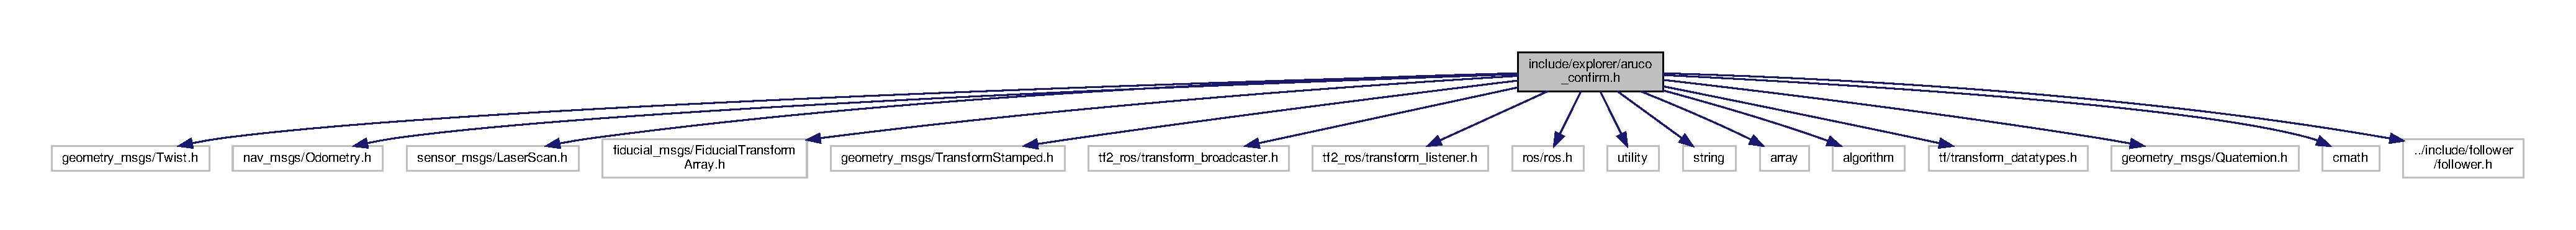
\includegraphics[width=350pt]{aruco__confirm_8h__incl}
\end{center}
\end{figure}
This graph shows which files directly or indirectly include this file\+:\nopagebreak
\begin{figure}[H]
\begin{center}
\leavevmode
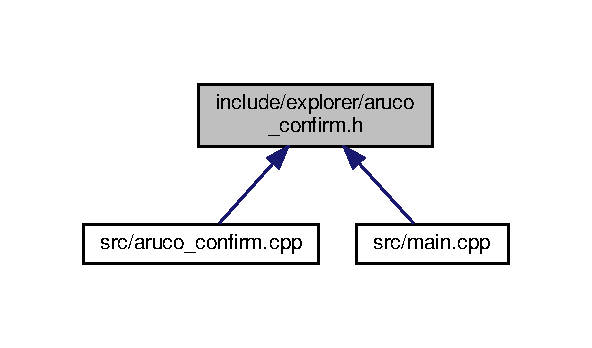
\includegraphics[width=284pt]{aruco__confirm_8h__dep__incl}
\end{center}
\end{figure}
\subsection*{Classes}
\begin{DoxyCompactItemize}
\item 
class \hyperlink{class_aruco_node}{Aruco\+Node}
\begin{DoxyCompactList}\small\item\em A class that detects the Aruco Marker. \end{DoxyCompactList}\end{DoxyCompactItemize}

\hypertarget{explorer_8h}{}\section{include/explorer/explorer.h File Reference}
\label{explorer_8h}\index{include/explorer/explorer.\+h@{include/explorer/explorer.\+h}}
{\ttfamily \#include $<$geometry\+\_\+msgs/\+Twist.\+h$>$}\newline
{\ttfamily \#include $<$geometry\+\_\+msgs/\+Quaternion.\+h$>$}\newline
{\ttfamily \#include $<$geometry\+\_\+msgs/\+Transform\+Stamped.\+h$>$}\newline
{\ttfamily \#include $<$nav\+\_\+msgs/\+Odometry.\+h$>$}\newline
{\ttfamily \#include $<$sensor\+\_\+msgs/\+Laser\+Scan.\+h$>$}\newline
{\ttfamily \#include $<$fiducial\+\_\+msgs/\+Fiducial\+Transform\+Array.\+h$>$}\newline
{\ttfamily \#include $<$move\+\_\+base\+\_\+msgs/\+Move\+Base\+Action.\+h$>$}\newline
{\ttfamily \#include $<$tf2\+\_\+ros/transform\+\_\+broadcaster.\+h$>$}\newline
{\ttfamily \#include $<$tf2\+\_\+ros/transform\+\_\+listener.\+h$>$}\newline
{\ttfamily \#include $<$tf2/\+Linear\+Math/\+Quaternion.\+h$>$}\newline
{\ttfamily \#include $<$actionlib/client/simple\+\_\+action\+\_\+client.\+h$>$}\newline
{\ttfamily \#include $<$ros/ros.\+h$>$}\newline
{\ttfamily \#include $<$utility$>$}\newline
{\ttfamily \#include $<$string$>$}\newline
{\ttfamily \#include $<$array$>$}\newline
{\ttfamily \#include $<$algorithm$>$}\newline
{\ttfamily \#include $<$iostream$>$}\newline
{\ttfamily \#include $<$tf/transform\+\_\+datatypes.\+h$>$}\newline
{\ttfamily \#include $<$cmath$>$}\newline
Include dependency graph for explorer.\+h\+:\nopagebreak
\begin{figure}[H]
\begin{center}
\leavevmode
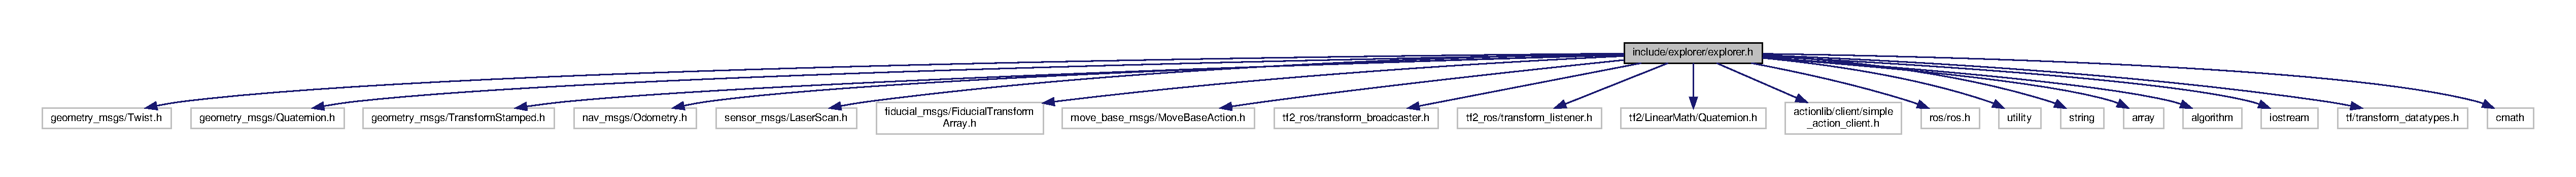
\includegraphics[width=350pt]{explorer_8h__incl}
\end{center}
\end{figure}
This graph shows which files directly or indirectly include this file\+:\nopagebreak
\begin{figure}[H]
\begin{center}
\leavevmode
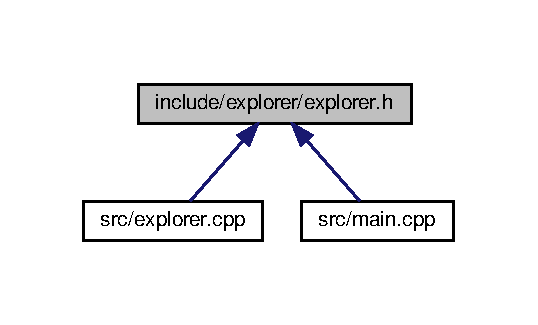
\includegraphics[width=258pt]{explorer_8h__dep__incl}
\end{center}
\end{figure}
\subsection*{Classes}
\begin{DoxyCompactItemize}
\item 
class \hyperlink{class_explorer}{Explorer}
\begin{DoxyCompactList}\small\item\em A class that inherits from Bot\+\_\+contreoller to control the explorer and exploration algorithm. \end{DoxyCompactList}\end{DoxyCompactItemize}

\hypertarget{follower_8h}{}\section{include/follower/follower.h File Reference}
\label{follower_8h}\index{include/follower/follower.\+h@{include/follower/follower.\+h}}
{\ttfamily \#include \char`\"{}../include/bot\+\_\+controller/bot\+\_\+controller.\+h\char`\"{}}\newline
Include dependency graph for follower.\+h\+:
\nopagebreak
\begin{figure}[H]
\begin{center}
\leavevmode
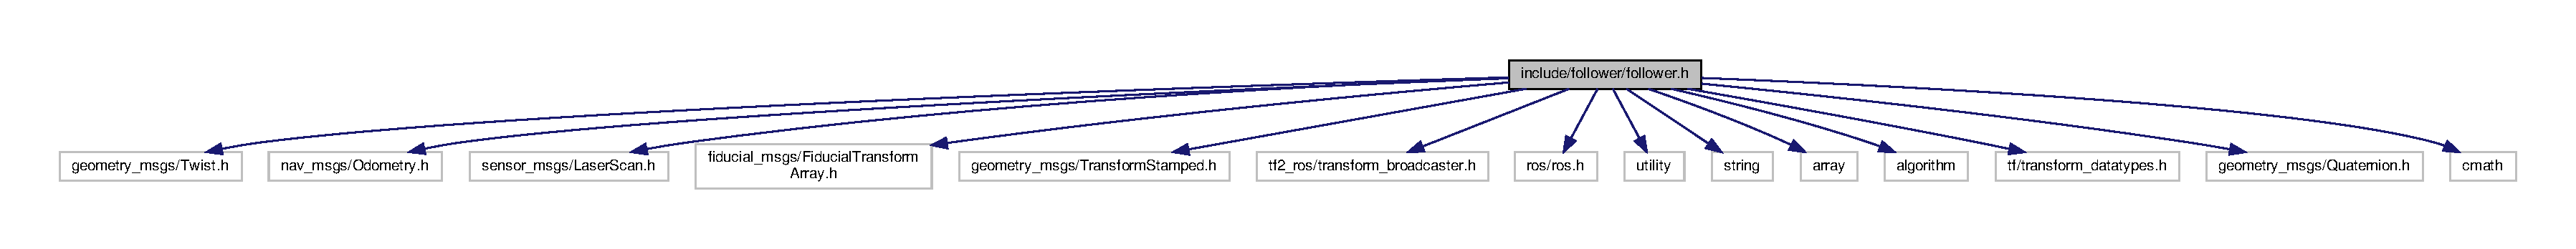
\includegraphics[width=209pt]{follower_8h__incl}
\end{center}
\end{figure}
This graph shows which files directly or indirectly include this file\+:
\nopagebreak
\begin{figure}[H]
\begin{center}
\leavevmode
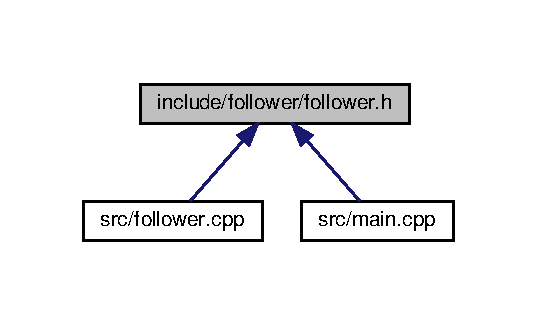
\includegraphics[width=258pt]{follower_8h__dep__incl}
\end{center}
\end{figure}
\subsection*{Classes}
\begin{DoxyCompactItemize}
\item 
class \hyperlink{class_follower}{Follower}
\begin{DoxyCompactList}\small\item\em Public Inheritance Child class of Bot\+\_\+controller Class to go to Ar\+Uco markers found by \hyperlink{class_explorer}{Explorer} child. \end{DoxyCompactList}\end{DoxyCompactItemize}

\hypertarget{_r_e_a_d_m_e_8md}{}\section{R\+E\+A\+D\+M\+E.\+md File Reference}
\label{_r_e_a_d_m_e_8md}\index{R\+E\+A\+D\+M\+E.\+md@{R\+E\+A\+D\+M\+E.\+md}}

\hypertarget{aruco__confirm_8cpp}{}\section{src/aruco\+\_\+confirm.cpp File Reference}
\label{aruco__confirm_8cpp}\index{src/aruco\+\_\+confirm.\+cpp@{src/aruco\+\_\+confirm.\+cpp}}
{\ttfamily \#include \char`\"{}../include/explorer/aruco\+\_\+confirm.\+h\char`\"{}}\newline
Include dependency graph for aruco\+\_\+confirm.\+cpp\+:\nopagebreak
\begin{figure}[H]
\begin{center}
\leavevmode
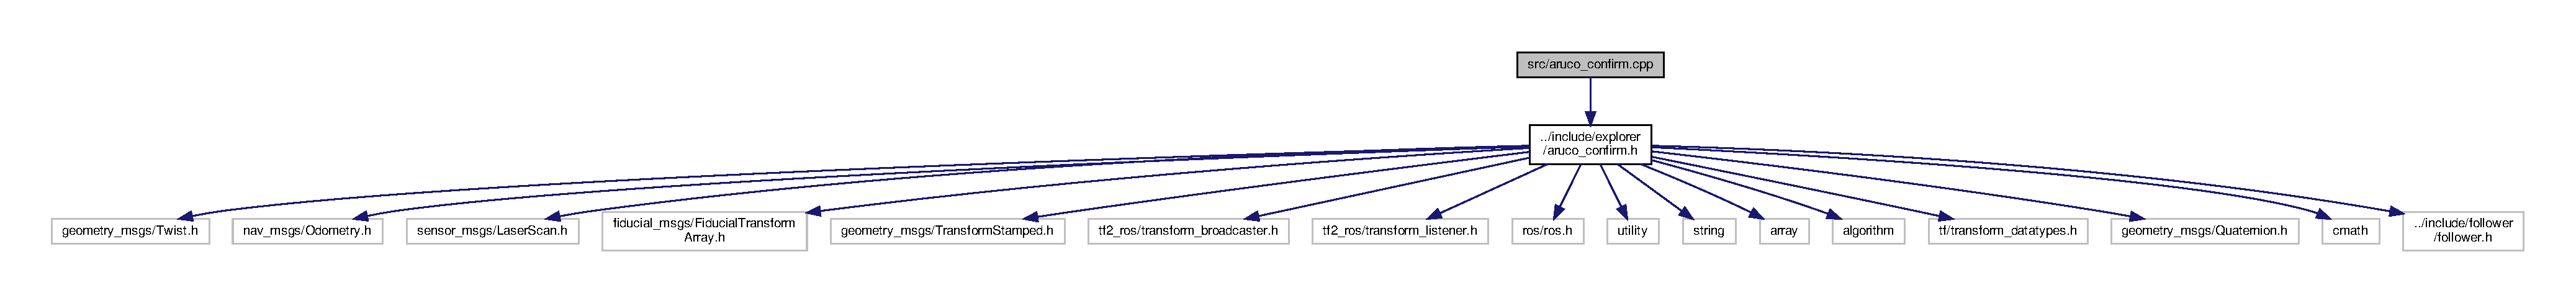
\includegraphics[width=350pt]{aruco__confirm_8cpp__incl}
\end{center}
\end{figure}

\hypertarget{explorer_8cpp}{}\section{src/explorer.cpp File Reference}
\label{explorer_8cpp}\index{src/explorer.\+cpp@{src/explorer.\+cpp}}


\hyperlink{class_aruco_node}{Aruco\+Node}.  


{\ttfamily \#include \char`\"{}../include/explorer/explorer.\+h\char`\"{}}\newline
Include dependency graph for explorer.\+cpp\+:
\nopagebreak
\begin{figure}[H]
\begin{center}
\leavevmode
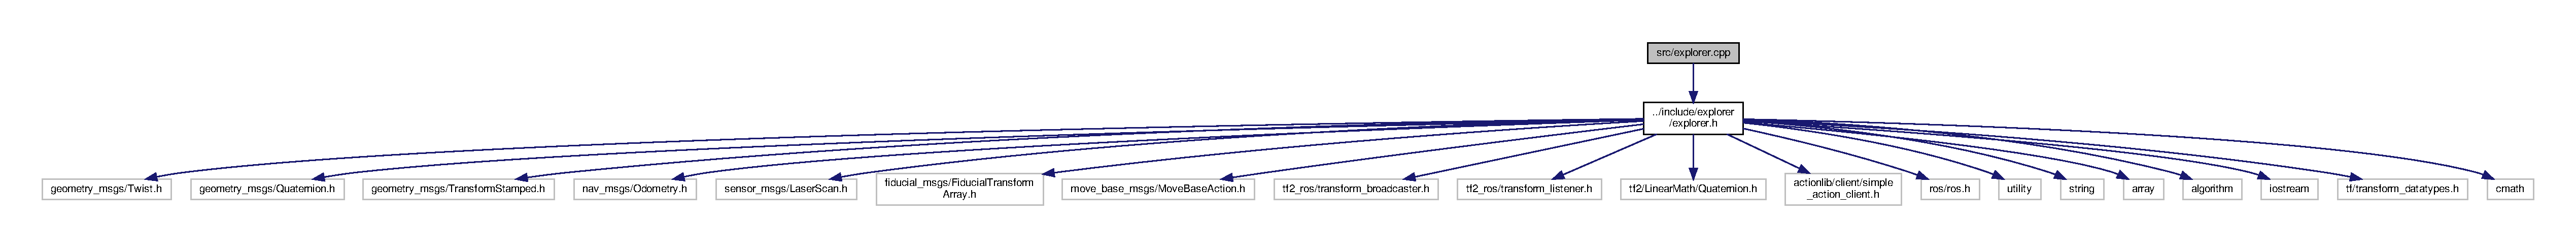
\includegraphics[width=350pt]{explorer_8cpp__incl}
\end{center}
\end{figure}
\subsection*{Functions}
\begin{DoxyCompactItemize}
\item 
std\+::array$<$ std\+::array$<$ double, 2 $>$, 4 $>$ \hyperlink{explorer_8cpp_a61450d29adf96573b7eec19cb2fa8156}{get\+\_\+goals} ()
\begin{DoxyCompactList}\small\item\em Get the goals object from aruco\+\_\+lookup.\+yaml. \end{DoxyCompactList}\end{DoxyCompactItemize}


\subsection{Detailed Description}
\hyperlink{class_aruco_node}{Aruco\+Node}. 

\hyperlink{class_explorer}{Explorer} Robot.

\begin{DoxyAuthor}{Author}
809Y Final Project Group 5 
\end{DoxyAuthor}
\begin{DoxyVersion}{Version}
0.\+1 
\end{DoxyVersion}
\begin{DoxyDate}{Date}
2021-\/12-\/12
\end{DoxyDate}
\begin{DoxyCopyright}{Copyright}
Copyright (c) 2021 
\end{DoxyCopyright}


\subsection{Function Documentation}
\mbox{\Hypertarget{explorer_8cpp_a61450d29adf96573b7eec19cb2fa8156}\label{explorer_8cpp_a61450d29adf96573b7eec19cb2fa8156}} 
\index{explorer.\+cpp@{explorer.\+cpp}!get\+\_\+goals@{get\+\_\+goals}}
\index{get\+\_\+goals@{get\+\_\+goals}!explorer.\+cpp@{explorer.\+cpp}}
\subsubsection{\texorpdfstring{get\+\_\+goals()}{get\_goals()}}
{\footnotesize\ttfamily std\+::array$<$std\+::array$<$double,2$>$,4$>$ get\+\_\+goals (\begin{DoxyParamCaption}{ }\end{DoxyParamCaption})}



Get the goals object from aruco\+\_\+lookup.\+yaml. 

\begin{DoxyReturn}{Returns}
std\+::array$<$std\+::array$<$double,2$>$,4$>$ 
\end{DoxyReturn}


Definition at line 82 of file explorer.\+cpp.


\hypertarget{follower_8cpp}{}\section{src/follower.cpp File Reference}
\label{follower_8cpp}\index{src/follower.\+cpp@{src/follower.\+cpp}}


\hyperlink{class_follower}{Follower} Robot.  


{\ttfamily \#include \char`\"{}../include/bot\+\_\+controller/bot\+\_\+controller.\+h\char`\"{}}\newline
{\ttfamily \#include \char`\"{}../include/follower/follower.\+h\char`\"{}}\newline
Include dependency graph for follower.\+cpp\+:
\nopagebreak
\begin{figure}[H]
\begin{center}
\leavevmode
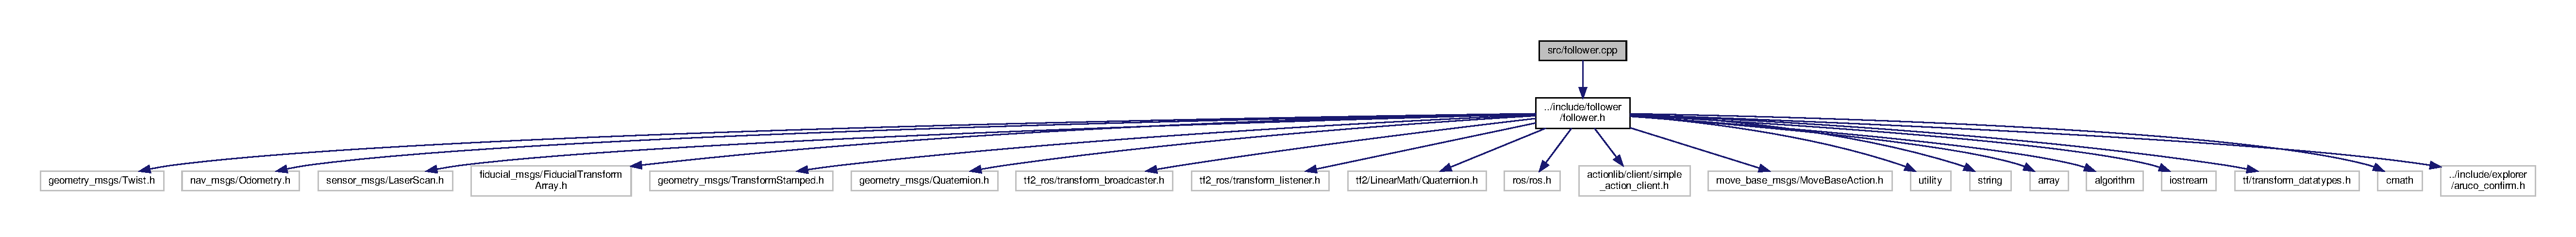
\includegraphics[width=350pt]{follower_8cpp__incl}
\end{center}
\end{figure}


\subsection{Detailed Description}
\hyperlink{class_follower}{Follower} Robot. 

\begin{DoxyAuthor}{Author}
809Y Final Project Group 5 
\end{DoxyAuthor}
\begin{DoxyVersion}{Version}
0.\+1 
\end{DoxyVersion}
\begin{DoxyDate}{Date}
2021-\/12-\/12
\end{DoxyDate}
\begin{DoxyCopyright}{Copyright}
Copyright (c) 2021 
\end{DoxyCopyright}

\hypertarget{main_8cpp}{}\section{src/main.cpp File Reference}
\label{main_8cpp}\index{src/main.\+cpp@{src/main.\+cpp}}


E\+N\+P\+M809Y Final Project Group 5.  


{\ttfamily \#include $<$actionlib/client/simple\+\_\+action\+\_\+client.\+h$>$}\newline
{\ttfamily \#include $<$fiducial\+\_\+msgs/\+Fiducial\+Transform\+Array.\+h$>$}\newline
{\ttfamily \#include $<$geometry\+\_\+msgs/\+Twist.\+h$>$}\newline
{\ttfamily \#include $<$move\+\_\+base\+\_\+msgs/\+Move\+Base\+Action.\+h$>$}\newline
{\ttfamily \#include $<$tf2/\+Linear\+Math/\+Quaternion.\+h$>$}\newline
{\ttfamily \#include $<$tf2\+\_\+ros/transform\+\_\+broadcaster.\+h$>$}\newline
{\ttfamily \#include $<$tf2\+\_\+ros/transform\+\_\+listener.\+h$>$}\newline
{\ttfamily \#include $<$ros/ros.\+h$>$}\newline
{\ttfamily \#include $<$array$>$}\newline
{\ttfamily \#include $<$iostream$>$}\newline
{\ttfamily \#include $<$algorithm$>$}\newline
{\ttfamily \#include $<$utility$>$}\newline
{\ttfamily \#include \char`\"{}../include/follower/follower.\+h\char`\"{}}\newline
{\ttfamily \#include \char`\"{}../include/explorer/explorer.\+h\char`\"{}}\newline
Include dependency graph for main.\+cpp\+:
\nopagebreak
\begin{figure}[H]
\begin{center}
\leavevmode
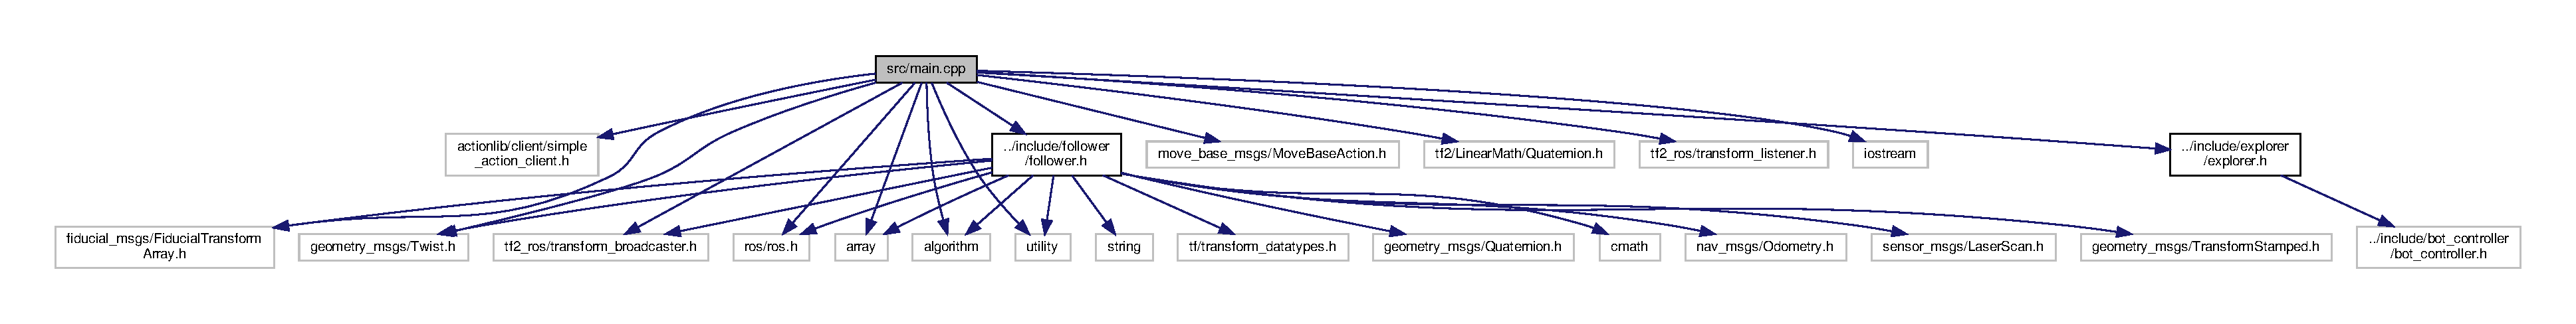
\includegraphics[width=350pt]{main_8cpp__incl}
\end{center}
\end{figure}
\subsection*{Typedefs}
\begin{DoxyCompactItemize}
\item 
typedef actionlib\+::\+Simple\+Action\+Client$<$ move\+\_\+base\+\_\+msgs\+::\+Move\+Base\+Action $>$ \hyperlink{main_8cpp_a21e20cc0b6656ae897b3cbb969b93241}{Move\+Base\+Client}
\end{DoxyCompactItemize}
\subsection*{Functions}
\begin{DoxyCompactItemize}
\item 
void \hyperlink{main_8cpp_a9c2747abcaef4c03d19858e45f59de80}{print\+\_\+usage} (std\+::string error=\char`\"{}\char`\"{})
\item 
void \hyperlink{main_8cpp_a299d89c50484c4d3a597f6b43b65e21c}{broadcast} ()
\item 
void \hyperlink{main_8cpp_aa2baabcf8bc6fb2727c0aade0c1b8efe}{listen} (tf2\+\_\+ros\+::\+Buffer \&tf\+Buffer)
\item 
int \hyperlink{main_8cpp_a3c04138a5bfe5d72780bb7e82a18e627}{main} (int argc, char $\ast$$\ast$argv)
\end{DoxyCompactItemize}


\subsection{Detailed Description}
E\+N\+P\+M809Y Final Project Group 5. 

\begin{DoxyAuthor}{Author}
Jerry Pittman, Jr., Nicholas Novak, Orlandis Smith (\href{mailto:jpittma1@umd.edu}{\tt jpittma1@umd.\+edu}, \href{mailto:nnovak@umd.edu}{\tt nnovak@umd.\+edu}, \href{mailto:osmith15@umd.edu}{\tt osmith15@umd.\+edu}) 
\end{DoxyAuthor}
\begin{DoxyVersion}{Version}
0.\+1 
\end{DoxyVersion}
\begin{DoxyDate}{Date}
2021-\/12-\/11
\end{DoxyDate}
\begin{DoxyCopyright}{Copyright}
Copyright (c) 2021 
\end{DoxyCopyright}


\subsection{Typedef Documentation}
\mbox{\Hypertarget{main_8cpp_a21e20cc0b6656ae897b3cbb969b93241}\label{main_8cpp_a21e20cc0b6656ae897b3cbb969b93241}} 
\index{main.\+cpp@{main.\+cpp}!Move\+Base\+Client@{Move\+Base\+Client}}
\index{Move\+Base\+Client@{Move\+Base\+Client}!main.\+cpp@{main.\+cpp}}
\subsubsection{\texorpdfstring{Move\+Base\+Client}{MoveBaseClient}}
{\footnotesize\ttfamily typedef actionlib\+::\+Simple\+Action\+Client$<$move\+\_\+base\+\_\+msgs\+::\+Move\+Base\+Action$>$ \hyperlink{main_8cpp_a21e20cc0b6656ae897b3cbb969b93241}{Move\+Base\+Client}}



Definition at line 29 of file main.\+cpp.



\subsection{Function Documentation}
\mbox{\Hypertarget{main_8cpp_a299d89c50484c4d3a597f6b43b65e21c}\label{main_8cpp_a299d89c50484c4d3a597f6b43b65e21c}} 
\index{main.\+cpp@{main.\+cpp}!broadcast@{broadcast}}
\index{broadcast@{broadcast}!main.\+cpp@{main.\+cpp}}
\subsubsection{\texorpdfstring{broadcast()}{broadcast()}}
{\footnotesize\ttfamily void broadcast (\begin{DoxyParamCaption}{ }\end{DoxyParamCaption})}



Definition at line 41 of file main.\+cpp.

\mbox{\Hypertarget{main_8cpp_aa2baabcf8bc6fb2727c0aade0c1b8efe}\label{main_8cpp_aa2baabcf8bc6fb2727c0aade0c1b8efe}} 
\index{main.\+cpp@{main.\+cpp}!listen@{listen}}
\index{listen@{listen}!main.\+cpp@{main.\+cpp}}
\subsubsection{\texorpdfstring{listen()}{listen()}}
{\footnotesize\ttfamily void listen (\begin{DoxyParamCaption}\item[{tf2\+\_\+ros\+::\+Buffer \&}]{tf\+Buffer }\end{DoxyParamCaption})}



Definition at line 62 of file main.\+cpp.

\mbox{\Hypertarget{main_8cpp_a3c04138a5bfe5d72780bb7e82a18e627}\label{main_8cpp_a3c04138a5bfe5d72780bb7e82a18e627}} 
\index{main.\+cpp@{main.\+cpp}!main@{main}}
\index{main@{main}!main.\+cpp@{main.\+cpp}}
\subsubsection{\texorpdfstring{main()}{main()}}
{\footnotesize\ttfamily int main (\begin{DoxyParamCaption}\item[{int}]{argc,  }\item[{char $\ast$$\ast$}]{argv }\end{DoxyParamCaption})}



Definition at line 84 of file main.\+cpp.

\mbox{\Hypertarget{main_8cpp_a9c2747abcaef4c03d19858e45f59de80}\label{main_8cpp_a9c2747abcaef4c03d19858e45f59de80}} 
\index{main.\+cpp@{main.\+cpp}!print\+\_\+usage@{print\+\_\+usage}}
\index{print\+\_\+usage@{print\+\_\+usage}!main.\+cpp@{main.\+cpp}}
\subsubsection{\texorpdfstring{print\+\_\+usage()}{print\_usage()}}
{\footnotesize\ttfamily void print\+\_\+usage (\begin{DoxyParamCaption}\item[{std\+::string}]{error = {\ttfamily \char`\"{}\char`\"{}} }\end{DoxyParamCaption})}



Definition at line 34 of file main.\+cpp.


%--- End generated contents ---

% Index
\backmatter
\newpage
\phantomsection
\clearemptydoublepage
\addcontentsline{toc}{chapter}{Index}
\printindex

\end{document}
